\documentclass[12pt]{article}
\usepackage[utf8]{inputenc}
\usepackage[spanish]{babel}

% Fuente y formato
\usepackage[T1]{fontenc} % Para las ñ y letras con tilde
% \usepackage{times}
\usepackage{microtype} % Mejora el espaciado de las palabras

% --- Fuente Helvetica en la pagina de titulo ---
\usepackage[scaled]{helvet}
\usepackage{titlesec}  % Paquete para personalizar secciones
\newcommand{\helveticatitle}{%
    \fontfamily{phv}\selectfont % Cambia a Helvetica (phv = PostScript Helvetica)
}

\usepackage{graphicx} % Required for inserting images
\usepackage{imakeidx}
\usepackage{amssymb, amsmath}
\usepackage{listings}
\usepackage{float} % Para poner las imagenes justo donde queramos

\usepackage{xcolor} % Para definir colores personalizados
\usepackage{hyperref}
\usepackage{braket}
\usepackage[braket, qm]{qcircuit}
\usepackage{subcaption}
\usepackage{url}
\usepackage{natbib}
\usepackage{bibentry}
\usepackage[nottoc]{tocbibind} % Para mostrar bibliografía no citada
\usepackage{array}
\usepackage{tikz}
\usetikzlibrary{angles, arrows.meta}


\documentclass[border=2px]{standalone}



% \setlength{\parindent}{0pt} % Elimina la sangría en todo el documento

\numberwithin{equation}{section} % Para las ecuaciones

% Definir un azul más oscuro
\definecolor{darkblue}{rgb}{0.0, 0.0, 1} % Azul oscuro

% Configuración personalizada para hyperref
\hypersetup{
    colorlinks=true,     % Colorear los enlaces en lugar de ponerles un recuadro
    linkcolor=blue,      % Color de los enlaces internos (por ejemplo, índice)
    citecolor=blue,      % Color de los enlaces de citas
    filecolor=magenta,   % Color de los enlaces a archivos
    urlcolor=blue,      % Color de los enlaces a URLs
}

\renewcommand{\UrlFont}{\sffamily\small}

\makeindex
\setlength{\parindent}{12pt}


% Márgenes de página
\usepackage[left=2.5cm, right=2.5cm, top=3cm, bottom=3cm]{geometry}

% Encabezado y pie de página guapo
\usepackage{fancyhdr}
\setlength{\headheight}{14.5pt}
\pagestyle{fancy} 
\fancyhf{} % Limpia los valores predeterminados     
\fancyhead[R]{\textit{\rightmark}} % Sección o subsección actual en la parte superior derecha
\fancyfoot[C]{\thepage} % Número de página centrado en el pie de página

% Redefinir \rightmark para mostrar jerarquía específica
\usepackage{etoolbox}
\makeatletter
\patchcmd{\sectionmark}{\markright{\thesection\ #1}}{}{}{} % Elimina la marca de sección por defecto
\renewcommand{\sectionmark}[1]{\markright{\ifnum\value{subsection}=0 \thesection\ #1 \else \ifnum\value{subsubsection}=0 \thesection\ #1 \else \rightmark \fi \fi}}
\renewcommand{\subsectionmark}[1]{\markright{\ifnum\value{subsubsection}=0 \thesubsection\ #1 \else \rightmark \fi}}
\renewcommand{\subsubsectionmark}[1]{\markright{\thesubsubsection\ #1}}
\makeatother

\usepackage{tikz}      % Paquete para gráficos y formato personalizado
% Modificar el formato de las secciones
\titleformat{\section}[block]
  {\normalfont\Huge\bfseries\raggedleft}    % Título más grande, en negrita y alineado a la derecha
  {\color{gray}\large CAPÍTULO\\}  % "Capítulo" en gris y pequeño, seguido por el número de la sección
  {\tikz[baseline]{\node[anchor=base, scale=3, text=gray, inner sep=0pt] {\thesection};} \\[1em]}  
  {\normalfont\bfseries\raggedleft}         % Título de la sección en negro, alineado a la derecha
  [\vspace{1em}]                  % Espacio después del título



\begin{document}
    \parindent=0pt

    \begin{titlepage}
        \centering
        {\fontsize{18pt}{22pt}\selectfont \textbf{\helveticatitle UNIVERSIDAD ALFONSO X EL SABIO}\par}
        \vspace{1cm}
        {\fontsize{16pt}{22pt}\selectfont \textbf{\helveticatitle ESCUELA BUSINESS \& TECH}\par}
        \vspace{1cm}
        {\fontsize{14pt}{22pt}\selectfont \textbf{\helveticatitle GRADO EN INGENIERÍA MATEMÁTICA}\par}
        \vspace{2cm}
        {
\includegraphics[width=1\textwidth]{img/portada.png}\par}
        \vspace{0.5cm}
        {\fontsize{20pt}{22pt}\selectfont \textbf{\helveticatitle TRABAJO DE FIN DE GRADO}\par}
        \vspace{1cm}
        {\fontsize{14pt}{22pt}\selectfont \textbf{\helveticatitle Computación Cuántica aplicada a la Criptografía}\par}
        \vfill
        {\fontsize{14pt}{22pt}\selectfont \textbf{\helveticatitle Rubén Nogueras González}\par}
        \vspace{1cm}
        {\fontsize{14pt}{22pt}\selectfont \textbf{\helveticatitle Junio de 2025}\par}
    \end{titlepage}


    % Segunda página con información adicional
    \newpage
    \thispagestyle{empty}
    \begin{flushleft}
        \begin{center}
            
\includegraphics[width=0.25\textwidth]{img/primera_hoja.png}\\
        \end{center}
        \begin{center}
            {\fontsize{16}{16}\selectfont \textbf{\helveticatitle UNIVERSIDAD ALFONSO X EL SABIO}}\\
            {\fontsize{14}{14}\selectfont \textbf{\helveticatitle ESCUELA BUSINESS \& TECH}}\\[0cm]
            {\fontsize{12}{12}\selectfont \textbf{\helveticatitle GRADO EN INGENIERÍA MATEMÁTICA}}\\[0cm]
            \textbf{}\\[0.3cm]
            {\fontsize{14}{14}\selectfont \textbf{\helveticatitle COMPUTACIÓN CUÁNTICA APLICADA A LA CRIPTOGRAFÍA}}\\[0cm]
        \end{center}

        {\fontsize{12}{12}\selectfont \textbf{\helveticatitle ALUMNO:}} \helveticatitle RUBÉN NOGUERAS GONZÁLEZ\\
        {\fontsize{12}{12}\selectfont \textbf{\helveticatitle N.P.:}} \helveticatitle 139174\\
        {\fontsize{12}{12}\selectfont \textbf{\helveticatitle TUTOR ACADÉMICO:}} \helveticatitle JOSÉ ANTONIO PRIETO PERSIGUERO\\
        {\fontsize{12}{12}\selectfont \textbf{\helveticatitle FECHA DE PRESENTACIÓN:} 13/06/2025}\\
        {\fontsize{12}{12}\selectfont \textbf{\helveticatitle BREVE DESCRIPCIÓN:}}
    \end{flushleft}

    {\fontsize{12}{12}\selectfont \helveticatitle
    
    }

    {\fontsize{10}{10}\selectfont
    \noindent  \textbf{\helveticatitle FIRMA DEL DIRECTOR DEL TRABAJO:}\hspace{4cm}\textbf{\helveticatitle FIRMA DEL ALUMNO:}}
    
    % Pagina en blanco
    \newpage
    \thispagestyle{empty}
    \mbox{}
    \newpage

    \tableofcontents

    % Pagina en blanco
    \newpage
    \thispagestyle{empty}
    \mbox{}

    \listoffigures

    % Pagina en blanco
    \newpage
    \thispagestyle{empty}
    \mbox{}
    \newpage


    \thispagestyle{empty}
    \section{Introducción}
        \subsection{Objetivos}

        \vspace{5mm}

        \begin{itemize}
            \item Comprender la necesidad de la mecánica cuántica en la física clásica.
            \item Entender los fundamentos matemáticos de la mecánica cuántica, incluyendo álgebra lineal y espacios de Hilbert.
            \item Aprender las diferencias, ventajas y desventajas entre un ordenador cuántico y uno tradicional.
            \item Analizar el papel que juegan las puertas cuánticas en la manipulación de estados, y por lo tanto en algoritmos cuánticos.
            \item Explicar los distintos principios básicos de la criptografía cuántica para garantizar la seguridad de los nuevos sistemas.
            \item Aprender el concepto de teleportación cuántica como mecanismo eficiente y seguro para la transmisión de información.
        \end{itemize}

        \vspace{5mm}

        \subsection{Historia de la Mecánica Cuántica}\label{sec: historia}

        \vspace{5mm}

        La computación cuántica es un nuevo sistema de computación, en el que nos apoyamos en las propiedades de los sistemas cuánticos para mejorar distintos paradigmas de la computación clásica. Esto lo hacemos mediante el uso del \textit{qubit}, la unidad básica de información cuántica, a diferencia de la información clásica que se centra en el \textit{bit} como unidad minima de información. La principal ventaja de los \textit{qubits} es que, además de albergar información binaria (0 o 1), podemos obtener una mezcla de ambos estados (esto se conoce como el principio de superposición cuántica, que ya veremos en los próximos capítulos), de manera que podemos obtener algoritmos cuánticos que no pueden ser modelizados mediante \textit{bits}, reduciendo en muchos casos la complejidad de algoritmos clásicos tradicionales, lo que mejora el rendimiento y eficiencia de nuestros computadores.

        \vspace{5mm}

        Para explicar esto de la mejor manera posible, nos remontamos a los orígenes de la física cuántica, a finales del siglo \textit{XIX} y principios del siglo \textit{XX}, cuando se pensaba que la física clásica era el foco global para explicar todos los fenómenos que suceden a nuestro alrededor, hasta que con el resultado de ciertos experimentos se comenzó a ver una relación entre el comportamiento de las ondas y las partículas, rompiendo completamente con los principios de la física clásica.

        \vspace{5mm}

        En primer lugar, vamos a comenzar explicando qué es un cuerpo negro, esto es un cuerpo que absorbe toda la radiación emitida sobre él, sin reflejar nada de lo que le llega. Esto se puede imaginar como una cavidad isotérmica con un orificio por el que se aproxima cierta radiación, de manera que permanezca en su interior. Además, suponemos que dicha cavidad se encuentra en equilibrio térmico, es decir, a una temperatura constante, de manera que la radiación que permanece dentro de ella se transforma en energía, obligando a emitir radiación hacia el exterior, sin tener nada que ver con la radiación que entra por el orificio.

        \vspace{5mm}

        \begin{figure}[H]
            \centering
            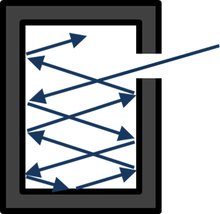
\includegraphics[width=0.2\textwidth]{img/Introduccion/cavidad_cuerpo_negro2.png}
            \caption{Ilustración del cuerpo negro. Obtenida de~\cite{fisica2022}}.\label{fig: f1}
        \end{figure}
        
        \vspace{5mm}

        La física clásica es incapaz de explicar la radiación emitida por un cuerpo negro en función de la longitud de onda,
        hasta que la explicación de este fenómeno vino de la mano de \textit{Max Planck} en el siglo \textit{XX}, el cual establece que la energía liberada por el cuerpo negro se emite en pequeños paquetes, llamados \textit{cuantos de energía}. Esta energía es proporcional a una pequeña constante, la constante de Planck, de manera que la energía emitida por el cuerpo negro no es continua, sino que toma un valor discreto que ha de ser múltiplo de dicha constante por su frecuencia de onda, rompiendo completamente con la física de la época y dando el nacimiento a un nuevo campo de la física, la mecánica cuántica.

        \vspace{5mm}

        \begin{equation}
            E = h \nu
            \label{eq: planck}
        \end{equation}

        \vspace{5mm}

        Siendo \( h \) la denominada \textit{constante de Planck}, la cual alcanza un valor de \( 6.62607015 \times 10^{-34} \, \text{J} \cdot \text{s} \), y siendo \( \nu \) la frecuencia. Esta energía o intensidad que libera el cuerpo la podemos medir, en función de su longitud de onda, obteniendo la siguiente gráfica:

        \vspace{5mm}

        \begin{figure}[H]
            \centering
            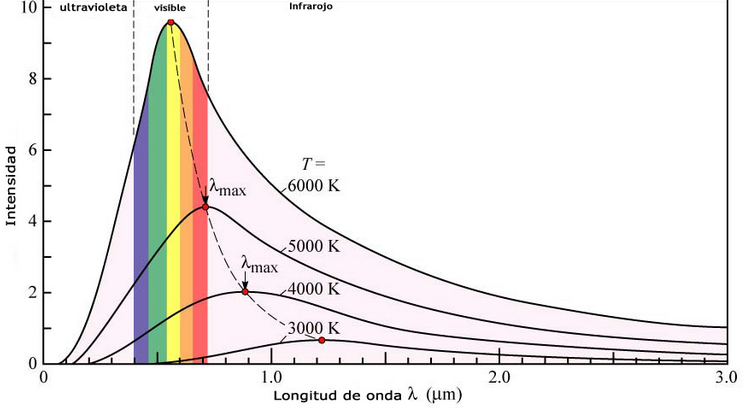
\includegraphics[width=0.75\textwidth]{img/Introduccion/catastrofe_ultravioleta.png}
            \caption{Catástrofe del ultravioleta. Obtenida de~\cite{weblab2013}}
            \label{fig: f2}
        \end{figure}

        \vspace{5mm}

        Podemos observar que a diferentes temperaturas (longitudes de onda) llegamos a diferentes curvas. La física clásica intentaba predecir estas curvas mediante ciertos modelos, que, aunque se ajustaban correctamente en distintas zonas de la gráfica, no se acercaban ni mucho menos a la realidad. Un ejemplo de esto es la catástrofe del ultravioleta, como resultado de no ajustarse correctamente en la zona ultravioleta, en la que la intensidad de la energía tendía a infinito como resultado de otros modelos, en lugar de tender a cero como propuso \textit{Max Planck}, formulando una ecuación que describe perfectamente la figura (\ref{fig: f2}):

        \vspace{5mm}

        \begin{equation}
            B_{\nu}(T) = \frac{2h\nu^3}{c^2} \frac{1}{e^{\frac{h\nu}{k_B T}} - 1}
            \label{eq: planck_ultravioleta}
        \end{equation}

        \vspace{5mm}

        Donde \textit{h} es la \textit{constante de Planck}, \( \nu \) la frecuencia de la radiación, \textit{c} la velocidad de la luz en el vacío, \( k_B \) la \textit{constante de Boltzmann}, \textit{T} la temperatura, y \textit{e} como base de los logaritmos naturales. No obstante, esta teoría cuántica fue primeramente descartada por los físicos de la época, al establecer que la energía no es un valor continuo sino discreto, hasta que con la llegada del efecto fotoeléctrico de \textit{Albert Einstein} todo comenzó a cobrar sentido.

        \vspace{5mm}    

        A finales del siglo XIX, en 1888, se presenta el efecto fotoeléctrico, definido por \textit{Heinrich Hertz}, que consiste en la emision de electrones (fotoelectrones) al incidir luz sobre un metal, actuando como cátodo, los cuales se recogen en un ánodo, generando corriente en un circuito. Dicha luz suele ser ultravioleta, aunque en algunos casos puede ser visible.

        \vspace{5mm}

        Previamente al experimento, se plantearon varias hipótesis en base a la física clásica de la época:

        \begin{itemize}
            \item El aumento de la intensidad de la luz incrementaría la energía cinética de los fotoelectrones emitidos.
            \item A mayor frecuencia mayor intensidad de corriente en el circuito. 
        \end{itemize}

        \vspace{5mm}

        Los resultados de dicho experimento fueron sorprendentes, ya que se observó que la energía cinetica de los electrones que poseen el cátodo no dependen de la intensidad de la luz, sino de su frecuencia, y adicionalmente se pudo ver que a mayor intensidad de luz mayor intensidad de corriente. Más tarde, en 1905, se presentó un artículo, ciertamente atrevido teniendo en cuenta los recursos de la época, que resolvía todos estos problemas.

        \vspace{5mm}

        \textit{Albert Einstein} presentó su hipótesis para el efecto fotoeléctrico, basándose en los resultados del experimento de \textit{Planck}, aclarando que la luz no se comporta como una onda, sino que está compuesta de pequeñas partículas, llamadas \textit{fotones}, cuya energía depende de su frecuencia, como ya propuso \textit{Max Planck} en (\ref{eq: planck}), rompiendo de nuevo con los principios de la física clásica.

        \vspace{5mm}

        En dicha hipótesis se establece la necesidad de una frecuencia mínima, denominada frecuencia umbral, para que el efecto fotoeléctrico tenga lugar, la cual depende del material del que esté construido el cátodo. Por lo que si la frecuencia de los \textit{fotones} emitidos por el haz de luz es menor a esta frecuencia umbral, no se produce corriente en el circuito, por muy intensa que sea la luz. De esta manera, si la frecuencia es mayor o igual a la umbral, los \textit{fotoelectrones} se trasladarán hacia el ánodo al ser expulsados del núcleo de sus átomos, generando energía cinética y por lo tanto, intensidad de corriente en el circuito. Esto lo podemos razonar con la siguiente ecuación:

        \vspace{5mm}

        \begin{equation}
            E_e = E_{ionizacion} + E_{cinetica}
            \label{eq: einstein_fotoelectrico}
        \end{equation}

        \vspace{5mm}

        Esta ecuación tiene sentido visto lo anterior, de manera que la energía de los electrones del cátodo ha de ser igual a su \textit{energía de ionización} (o también conocido como \textit{trabajo de extracción}), la cual es la cantidad de energía necesaria para que se produzca el efecto fotoeléctrico, sumado a su \textit{energía cinética}. Por la explicación vista anteriormente, sabemos que dicha \textit{energía de ionización} depende de la \textit{frecuencia umbral \( \nu_{0} \)}, y con la ecuación de la energía de \textit{Planck} (\ref{eq: planck}), además de conocer la \textit{energía cinética} de una partícula, podemos desarrollar la expresión (\ref{eq: einstein_fotoelectrico}):

        \vspace{5mm}

        \begin{equation*}
            h \nu = h \nu_{0} + \frac{1}{2} m_{e} v_{e}^{2}
        \end{equation*}

        \vspace{5mm}

        Donde \textit{h} es la \textit{constante de Planck}, \( \nu \) es la \textit{frecuencia}, \( \nu_{0} \) es la \textit{frecuencia umbral}, \( m_{e} \) es la masa del electrón, y \( v_{e} \) la velocidad del electrón, en este caso al cuadrado. 
        
        \vspace{5mm}

        Estos son solo dos de los múltiples experimentos con soluciones extrañas para los físicos clásicos de aquella época, en los que, como hemos visto, el comportamiento de ciertos fenómenos, teóricamente imaginados como funciones de onda, se comportan como partículas. También se da el fenómeno contrario, experimentos planteados como partículas pero que son razonados mediante funciones de onda. Esto se definió con el nombre de \textit{dualidad onda-corpúsculo}.
        
        \vspace{5mm}

        Más tarde, tras estudiar a fondo las bases de la mecánica cuántica propuesta por \textit{Max Planck} y \textit{Albert Einstein}, \textit{Louis de Broglie} propuso en su tesis doctoral, en \textit{1924}, que no solo la luz tiene un carácter ondulatorio, sino que toda partícula material, como los electrones, tienen una naturaleza ondulatoria, cuya longitud de onda \( \lambda \) es:
        
        \vspace{5mm}

        \begin{equation}
            \lambda = \frac{h}{p}
            \label{eq: longitud de onda}
        \end{equation}

        \vspace{5mm}

        Donde \textit{p} se refiere al \textit{momento lineal} de la partícula, lo cual podemos expresar como \( p = m \cdot v \), siendo \textit{m} la masa, y \textit{v} la velocidad de la partícula. Tras el razonamiento de \textit{Broglie} en \textit{1924}, surge la \textit{función de onda} en una dimensión, la cual describe el comportamiento las partículas con carácter ondulatorio:

        \vspace{5mm}

        \begin{equation}
            \varphi (x, t) = e^{i(px - Et) / \hbar}
            \label{eq: funcion_de_onda}
        \end{equation}

        \vspace{5mm}

        Siendo \textit{i} la unidad imaginaria, \( \hbar \) la \textit{constante de Planck normalizada}

        \vspace{5mm}

        \begin{equation}
            \hbar = \frac{h}{2\pi} 
            \label{constante_planck_normalizada}
        \end{equation}    

        \vspace{5mm}
        
        y \textit{x} y \textit{t} las coordenadas de posición y tiempo de la partícula. Sin embargo, todavia no se conocia su significado fisico con total exactitud. No fue hasta que con el experimento de la doble rendija de \textit{Clinton Davisson} y \textit{Lester Germer} sobre electrones en \textit{1927} (aunque \textit{Thomas Young} lo propuso en \textit{1801}, sobre un haz de luz, demostrando su naturaleza ondulatoria) que se confirmó la hipótesis de \textit{De Broglie}. Como su propio nombre indica, dicho experimento consiste en una superficie opaca con dos rendijas, detrás de la cual colocamos un detector de partículas para poder percibir el comportamiento de los electrones o fotones que pasan a través de ambas rendijas. Según la física clásica, se espera que las partículas pasen a través de las rendijas en forma de línea recta, como lo haría cualquier objeto. Sin embargo, esto no sucede así en el contexto de la mecánica cuántica.

        \vspace{5mm}

        \begin{figure}[H]
            \centering
            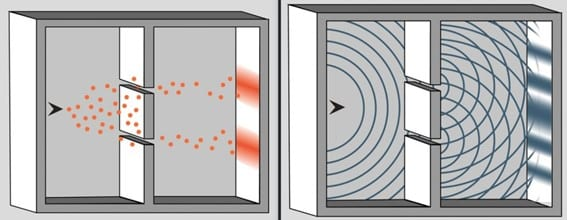
\includegraphics[width=0.75\textwidth]{img/Introduccion/doble_rendija.png}
            \caption{Experimento de la doble rendija. Obtenida de~\cite{dciencia2021}}\label{fig: doble_rendija}
        \end{figure}

        \vspace{5mm}

        Al realizar el experimento, podemos observar un patrón de interferencias en la pantalla de detección situada detrás de las rendijas, el cual es muy similar al patrón que siguen las ondas cuando se superponen unas con otras. Efectivamente, las ondas asociadas a cada partícula se superponen unas con otras como se reveló en el experimento, no obstante, cuando observamos estas partículas mediante el detector, se comportan como una partícula clásica, cambiando su comportamiento, de manera que podemos ver por qué rendija cruzó la partícula. Este fenómeno se conoce como \textit{colapso de función de onda}, y existen muchas teorías que intentar explicar esto, siendo la más famosa la \textit{intepretación de Copenhage}, en la que se establece que la observación de la partícula produce un colapso de su función de onda, determinando su estado correspondiente a la medición.

        \vspace{5mm}

        Matemáticamente, podemos expresar la superposición de ondas como una superposición de estados, esto es:

        \vspace{5mm}

        \begin{equation}
            \psi(x, t) = \psi_{1}(x, t) + \psi_{2}(x, t) + \dots + \psi_{n}(x, t), \qquad \forall n \in \mathbb{N} \setminus \{0\}
            \label{eq: superposicion}
        \end{equation}

        \vspace{5mm}

        Adicionalmente, surgieron ciertas dudas relacionadas con la naturaleza de la función de onda. Es lógico preguntarse que, si las partículas están definidas por funciones de onda, ¿Dónde están realmente las partículas? Ya que una partícula no puede estar en varios puntos a la vez, ha de estar en un único punto. Es aquí cuando entró \textit{Max Born}, quien sugiere que \( \lvert \psi(x, t) \rvert ^ {2} \) no es simplemente el cuadrado del módulo de la función de onda, sino que es una función de densidad de probabilidad, de manera que, para cada instante de tiempo y una región del espacio, la siguiente integral

        \vspace{5mm}

        \begin{equation}
            \int_{E} \lvert \psi(x, t) \rvert ^ {2} dx, \qquad \forall t \in \mathbb{R}, E \subset \Omega
            \label{eq: densidad_probabilidad_onda}
        \end{equation}

        \vspace{5mm}

        Representa la densidad de probabilidad de encontrar una partícula para un valor de \textit{t} en una determinada región \textit{E} del espacio \( \Omega \), de manera que podemos deducir una condición que ha de cumplir la expresión (\ref{eq: densidad_probabilidad_onda}):
        
        \vspace{5mm}

        \begin{equation}
            \int_{\Omega} \lvert \psi(x, t) \rvert ^ {2} dx = 1, \qquad \forall t \in \mathbb{R}
            \label{eq: interpretacion_probabilistica}
        \end{equation}

        \vspace{5mm}
        
        Esto tuvo una importancia bastante profunda en la mecánica cuántica de la época y en la física en general, ya que las únicas ideas de probabilidad estaban relacionadas a sistemas de incertidumbre, como el lanzamiento de una moneda. De esta manera se concluyó en la probabilidad como uno de los principales focos de la física y de la comprensión de las partículas subatómicas.

        \vspace{5mm}

        Esto concluye, al no poder medir con exactitud el estado de una partícula, como ocurre en la física clásica, en el \textit{principio de incertidumbre} de \textit{Heisenberg} en \textit{1927}, estableciéndose que en la medición de una partícula no podemos conocer con completa exactitud la posición y el momento lineal a la vez, sino que cuanto más preciso midamos su posición exacta menos precisa será la medición del momento lineal de dicha partícula y viceversa.

    \vspace{5mm}





    \newpage
    \thispagestyle{empty}
    \mbox{}

    \section{La Ecuación de Schrödinguer}\label{sec: la_ecuacion_de_schrodinguer}

    \subsection{Obtención de la Ecuación de Schrödinguer}

    \vspace{5mm}

    Todas las ideas vistas anteriormente, la función de onda (\ref{eq: funcion_de_onda}), la superposición cuántica (\ref{eq: superposicion}) y la interpretacion probabilística de la función de onda (\ref{eq: densidad_probabilidad_onda}) dieron lugar a la necesidad de decribir la evolución de la función de onda \( \psi(x, t) \) en función del tiempo \textit{t}. Es en este momento cuando aparece \textit{Erwin Schrödinguer} en \textit{1926}, presentando su famosa ecuación, obtenida de derivar y desarrollar la ecuación  (\ref{eq: funcion_de_onda}). En primer lugar, derivamos dicha expresión (\ref{eq: funcion_de_onda}) con respecto al tiempo \textit{t}:

    \begin{align*}
        \frac{\partial}{\partial t} \psi(x, t) &= \frac{\partial}{\partial t} e^{i(px - Et) / \hbar} \\[8pt]
        \frac{\partial}{\partial t} \psi(x, t) &= e^{i(px - Et) / \hbar} \left(- \frac{iE}{\hbar} \right)
    \end{align*}

    \vspace{2.5mm}

    Podemos observar que vuelve a aparecer la función de onda (\ref{eq: funcion_de_onda}), al tratarse de una función exponencial:

    \begin{equation*}
        \frac{\partial}{\partial t} \psi(x, t) = - \frac{iE}{\hbar} \psi(x, t)
    \end{equation*}

    \vspace{2.5mm}

    A continuación multiplicamos ambos miembros por \( i\hbar \), para eliminar los denominadores y substrayendos de la expresión:

    \begin{equation}
        i \hbar \frac{\partial}{\partial t} \psi(x, t) = E \psi(x, t)
        \label{eq: obtencion_schrodinguer}
    \end{equation}

    \vspace{2.5mm}

    Esta expresión la reservaremos para más adelante, ya que, en los siguientes cálculos, necesitaremos el producto de la energía del sistema \( E \) y la función de onda \( \psi \). Como siguiente paso, vamos a continuar derivando la función de onda (\ref{eq: funcion_de_onda}) con respecto de \textit{x}:

    \begin{align*}
        \frac{\partial}{\partial x} \psi(x, t) &= \frac{\partial}{\partial x} e^{i(px - Et) / \hbar} \\[10pt]
        \frac{\partial}{\partial x} \psi(x, t) &= e^{i(px - Et) / \hbar} \left( \frac{ip}{\hbar} \right) \\[10pt]
        \frac{\partial}{\partial x} \psi(x, t) &= \frac{ip}{\hbar} \psi(x, t)
    \end{align*}

    \vspace{2.5mm}

    Derivamos por segunda vez respecto de la variable espacial:

    \begin{align*}
        \frac{\partial}{\partial x^{2}} \psi(x, t) &= \frac{\partial}{\partial x} \left( \frac{ip}{\hbar} \psi(x, t) \right) \\[10pt]
        \frac{\partial}{\partial x^{2}} \psi(x, t) &= - \frac{p^{2}}{\hbar^{2}} \psi(x, t)
    \end{align*}

    \vspace{2.5mm}

    Multiplicamos por (\( - \frac{\hbar^{2}}{2m} \)) para obtener lo siguiente:

    \begin{equation*}
        - \frac{\hbar^{2}}{2m} \frac{\partial}{\partial x^{2}} \psi(x, t) = \frac{p^{2}}{2m} \psi(x, t)
        \\[2mm]
    \end{equation*}

    \vspace{2.5mm}

    Conociéndose que la energía cinética es \( E = \frac{p^{2}}{2m} \), obtenemos la siguiente expresión

    \begin{equation*}
        - \frac{\hbar^{2}}{2m} \frac{\partial}{\partial x^{2}} \psi(x, t) = E \psi(x, t)
    \end{equation*}

    \vspace{2.5mm}

    Sustituyendo el valor que acabamos de obtener \( E \psi(x, t) \) en (\ref{eq: obtencion_schrodinguer}), llegamos prácticamente a la ecuación que estamos buscando:

    \begin{equation*}
        i \hbar \frac{\partial}{\partial t} \psi(x, t) = - \frac{\hbar^{2}}{2m} \frac{\partial}{\partial x^{2}} \psi(x, t)
        \\[2mm]
    \end{equation*}

    \vspace{2.5mm}

    Para terminar, si agregamos la energía potencial y generalizamos la ecuación para más de una dimensión espacial, obtenemos la famosa \textbf{\textit{ecuación de Schrödinguer}}:

    \begin{equation}
        \boxed{i \hbar \frac{\partial}{\partial t} \psi(x, t) = (- \frac{\hbar^{2}}{2m} \Delta + V(x, t)) \psi(x, t)} 
        \label{eq: ecuacion_schrodinguer}     
    \end{equation}

    \vspace{2.5mm}

    Siendo \( \Delta \) el operador Laplaciano en coordenadas canónicas, que se define como

    \begin{equation*}
        \Delta = \frac{\partial}{\partial^{2} x_{1}} + \cdots + \frac{\partial}{\partial^{2} x_{n}}, \qquad \forall n \in \mathbb{N}
    \end{equation*}

    \vspace{5mm}





    \subsection{La Ecuación de Schrödinguer Independiente del Tiempo}

    \vspace{5mm}

    A continuación, para obtener la \textit{ecuación de Schrödinguer independiente del tiempo} tenemos que plantearnos obtener las soluciones de la ecuación de Schrödinguer (\ref{eq: ecuacion_schrodinguer}). Para simplificar cálculos, vamos a suponer que la energía potencial \( V(x) \) en (\ref{eq: ecuacion_schrodinguer}) depende única y exclusivamente de la variable espacial \textit{x}, de manera que podemos probar a encontrar soluciones por el método de \textit{separación de variables}. Supongamos una solución como producto de dos funciones \( \psi(x) \) y \( \tau(t) \):

    \begin{equation*}
        \Psi(x, t) = \psi(x) \tau(t) \\[5pt]
    \end{equation*}

    \vspace{2.5mm}

    Sustituyendo en (\ref{eq: ecuacion_schrodinguer}) nos queda como

    \begin{equation*}
        i \hbar \frac{\partial}{\partial t} \psi(x) \tau(t) = \left( - \frac{\hbar^{2}}{2m} \Delta + V(x) \right) \psi(x) \tau(t) \\[5pt]
    \end{equation*}

    \vspace{2.5mm}

    Podemos dividir entre \( \psi(x) \tau(t) \) y ordenar ambos miembros, de manera que un miembro nos quede únicamente en función de \textit{x} y otro en función de \textit{t}:

    \begin{equation*}
        i \hbar \frac{1}{\tau(t)} \frac{\partial}{\partial t} \tau(t) = V(x) - \frac{\hbar^{2}}{2m} \frac{1}{\psi(x)} \frac{\partial}{\partial x^{2}} \psi(x) \\[5pt]
    \end{equation*}

    \vspace{2.5mm}

    Hemos de recalcar que hemos tomado el laplaciano \( \Delta \) como \( \frac{\partial}{\partial x^{2}} \), siendo este el laplaciano en una dimensión espacial, con el fin de simplificar los cálculos. Llegados a este punto, para que se cumpla la igualdad, cada miembro de la ecuación ha de ser igual a una constante \( E \), al demostrarse que se trata de una ecuación separable
    
    \begin{equation}
        \begin{cases}
            \displaystyle i \hbar \frac{1}{\tau(t)} \frac{\partial}{\partial t} \tau(t) = E \\[10pt]
            \displaystyle V(x) - \frac{\hbar^{2}}{2m} \frac{1}{\psi(x)} \frac{\partial}{\partial x^{2}} \psi(x) = E \\[10pt]
        \end{cases}
        \label{eq: separacion_variables}
    \end{equation}

    \vspace{2.5mm}

    Tomando como base la primera ecuación del sistema, podemos obtener una solución exponencial de la siguiente manera:
        
    \begin{align*}
        \frac{\partial}{\partial t} \tau(t) &= \frac{E}{i \hbar} \tau(t) \\[10pt]
        \tau(t) &= e ^ { \left( - \frac{Ei}{\hbar} \right) t}
    \end{align*}

    \vspace{2.5mm}

    Esto nos proporciona una evolución temporal del sistema en el que se encuentra la partícula. Sin embargo, para obtener la ecuación que estamos buscando, hemos de fijarnos en la segunda ecuación de (\ref{eq: separacion_variables}):

    \begin{equation*}
        V(x) - \frac{\hbar^{2}}{2m} \frac{1}{\psi(x)} \frac{\partial}{\partial x^{2}} \psi(x) = E
    \end{equation*}

    \vspace{2.5mm}

    La cual podemos reescribir como

    \begin{equation}
        \left( - \frac{\hbar^{2}}{2m} \frac{\partial}{\partial x^{2}} + V(x) \right) \psi(x) = E \psi(x) \\[5pt]
        \label{eq: schrodinguer_independiente_tiempo}
    \end{equation}

    \vspace{2.5mm}

    En muchas referencias, la ecuación (\ref{eq: schrodinguer_independiente_tiempo}) es ya la ecuación que estamos buscando. Sin embargo, nosotros la vamos a denotar en función del operador \textit{Hamiltoniano} \( H \), el cual representa la energía total de nuestro sistema cuando ésta permanece constante en el tiempo, que en nuestro caso sucede al establecer que \( V(x, t) = V(x) \). Así, la \textbf{\textit{ecuación de Schrödinguer independiente del tiempo}} queda como
    
    \begin{equation}
        \boxed{ H \psi(x) = E \psi(x)}
        \label{eq: schrodinguer_independiente_tiempo_hamiltoniano}
    \end{equation}

    \vspace{2.5mm}

    Siendo \( H = \left( - \frac{\hbar^{2}}{2m} \frac{\partial}{\partial x^{2}} + V(x) \right) \) el operador \textit{Hamiltoniano}. Finalmente, podemos concluir que la solución completa queda como

    \begin{equation}
        \Psi(x, t) = e ^ { \left( - \frac{Ei}{\hbar} \right) t} \psi(x)
    \end{equation}

    \vspace{5mm}

    La ecuación (\ref{eq: schrodinguer_independiente_tiempo_hamiltoniano}) describe los estados estacionarios de una partícula en el potencial \( V(x) \) y es usada en muchos sistemas físicos de vital importancia (generalmente aquellos cuyo potencial no depende del tiempo \( t \)) como átomos y moléculas en estado estacionario, siempre y cuando el sistema se encuentre en equilibrio y no haya fuerzas externas que varíen el valor de la energía potencial con respecto al tiempo, pozos de potencial infinito, osciladores armónicos, o campos eléctricos y gravitacionales constantes.

    \vspace{5mm}

    Sin embargo, hay otras muchas situaciones en las que el potencial no solo depende de la posición \( x \), de manera que no podemos aplicar el método de separación de variables visto anteriormente, como partículas en campos magnéticos, problemas asociados a la relatividad, o sistemas caóticos. Para estos sistemas utilizamos otros métodos de resolución, como simulaciones numéricas, para alcanzar la solución del sistema.

    \vspace{5mm}


    


    \newpage
    \thispagestyle{empty}
    \mbox{}

    \section{El Espacio de Hilbert}\label{sec: el_espacio_de_Hilbert}

    \vspace{5mm}

    En el contexto de la mecánica cuántica, el \textit{espacio de Hilbert}, el cual denotaremos como \( \mathcal{H} \), es el marco matemático en el que nos apoyamos para explicar el estado físico de las partículas subatómicas, como ya veremos en la sección (\ref{sec: postulados}) explicando los postulados. Este \textit{espacio de Hilbert} es simplemente una generalización de los espacios euclídeos \( \mathbb{R}^{n} \) sobre el cuerpo de los números reales \( \mathbbl{R} \) o sobre los números complejos \( \mathbb{C} \), siendo en el caso de la mecánica cuántica, como podremos imaginar, una generalización sobre \( \mathbb{C} \) ya que la geometría compleja juega un papel fundamental en este campo de la física.
    
    \vspace{5mm}

    Una vez hemos introducido los \textit{espacios de Hilbert}, vamos a pasar a explicar sus propiedades básicas, para poder comprender los conceptos que vendrán más adelante en los siguientes capítulos. La diferencia fundamental con respecto a los espacios euclídeos \( \mathbb{R}^{n} \), además de que las distintas componentes de los vectores \( \ket{\psi} \in \mathcal{H} \) son complejas, reside en el producto escalar, el cual para un espacio euclídeo \( \mathbb{R}^{n} \) podemos expresar de la siguiente manera

    \begin{equation*}
        \braket{v, w} = \sum_{i = 0}^{N - 1} v_{i} w_{i}, \qquad \forall \ v_{i}, w_{i} \in \mathbb{R}^{n}
    \end{equation*}

    \vspace{2.5mm}

    Siendo \( N \) la dimensión del espacio euclídeo \( \mathbb{R}^{n} \). La principal diferencia es que un \textit{espacio de Hilbert} \( \mathcal{H} \) cuenta con un producto escalar hermítico, el cual definiremos a continuación.

    \vspace{5mm}

    Consideremos un espacio vectorial \( \mathcal{H} = \{ \ket{\psi}, \ket{\phi}, \cdots \} \) sobre el cuerpo de los números complejos \( \mathbb{C} \), de manera que se cumplen la propiedad de la suma y la multiplicación por un escalar:
    \begin{align*}
        \ket{\psi} + \ket{\phi} \in \mathcal{H}, \qquad &\forall \ket{\psi}, \ket{\phi} \in \mathcal{H}\\[10pt]
        \alpha \ket{\psi} \in \mathcal{H}, \qquad &\forall \ket{\psi} \in \mathcal{H} \quad \text{y} \quad \forall \alpha \in \mathbb{C}
    \end{align*}

    \vspace{2.5mm}

    Además, dicho espacio vectorial \( \mathcal{H} \) cuenta con un producto escalar hermítico, el cual es una aplicación

    \begin{align*}
        \mathcal{H} \times \mathcal{H} &\longrightarrow \mathbb{C} \\
        \ket{\phi}, \ket{\psi} &\longrightarrow \braket{\phi \ | \ \psi}
    \end{align*}

    \vspace{2.5mm}

    Que cumple con las propiedades de linealidad y hermiticidad, respectivamente:

    \begin{align*}
        \braket{\phi \ | \ \lambda_{1}\psi_{1} + \lambda_{2}\psi_{2}} &= \lambda_{1} \braket{\phi \ | \ \psi_{1}} + \lambda_{2} \braket{\phi \ | \ \psi_{2}}, \qquad \forall \lambda_{1}, \lambda{2} \in \mathbb{C} \\[10pt]
        \braket{\phi \ | \ \psi} &= \braket{\psi \ | \ \phi}^{*}
    \end{align*}

    \vspace{2.5mm}

    Siendo \( \braket{\psi \ | \ \phi}^{*} \) la expresión conjugada compleja de \( \braket{\phi \ | \ \psi} \). Esta aplicación ha de ser definida positiva, de manera que

    \begin{equation*}
        \braket{\psi \ | \ \psi} \geq 0 \quad \text{y} \quad \braket{\psi \ | \ \psi} = 0 \ \Leftrightarrow \ \ket{\psi} = 0
    \end{equation*}

    \vspace{2.5mm}

    Si \( \mathcal{H} \) satisface estas propiedades, podemos concluir que \( \mathcal{H} \) es un espacio de Hilbert. Con esto podemos definir la norma de un vector \( \psi \) como

    \begin{equation}
        \| \psi \| = \sqrt{\braket{\psi \ | \ \psi}} \qquad \in \mathbb{R} \geq 0
        \label{eq: norma_producto_escalar}
    \end{equation}

    \vspace{2.5mm}

    Podemos observar que \( \| \psi \| \in \mathbb{R} \geq 0 \), ya que al tratarse de la longitud de un vector, ha de ser un número real no negativo. Con esto podemos introducir la desigualdad de Schwartz, la cual establece lo siguiente:

    \begin{equation}
        \| \braket{\phi \ | \ \psi} \| ^{2} \leq \| \phi \| ^{2} \| \psi \|^{2}
        \label{eq: desigualdad_schwartz}
    \end{equation}

    \vspace{2.5mm}

    Al complirse esta expresión, el producto interno está bien definido, de donde obtenemos la norma como ya vimos en (\ref{eq: norma_producto_escalar}), pasando a ser un espacio normado cuya norma cumple con la \textit{sucesión de Cauchy}:

    \begin{equation*}
        \forall \epsilon > 0, \quad \exists N \in \mathbb{N} \ \text{tal que} \ m, n \geq N \implies \| x_{n} - x_{m} \| < \epsilon
    \end{equation*}
    
    \vspace{2.5mm}

    Por lo que además es un espacio completo. Con esto ya podemos llegar a la conclusión de que, un espacio de Hilbert, en resumidas cuentas, es un espacio vectorial \( \mathcal{H} \) con un producto escalar hermítico, y por lo tanto sobre el cuerpo de los números complejos \( \mathbb{C} \). Aún así, vamos a profundizar más en la definición de \textit{producto escalar hermítico} en \( \mathcal{H} \). Para ello, vamos a trabajar sobre el concepto de \textit{espacio dual} y \textit{ortonormalidad} definiendo una base ortonormal de nuestro espacio vectorial \( \mathcal{H} \), como

    \begin{equation}
        B = \{ \ket{e_{j}} \} _{j = 0}^{N - 1}
        \label{eq: base_ortonormal_H}
    \end{equation}

    \vspace{2.5mm}

    Donde \( N \) es la dimensión de \( \mathcal{H} \). No obstante, esto no deja de ser una base común y corriente. Para que esta base sea ortonormal, se tienen que dar las condiciones de ortonormalidad, en las que se establece que el producto escalar de dos vectores distintos de dicha base es cero, y la norma de ambos vectores ha de ser igual a la unidad. Esto lo podemos formalizar de la siguiente manera

    \begin{align}
        \braket{e_{1} | e_{2}} = \delta_{e_{1}, e_{2}}, \qquad &\forall \ \ket{e_{1}}, \ket{e_{2}} \in B \label{eq: ortonormalidad} \\
        \| e_{j} \| = 1,  \qquad &\forall \ \ket{e_{j}} \in B \label{eq: linealidad}
    \end{align}
    
    \vspace{2.5mm}

    Donde \( \delta_{n, m} \) en (\ref{eq: ortonormalidad}) es la función \textit{delta de Kronecker}, que se define como
    \begin{equation}
        \delta_{i, j} = 
        \begin{cases}
            1, & \text{si } i = j, \\
            0, & \text{si } i \neq j
        \end{cases}
        \label{eq: delta_kronecker}
    \end{equation}

    \vspace{2.5mm}

    Así, el producto escalar de dos vectores de una base ortonormal siempre va a ser cero, y el producto escalar de un vector cualquiera \( \ket{\psi} \in \mathcal{H} \) consigo mismo es la unidad

    \begin{align}
        \braket{e_{1} | e_{2}} = 0, &\qquad \forall \ e_{1}, e_{2} \in B \\[10pt]
        \| \psi \| = \sqrt{\braket{\psi \ | \ \psi}} = 1, &\qquad \forall \ \ket{\psi} \in \mathcal{H}
    \end{align}

    \vspace{2.5mm}

    Entonces, podemos expresar cualquier vector de nuestro espacio vectorial \( \mathcal{H} \) como una combinación lineal de los vectores de la base:

    \begin{equation}
        \ket{\psi} = \sum_{j = 0}^{N - 1} c_{j} \ket{e_{j}}, \qquad \forall \ \ket{\psi} \in \mathcal{H} \quad \text{y} \quad \ \forall c_{j} \in \mathbb{C}
        \label{eq: combinacion_lineal_Hilbert}
    \end{equation}

    \vspace{2.5mm}

    Esto es muy importante ya que vamos a usar estos vectores para ver el estado en el que se encuentra nuestro sistema cuantico. Esto está directamente ligado con la superposición de la función de onda, como ya vimos en (\ref{eq: superposicion}), ya que, cada uno de los posibles estados de una partícula en una superposición de funciones de onda, no son más que los vectores de una base ortonormal perteneciente a un espacio de Hilbert \( \mathcal{H} \). Esto es de vital importancia y lo seguiremos viendo cuando introduzcamos los estados de un \textit{qubit}, como ya veremos más adelante.

    \vspace{5mm}

    Ahora vamos a dar las primeras nociones del \textit{espacio dual} \( \mathcal{H} ^ {*} \) de \( \mathcal{H} \). Si tenemos un espacio de Hilbert \( \mathcal{H} \) sobre el cuerpo de los número complejos \( \mathbb{C} \), definimos su \textit{espacio dual} \( \mathcal{H} ^ {*} \) como el conjunto de todas las aplicaciones lineales que transforman elementos de \( \mathcal{H} \), es decir, \textit{kets}, en un número complejo \( \mathbb{C} \)

    \begin{equation*}
        \mathcal{H} ^ {*} = \{ \bra{\phi}: \mathcal{H} \longrightarrow \mathbb{C} \}
    \end{equation*}

    \vspace{2.5mm}

    Donde \( \bra{\phi} \) se construye con el conjugado hermítico, el cual se define con el operador \( \dagger \):

    \begin{equation}
        ( \ket{\phi} )^{\dagger} = \bra{\phi}
        \label{eq: conjugado_hermitico}
    \end{equation}

    \vspace{2.5mm}

    Aprovechamos para explicar la notación, en la tenemos los elementos pertenecientes al espacio dual \( \mathcal{H} ^ {*} \) conocidos como \textit{bra} \( \bra{\phi} \), vectores pertenecientes al espacio de Hilbert \( \mathcal{H} \) que son llamados como \textit{kets} \( \ket{\psi} \), y el resultado de aplicar un producto escalar hermítico sobre un \textit{bra} y un \textit{ket}, al que haremos referencia como \textit{bracket} \( \braket{\phi \ | \ \psi} \).

    \vspace{5mm}

    El espacio dual \( \mathcal{H} ^ {*} \) tiene una base dual asociada

    \begin{equation}
        B ^ {*} = \{ \bra{e_{i}} \} _{i = 0}^{N - 1}
    \end{equation}

    \vspace{2.5mm}

    mediante la que, de la misma manera que con la base \( B \) definida en (\ref{eq: base_ortonormal_H}) sobre un espacio de Hilbert \( \mathcal{H} \), podemos expresar cualquier \textit{bra} \( \bra{\phi} \in \mathcal{H} ^ {*} \) como una combinación lineal de los \textit{bra} de la base \( B ^ {*} \):

    \begin{equation}
        \bra{\phi} = \sum_{i = 0}^{N - 1} d_{i}^{*} \bra{e_{i}}, \qquad \forall \ \bra{\phi} \in B^{*} \quad y \quad \forall \ c_{i}^{*} \in \mathbb{C}
        \label{eq: combinacion_lineal_hilbert_dual}
    \end{equation}    

    \vspace{2.5mm}

    Por lo tanto, la actuación de un \textit{bra} \( \bra{\phi} \in \mathcal{H}^{*} \) sobre un \textit{ket} \( \ket{\psi} \in \mathcal{H} \) es el producto escalar hermítico de los \textit{kets}, y debido a la propiedad de linealidad en \( \mathcal{H} \), este producto queda perfectamente definido en \( \mathcal{H} \)

    \begin{align}
        \braket{\phi \ | \ \psi} = \ket{\phi} \cdot \ket{\psi} &= \left( \sum_{i = 0}^{N - 1} d_{i}^{*} \bra{e_{i}} \right) \left( \sum_{j = 0}^{N - 1} c_{j} \ket{e_{j}} \right) = \sum_{i = 0}^{N - 1} \sum_{j = 0}^{N - 1} d_{i}^{*} \ c_{j} \ \braket{e_{i} \ | \ e_{j}} = \nonumber \\[5pt]
        &= \sum_{i = 0}^{N - 1} \sum_{j = 0}^{N - 1} d_{i}^{*} \ c_{j} \ \delta_{e_{i}, e_{j}} = \sum_{i = 0}^{N - 1} d_{i}^{*} \ c_{i} \ \implies \ \boxed{\braket{\phi \ | \ \psi} = \sum_{i = 0}^{N - 1} d_{i}^{*} \ c_{i}}
        \label{eq: producto_escalar_desarrollado}
    \end{align}

    \vspace{2.5mm}

    Por lo que, el producto escalar hermítico \( \braket{\phi \ | \ \psi} \) es simplemente multiplicar los complejos conjugados \( d_{i}^{*} \) provenientes del \textit{bra} \( \bra{\phi} \) por los distintos elementos \( c_{i} \) de los vectores \( \ket{\psi} \) del espacio de Hilbert \( \mathcal{H} \). 

    \vspace{5mm}

    Encontrándonos en este punto, a partir de (\ref{eq: producto_escalar_desarrollado}) podemos desarrollar la norma de un vector en \( \mathcal{H} \), obteniendo que
    \begin{equation}
        \| \psi \| ^{2} = \braket{\psi \ | \ \psi} = \sum_{i = 0}^{N - 1} d_{i}^{*} c_{i} = \sum_{i = 0}^{N - 1} | c_{i} | ^{2} = 1, \qquad \forall \psi \in \mathcal{H}
        \label{eq: norma_vector_hilbert}
    \end{equation}

    \vspace{2.5mm}

    Esto es de vital importancia y nos ayudará a comprender y explicar los \textit{postulados de la mecánica cuántica}, como vamos a ver a continuación.

    \vspace{5mm}

    \subsection{Postulados de la Mecánica Cuántica}\label{sec: postulados}

    \vspace{5mm}

    Una vez hemos asentado las bases históricas de la mecánica cuántica, introducido las funciones de onda, la ecuación de Schrödinguer, y hemos podido apreciar la relación de este campo de la física con el álgebra lineal, por medio de los espacios de Hilbert, estamos en condiciones de enunciar y comprender los postulados de la mecánica cuántica. Estos se podrían definir, a modo de resumen, en los principios fundamentales sobre los que se basa esta nueva teoría para definir el comportamiento de las partículas subatómicas, basándose en resultados experimentales como algunos que ya vimos en la introducción histórica (\ref{sec: historia}). Comencemos por el primer postulado:
    
    \vspace{7.5mm}

    \textbf{Postulado 1}: \textit{Para un instante \( t_{0} \), el estado de un sistema cuántico se puede describir mediante un vector \( \ket{\varphi(t_{0})} \) de un espacio de Hilbert \( \mathcal{H} \)}.

    \vspace{2.5mm}

    Efectivamente, esto es uno de los puntos clave que vimos en (\ref{eq: combinacion_lineal_Hilbert}) tratando sobre el espacio de Hilbert \( \mathcal{H}\), en el que establecíamos que cualquier vector perteneciente a \( \mathcal{H} \), se puede expresar como una combinación lineal de los vectores de la base, siendo esta base ortonormal.

    \vspace{10mm}

    \textbf{Postulado 2}: \textit{Toda magnitud física medible \( \mathcal{A} \) se representa mediante un operador
    hermítico A que actúa sobre \( \mathcal{H} \). Este operador es un observable}.
    
    \vspace{5mm}

    En mecánica cuántica, a las magnitudes se les asigna un operador en concreto, un \textit{observable}, y este \textit{observable} no es más que un operador lineal hermítico. Vamos a ir desglosando punto por punto para enteder todo de la mejor manera posible. Un operador es un objeto que actúa sobre los elementos de un espacio vectorial, en nuestro caso, un espacio de Hilbert \( \mathcal{H} \), transformándolos en otro vector perteneciente al mismo espacio

    \begin{equation}
        \hat{A} \ket{\psi} \overset{\hat{A}}{\longrightarrow} \ket{\psi '}, \qquad \ket{\psi}, \ket{\psi '} \in \mathcal{H}
        \label{eq: operador_espacio_hilbert}
    \end{equation}

    \vspace{2.5mm}

    Pongamos como ejemplo el producto externo \( \ket{\phi} \bra{\psi} \) multiplicado a un vector \( \ket{\varphi} \in \mathcal{H} \), esto es:

    \begin{equation*}
        \left( \ket{\phi} \bra{\psi} \right) \left( \ket{\varphi} \right) = \ket{\phi} \braket{\psi \ | \ \varphi} = \ket{\phi} k = k \ket{\phi}, \qquad k \in \mathbb{C}
    \end{equation*}

    \vspace{2.5mm}

    Con esto hemos probado que \( \ket{\phi} \bra{\psi} \) es un \textit{operador}, ya que 

    \begin{equation}
        \hat{A} \ket\varphi = k \ket{\phi}, \qquad k \in \mathbb{C}
    \end{equation}

    \vspace{2.5mm}

    Esto resulta en que un operador fruto de un producto externo se puede expresar como una combinación lineal de productos externos de vectores de la base

    \begin{equation}
        \hat{A} = \sum_{i = 0}^{N - 1} \sum_{j = 0}^{N - 1} A_{ij} \ket{i} \bra{j}, \qquad \forall \ \ket{i}, \ket{j} \in B
        \label{eq: operador_combinacion_lineal}
    \end{equation}

    \vspace{2.5mm}

    Podemos ver fácilmente que estos operadores se pueden representar como matrices cuadradas de dimensión \( N \times N \). Además, partiendo de la expresión anterior, existe una condición suficiente y necesaria para que un conjunto de vectores sea base. Esta condición se denomina \textit{relación de cierre}, y se obtiene de particularizar la expresión (\ref{eq: operador_combinacion_lineal}) para el operador identidad \( I \), el cual se define como 

    \begin{equation}
        I_{ij} =
        \left\{
        \begin{array}{ll}
            1, & \text{si } i = j \\
            0, & \text{si } i \neq j
        \end{array}
        \right\}
        = \delta_{ij}
    \end{equation}

    \vspace{2.5mm}

    Entonces, esta relación establece que, si la suma de los \textit{ketbras} \( \ket{i} \bra{j} \) de los elementos de la base es igual al operador identidad \( I \), todos los elementos de dicha base pueden generar el espacio de Hilbert \( \mathcal{H} \), de la siguiente manera

    \begin{gather}
        I = \sum_{i = 0}^{N - 1} \sum_{j = 0}^{N -1} \delta_{ij} \ket{i} \bra{j} = \sum_{i = 0}^{N -1} \ket{i} \bra{i} \nonumber \\[5pt]
        I \ket{\psi} = \sum_{i = 0}^{N - 1} \ket{i} \braket{i \ | \ \psi} = \sum_{i = 0}^{N - 1} c_{i} \ket{i} = \ket{\psi} \nonumber \\[5pt]
        I \ket{\psi} = \psi
        \label{eq: operador_identidad}
    \end{gather}

    \vspace{2.5mm}

    De donde hemos obtenido que \( \braket{i \ | \ \psi} = c_{i} \). Esto lo podemos obtener a partir de (\ref{eq: combinacion_lineal_Hilbert}), de manera que

    \begin{align}
        \braket{i \ | \ \psi} &= \sum_{j = 0}^{N - 1} c_{j} \braket{i \ | \ j} \\[10pt]
        \braket{i \ | \ \psi} &= \sum_{j = 0}^{N - 1} c_{j} \delta_{ij} = c_{i}\label{eq: ci}
    \end{align}
    
    \vspace{2.5mm}

    El resultado que acabamos de obtener en (\ref{eq: ci}), \( c_{i} \), por definición, es la proyección del vector \( \ket{\psi} \in \mathcal{H} \) sobre el vector \( \ket{i} \) de la base. Así, podemos observar que (\ref{eq: operador_identidad}) es efectivamente la identidad \( I \), y que dejará al vector \( \ket{\psi}\) exactamente igual, cumpliéndose así la \textit{relación de cierre}. A continuación, el concepto de linealidad en un operador no es más que

    \begin{equation}
        \hat{A} \left( a \ket{\psi} + b \ket{\phi} \right) = a \hat{A} \ket{\psi} + b \hat{A} \ket{\phi}, \qquad \psi, \phi \in  \mathcal{H} \ \text{y} \ \forall \ a,b \in \mathbb{C} 
        \label{eq: linealidad_operador}
    \end{equation}

    \vspace{2.5mm}

    Y, finalmente, nos queda definir la condición de hermiticidad en un operador, resultando en un \textit{operador hermítico} que, como podemos imaginar, cumple con

    \begin{equation}
        \hat{A} ^ {\dagger} = \hat{A}
        \label{eq: hermiticidad_operador}
    \end{equation}

    \vspace{2.5mm}

    De manera que tras aplicar el operador \( \dagger \) sobre \( \hat{A} \), se vuelve a obtener \( \hat{A} \). Esto conlleva a otra condición, que se obtiene como resultado de (\ref{eq: hermiticidad_operador}):

    \begin{equation*}
        \hat{A} ^ {\dagger} = \sum_{i = 0}^{N - 1} \sum_{j = 0}^{N - 1} A_{ij}^{\dagger} \left( \ket{i} \bra{j} \right) ^ {\dagger} = \sum_{i = 0}^{N - 1} \sum_{j = 0}^{N - 1} A_{ij}^{*} \ket{j} \bra{i} = \sum_{i = 0}^{N - 1} \sum_{j = 0}^{N - 1} A_{ji}^{*} \ket{i} \bra{j}
    \end{equation*}

    \vspace{2.5mm}

    Entonces, como vimos en (\ref{eq: hermiticidad_operador}), para que un operador sea hermítico, su traspuesto conjugado \( \hat{A}^{\dagger} \) ha de ser igual a él mismo \( \hat{A} \), resultando en la siguiente condición

    \begin{align}
        \sum_{i = 0}^{N - 1} \sum_{j = 0}^{N - 1} A_{ji}^{*} \ket{i} \bra{j} &= \sum_{i = 0}^{N - 1} \sum_{j = 0}^{N - 1} A_{ij} \ket{i} \bra{j} \\[10pt]
        A_{ji}^{*} &= A_{ij} \label{eq: hermiticidad_componentes_operador}
    \end{align}

    \vspace{2.5mm}

    Y esta condición (\ref{eq: hermiticidad_componentes_operador}) se ha de cumplir en todo observable.
    
    \vspace{10mm}

    \textbf{Postulado 3}: \textit{Los únicos resultados posibles a obtener en una medición de la
    magnitud \( \mathcal{A}\) son los autovalores del operador \( \hat{A} \). En la definición de operador se
    pide que \( \hat{A} \) sea hermítico, por lo que las cantidades medidas serían reales}.
    
    \vspace{5mm}

    Comencemos con la definición de \textit{autovector} y \textit{autovalor}. Imaginemos un operador \( \hat{A} \) actuando sobre un vector \( \psi \), de manera que, tras aplicar el operador, obtenemos el mismo vector \( \psi \) multiplicado por un escalar \( \lambda \). Esto es el autovector \( \psi \) asociado al autovalor \( \lambda \), respectivamente:

    \begin{equation}
        \hat{A} \ket{\psi} = \lambda \ket{\psi}, \qquad \lambda \in \mathbb{R}
        \label{eq: autovectores_y_autovalores}
    \end{equation}

    \vspace{2.5mm}

    Y podemos verificar que \( \lambda \in \mathbb{R} \), partiendo de (\ref{eq: autovectores_y_autovalores}) y tomando el producto interno en ambos miembros, como sigue a continuación

    \begin{align*}
        \bra{\psi} \hat{A} \ket{\psi} &= \lambda \braket{\psi | \psi} \\[10pt]
        \bra{\psi} \hat{A} \ket{\psi} &= \bra{\psi} {\hat{A ^ {\dagger}}} \ket{\psi} = \lambda ^ {*} \braket{\psi | \psi} 
    \end{align*}

    \vspace{2.5mm}

    Por lor que hemos demostrado que \( \ \lambda \in \mathbb{R} \ \) ya que \( \ \lambda ^ {*} = \lambda \ \). Por último vamos a ver que los autovectores asociados a autovalores distintos entre sí son ortogonales, es decir, su producto escalar es igual a cero:

    \begin{align*}
        (\hat{A} \ket{\psi_{i}})^{\dagger} &= (\lambda_{i} \ket{\psi_{i}})^{\dagger} \\[10pt]
        \bra{\psi_{i}} \hat{A} &= \lambda_{i}^{*} \bra{\psi_{i}} = \lambda_{i} \bra{\psi_{i}} \\[10pt]
        \bra{\psi_{i}} \hat{A} \ket{\psi_{j}} &= \lambda_{i} \braket{\psi_{i} | \psi_{j}}
    \end{align*}

    \vspace{2.5mm}

    Dado que \( \hat{A} \ket{\psi_{j}} = \lambda_{j} \ket{\psi_{j}} \), obtenemos la siguiente igualdad:

    \begin{align*}
        \bra{\psi_{i}} \lambda_{j} \ket{\psi_{j}} &= \lambda_{i} \braket{\psi_{i} | \psi_{j}} \\[10pt]
        ( \lambda_{j} - \lambda_{i} ) \braket{\psi_{i} | \psi_{j}} &= 0
    \end{align*}

    \vspace{2.5mm}

    Y debido a que \( \lambda_{j} \neq \lambda_{i} \), obtenemos que ambos autovectores \( \psi_{i} \text{,} \psi_{j} \)

    \begin{equation}
        \braket{\psi_{i} | \psi_{j}} = 0
    \end{equation}

    \vspace{2.5mm}

    Son ortogonales. Entonces, podemos concluir que, en un espacio de Hilbert \( \mathcal{H} \), un operador hermítico \( \hat{A} \) tiene \( N \) autovectores \( \ket{\psi_{i}} \) asociados a los autovalores \( \lambda_{i} \), que como hemos demostrado, pertenecen al conjunto de los números reales \( \mathbb{R} \) y son ortogonales entre sí, por lo que únicamente tendríamos que normalizar dichos autovectores para obtener una base ortonormal de autovectores, cumpliendo con el \textit{Teorema Espectral}, el cual establece que todo operador hermítico \( \hat{A} \) definido en un espacio de Hilbert \( \mathcal{H} \) de dimensión finita es diagonalizable, es decir, existe una base ortonormal \( B_{\hat{A}} \in \mathcal{H} \) formada por los autovectores \( \ket{\psi_{i}} \) del operador \( \hat{A} \).

    \vspace{5mm}
    
    De esta manera no solo garantizamos que todo operador \( \hat{A} \in \mathcal{H} \) sea diagonalizable, sino que podemos expresar cualquier vector \( \ket{\phi} \in \mathcal{H} \) como combinación lineal de los autovectores de \( \hat{A} \), por lo que los resulados de la medición son los autovalores \( \lambda_{i} \) de dicho operador, que como hemos demostrado anteriormente, \( \lambda_{i} \in \mathbb{R} \).

    \vspace{10mm}

    \textbf{Postulado 4}: \textbf{Regla de Born}. \textit{Cuando medimos la magnitud \( \mathcal{A} \) en un sistema
    cuántico que se encuentra en el estado \( \ket{\psi} \), la probabilidad \( \mathcal{P}(\lambda_{n})\) de obtener el
    autovalor no degenerado \( \lambda_{n}\) del observable A será}

    \begin{equation}
        \mathcal{P}(\lambda_{n}) = \| \braket{\lambda_{n} \ | \ \psi} \| ^{2}
        \label{eq: regla_born}
    \end{equation}

    \vspace{2.5mm}

    \textit{donde \( \ket{\lambda_{n}} \) es el autovector normalizado asociado al autovalor \( \lambda_{n} \)}.
    
    \vspace{5mm}

    Como bien ya sabemos, el resultado de una medición en en mecánica cuántica se rige bajo una función de probabilidad, y esta probabilidad se define como en (\ref{eq: regla_born}). En este punto puede surgirnos una pregunta interesante, y es que la media de estas probabilidades puede darnos una pequeña orientación, con cierto riesgo, del valor esperado de dicha medición. Podemos obtener la media, al ser la suma ponderada de los posibles estados que podemos obtener al medir la magnitud \( \mathcal{A} \):

    \begin{equation*}
        < \hat{A} >_{\ket{\psi}} = \sum_{i = 0}^{N - 1} \lambda_{i} \mathcal{P}_{i} = \sum_{i = 0}^{N - 1} \lambda_{i} \| \braket{\lambda_{i} \ | \ \psi} \| ^ {2} = \sum_{i = 0}^{N - 1} \lambda_{i} \braket{\psi \ | \ \lambda_{i}} \braket{\lambda_{i} \ | \ \psi} =
    \end{equation*}
    \begin{equation*}
        = \bra{\psi} \left( \sum_{i = 0}^{N - 1} \lambda_{i} \ket{\lambda_{i}} \bra{\lambda_{i}} \right) \ket{\psi} = \bra{\psi} \hat{A} \ket{\psi}
    \end{equation*}

    \vspace{2.5mm}

    Así queda que ya tenemos la media, una orientación del valor \( \lambda_{n} \) que puede tomar el resultado, pero, ¿Y el resultado, qué pasa con él?

    \vspace{10mm}

    \textbf{Postulado 5}: \textit{Si en la medición de la magnitud \( \mathcal{A} \) en un sistema en el estado \( \ket{\psi} \) obtenemos el resultado \( \lambda_{i} \), inmediatamente después de la medición, el estado del sistema será la proyección del estado \( \ket{\psi} \) sobre el subespacio asociado a \( \lambda_{i} \)}:

    \begin{equation}
        \ket{\psi} \overset{\lambda_{i}}{\longrightarrow} \frac{\hat{\Pi_{i}} \ket{\psi}}{\sqrt{\bra{\psi} \hat{\Pi_{i}} \ket{\psi}}}
    \end{equation}

    \vspace{2.5mm}

    \textit{Donde \( \hat{\Pi_{i}} \) es el operador proyección sobre el subespacio asociado a \( \lambda_{i} \)}.
    
    \vspace{5mm}

    Después de medir y obtener el resultado \( \lambda_{i} \), que, como sabemos por el tercer postulado, es un autovalor, el estado se proyecta sobre el autovector asociado al resultado \( \lambda_{i} \). Matemáticamente, esto lo podemos expresar mediante el producto del estado de la partícula por su proyector:

    \begin{equation}
        \ket{\psi_{i}} = \hat{\Pi_{i}} \ket{\psi}
        \label{eq: proyeccion_estado}
    \end{equation}

    \vspace{2.5mm}

    Definiéndose así el operador de proyección sobre un vector como el producto externo del autovector \( \ket{\lambda_{i}} \) sobre el que queremos proyectar nuestro estado \( \ket{\psi} \)

    \begin{equation*}
        \hat{\Pi_{i}} = \ket{\lambda_{i}} \bra{\lambda_{i}}
    \end{equation*} 

    \vspace{2.5mm}

    Que, por definición, su cuadrado es igual a sí mismo, y es ortogonal al resto de proyectores

    \begin{equation*}
        \hat{\Pi_{i}} ^ {2} = \ket{\lambda_{i}} \braket{\lambda_{i} \ | \ \lambda_{i}} \bra{\lambda_{i}} = \ket{\lambda_{i}} \bra{\lambda_{i}} = \hat{\Pi_{i}}
    \end{equation*}
    \begin{equation*}
        \hat{\Pi_{i}} \hat{\Pi_{j}} = 0
    \end{equation*}

    \vspace{2.5mm}

    Siguiendo en la expresión (\ref{eq: proyeccion_estado}), como el módulo del estado \( \ket{\psi_{i}} \) debe ser igual a la unidad, lo dividimos entre su módulo para normalizarlo, y desarrollando la expresión que nos queda, llegamos al autovector asociado al resultado de la medición

    \begin{equation*}
        \ket{\psi_{i}} = \frac{\hat{\Pi_{i}} \ket{\psi}}{| \hat{\Pi_{i}} \ket{\psi} |} = \frac{\ket{\lambda_{i}} \braket{\lambda_{i} \ | \ \psi}}{\sqrt{| \ket{\lambda_{i}} \braket{\lambda_{i} \ | \ \psi} | ^ {2}}} = \frac{\ket{\lambda_{i}} \braket{\lambda_{i} \ | \ \psi}}{\sqrt{| \braket{\psi \ | \ \lambda_{i}} \braket{\lambda_{i} \ | \ \lambda_{i}} \braket{\lambda_{i} \ | \ \psi} | ^ {2}}} = 
    \end{equation*}
    \begin{equation*}
        = \frac{\ket{\lambda_{i}} \braket{\lambda_{i} \ | \ \psi}}{\sqrt{| \braket{\psi \ | \ \lambda_{i}} \braket{\lambda_{i} \ | \ \psi} | ^ {2}}} = \frac{\ket{\lambda_{i}} \braket{\lambda_{i} \ | \ \psi}}{\sqrt{| \braket{\lambda_{i} \ | \ \psi} | ^ {2}}} = \frac{\braket{\lambda_{i} \ | \ \psi}}{| \braket{\lambda_{i} \ | \ \psi} |} \ket{\lambda_{i}} = e^{i \theta} \ket{\lambda_{i}}
    \end{equation*}

    \vspace{2.5mm}

    Siendo

    \begin{equation}
        e ^ {i \theta} = \frac{\braket{\lambda_{i} \ | \ \psi}}{| \braket{\lambda_{i} \ | \ \psi} |}
    \end{equation}

    \vspace{2.5mm}

    La conocida como \textit{fase global}, la cual es un número complejo de módulo igual a la unidad, de manera que si multiplicamos dicha fase por un estado cuántico, dicho estado va a corresponder al mismo estado físico. Esto se debe a que si calculamos el módulo al cuadrado del producto de dos vectores arbitrarios con una fase global \( e ^ {i \theta} \)

    \begin{equation*}
        \ket{\psi'} = e^{i \theta} \ket{\psi}
    \end{equation*}
    \begin{equation*}
        \ket{\phi'}^{\dagger} = {e^{i \rho}}^{\dagger} \ket{\phi}^{\dagger} \ \rightarrow \ \bra{\phi'} = e^{-i \rho} \bra{\phi}
    \end{equation*}

    \vspace{2.5mm}

    El resultado sigue siendo el mismo que si no la tuviera

    \begin{equation*}
        | \braket{\phi' \ | \ \psi'} | ^ {2} = | e^{i \theta} e^{-i \rho} \braket{\phi \ | \ \psi} | ^ {2} = | e^{i (\theta - \rho)} | ^ {2} \ | \braket{\phi \ | \ \psi} | ^ {2} =
    \end{equation*}
    \begin{equation*}
        = e^{i (\theta - \rho)} e^{-i(\theta - \rho)} \ | \braket{\phi \ | \ \psi} | ^ {2} = e^{0} \ | \braket{\phi \ | \ \psi} | ^ {2} = | \braket{\phi \ | \ \psi} | ^ {2}
    \end{equation*}

    \vspace{2.5mm}

    Por lo que podemos concluir que la proyección normalizada de un estado \( \ket{\psi_{i}} \) es su autovector \( \lambda_{i} \):

    \begin{equation}
        \ket{\psi_{i}} = \frac{\hat{\Pi_{i}} \ket{\psi}}{\sqrt{\hat{\Pi_{i}} \ket{\psi}}} \equiv \ket{\lambda_{i}}
    \end{equation}

    \vspace{10mm}

    \textbf{Postulado 6}: \textit{La evolución temporal del estado de un sistema \( |\psi(t)\rangle \) está gobernada por la ecuación de Schrödinger},

    \begin{equation}
        i\hbar \frac{\partial}{\partial t} \ket{\psi(t)} = H(t) \ket{\psi(t)},
        \label{eq:schrodinger}
    \end{equation}

    \vspace{2.5mm}
    
    \textit{donde \( H(t) \) es el observable asociado a la energía total del sistema}.
    
    \vspace{5mm}

    Esto ya lo vimos en (\ref{sec: la_ecuacion_de_schrodinguer}), en el que obtuvimos la ecuación de Schrödinger a partir de la función de onda (\ref{eq: funcion_de_onda}), y la desarrollamos obteniendo además la ecuación de Schrödinguer independiente del tiempo (\ref{eq: schrodinguer_independiente_tiempo}), con la que podemos ver perfectamente que el operador hamiltoniano \( H \) representa la energía total del sistema. Por otra parte, con esta ecuación vemos claramente que el sistema cuántico no es realmente un espacio de Hilbert de dimensión finita, sino que, al trabajar con derivadas parciales, también aparecen primitivas e integrales, dando paso a la siguiente sección, en la que describiremos un espacio de Hilbert \( L^{2} \) en infinitas dimensiones.
    
    \vspace{5mm}

    A modo de conclusión, con estos postulados y con la introducción a los espacios de Hilbert \( \mathcal{H} \), hemos visto la estrecha relación entre la mecánica cuántica y el álgebra lineal, ya que, como vimos anteriormente, el sistema cuántico es un espacio de Hilbert \( \mathcal{H} \), el cual es un espacio vectorial, en el que podemos expresar el estado de una partícula subatómica a través de un vector \( \ket{\psi} \), y expresar dicho vector como combinación lineal de vectores de la base, realizar aplicaciones sobre dicho vector, ver como surgen conceptos básicos del álgebra lineal como autovectores y autovalores, y todas las lecciones tratadas anteriormente. Por esto es el espacio de Hilbert tan importante en la física cuántica (además de aplicarse en muchos otros campos de la ciencia), porque es el puente que conecta la mecánica de las partículas y las matemáticas.

    \vspace{10mm}





    \subsection{El Espacio de Hilbert en Dimensión Infinita}

    \vspace{5mm}

    En la sección anterior, explicamos los conceptos básicos de un espacio de Hilbert \( \mathcal{H} \) en una dimensión finita, donde definíamos en (\ref{eq: base_ortonormal_H}) una base de dicho espacio vectorial de dimensión \( N \). Esto lo hicimos para dar una mejor explicación y comprender todos los conceptos adecuadamente, aunque en la mecánica cuántica no suceda realmente así. 

    \vspace{5mm}

    Sin embargo, podemos pensar que, cuando \( N \) tiende al infinito (\( N \rightarrow \infty \)), todo el trabajo que llevamos hasta ahora es válido, y no vamos por mal camino, simplemente hemos de hacer algunos cambios en las expresiones vistas anteriormente. Comencemos por la base, que ahora tendrá infinitas componentes:

    \begin{equation}
        B = \{ \ket{\alpha} \} _{\alpha \in \mathbb{R}}
        \label{eq: base_ortonormal_L2}
    \end{equation} 

    \vspace{2.5mm}

    Entonces, tenemos que modificar la nomenclatura vista anteriormente, como cuando establecimos en la expresión (\ref{eq: combinacion_lineal_Hilbert}) que podemos expresar todo vector perteneciente a un espacio de Hilbert, ahora tenemos que generalizar dicha expresión para un espacio de dimensión infinita, quedando que

    \begin{equation}
        \ket{\psi} = \int_{\mathbb{R}} c (\alpha) \ket{\alpha} d \alpha
        \label{eq: combinacion_lineal_vector_infinito}
    \end{equation}

    \vspace{2.5mm}

    Donde \( c \ (\alpha) \) es una función compleja de variable real, siendo ahora una función continua, la cual es la contrapartida de lo que llamábamos antes \( c_{j} \), que no eran más que elementos complejos de una sucesión en la que para cada valor de \( j \) obteníamos un número complejo \( c_{j} \). Por otra parte, la generalización de un sumatorio en un espacio continuo es simplemente la integral sobre un cierto dominio perteneciente a \( \mathbb{R} \) que ya definiremos más adelante. Con esto, hemos dado el salto de un vector perteneciente a un espacio discreto, a un vector en un espacio continuo \( \ket{\psi} \in L^{2} \), el cual ya veremos más adelante, de momento vamos a quedarnos con la idea de que \( L^{2} \) es un espacio de Hilbert muy concreto y de dimensión infinita. De la misma manera que en (\ref{eq: combinacion_lineal_vector_infinito}), el vector dual se puede construir con la misma lógica que cuando lo definimos para una base finita en (\ref{eq: combinacion_lineal_hilbert_dual})

    \begin{equation}
        \bra{\psi} = \int_{\mathbb{R}} c^{*} (\alpha) \bra{\alpha} d \alpha
    \end{equation}

    \vspace{2.5mm}

    Sin embargo, a la hora de definir el producto escalar de dos vectores de la base \( \alpha, \alpha' \) hay un pequeño cambio, y esto lo podemos ver a través de la proyección \( c (\alpha) \) del vector \( \ket{\psi} \) sobre el vector de la base \( \ket{\alpha} \):

    \begin{equation*}
        \braket{\alpha \ | \ \psi} = c (\alpha) 
    \end{equation*}
    \begin{equation*}
        \braket{\alpha \ | \ \psi} = \bra{\alpha} \int_{\mathbb{R}} c \ (\alpha') \ket{\alpha'} d \alpha' = \int_{\mathbb{R}} c (\alpha') \braket{\alpha \ | \ \alpha'} d \alpha' = c (\alpha)
    \end{equation*}

    \vspace{2.5mm}

    Para que la expresión anterior sea cierta, \( \braket{\alpha \ | \ \alpha'} \) tiene que ser un función que recibe como parámetros \( \alpha \) y \( \alpha' \), en concreto se establece la \textit{delta de Dirac}, de manera que
    
    \begin{equation*}
        \int_{\mathbb{R}} \ c (\alpha') \ \delta(\alpha - \alpha') d \alpha' = c (\alpha)
    \end{equation*}

    \vspace{2.5mm}

    La \textit{delta de Dirac} es
    
    \begin{equation}
        \delta(x) =
        \begin{cases}
            0, & \text{si} \quad x \neq 0 \\
            +\infty, & \text{si} \quad x = 0
        \end{cases}
    \end{equation}

    \vspace{2.5mm}

    Y esto no es una función, ya que una función asocia a cada \( x \in \mathbb{R} \), otro número real, y sabemos que \( +\infty \notin \mathbb{R} \). Además, como \( \delta \) es cero \( \forall x \in \mathbb{R} \) a excepción del punto cero, la integral debería ser cero y no la unidad. No obstante, la \textit{delta de Dirac} aparece con mucha frecuencia en física, especialmente en mecánica ondulatoria, y no es sorpresa que aparezca en mecánica cuántica, al tener las partículas subatómicas un carácter ondulatorio como vimos en (\ref{sec: historia}).

    \vspace{5mm}

    La \textit{delta de Dirac} es un funcional lineal, y esto es simplemente una aplicación cuyo dominio es un espacio vectorial dado y cuyo recorrido es un conjunto numérico. En nuestro caso, estamos hablando de un funcional lineal en un espacio de Hilbert de dimensión infinita \( L^{2} \) sobre el cuerpo de los números complejos \( \mathbb{C} \)

    \vspace{5mm}

    Entonces, una vez definida la \textit{delta de Dirac}, podemos expresar el producto escalar de dos vectores \( \alpha, \alpha' \) de la base como
    
    \begin{equation}
        \braket{\alpha \ | \ \alpha'} = \delta(\alpha - \alpha')
    \end{equation}

    \vspace{2.5mm}

    Siendo este otro de los cambios notables al ampliar a una dimensión infinita, ya que este producto en una base finita de un espacio de Hilbert \( \mathcal{H} \) era anteriormente la \textit{delta de Kronecker} \( \delta_{ij} \) (\ref{eq: delta_kronecker}). Una vez aclarado esto, podemos expresar el producto de dos vectores \( \ket{\psi}, \ket{\phi} \in L^{2} \) cualesquiera, obteniendo una expresión bastante similar a la que obtuvimos en (\ref{eq: producto_escalar_desarrollado}) en un espacio discreto de Hilbert \( \mathcal{H} \)
    
    \begin{equation*}
        \braket{\phi \ | \ \psi} = \int_{\mathbb{R}} b^{*} (\alpha') \bra{\alpha'} d \alpha' \int_{\mathbb{R}} c (\alpha) \ket{\alpha} d \alpha = \int\int_{\mathbb{R}} b^{*} (\alpha') \ c (\alpha) \braket{\alpha' \ | \ \alpha} d \alpha' \ d \alpha =
    \end{equation*}
    \begin{equation*}
        = \int\int_{\mathbb{R}} b^{*} (\alpha') \ c (\alpha) \ \delta(\alpha' - \alpha) d \alpha' \ d \alpha = \int_{\mathbb{R}} b^{*} (\alpha) \ c (\alpha) d \alpha
    \end{equation*}
    \begin{equation}
        \braket{\phi \ | \ \psi} = \int_{\mathbb{R}} b^{*} (\alpha) \ c (\alpha) d \alpha
        \label{eq: producto_escalar_infinito}
    \end{equation}

    \vspace{2.5mm}

    Teniendo esto en cuenta, podemos obtener un caso particular de la expresión (\ref{eq: producto_escalar_infinito}), y es que el producto escalar de un vector \( \ket{\psi} \in L^{2} \) consigo mismo:
    
    \begin{equation}
        \braket{\psi \ | \ \psi} = \int_{\mathbb{R}} c^{*} (\alpha) \ c (\alpha) \ d \alpha = \int_{\mathbb{R}} | c (\alpha) | ^ {2} \ d \alpha = 1
        \label{eq: producto_escalar_vector_mismo_l2}
    \end{equation}

    \vspace{2.5mm}

    Esta proyección ha de ser igual a la unidad, ya que la proyección de cualquier vector consigo mismo siempre es uno. Además, también cumplimos con la interpretación física del vector \( \ket{\psi} \), ya que el resultado que acabamos de obtener ya lo vimos en (\ref{eq: interpretacion_probabilistica}), cuando \textit{Max Born} introdujo la interpretación probabilística de la función de onda.

    \vspace{5mm}

    Al imponer la condición vista en (\ref{eq: producto_escalar_vector_mismo_l2}), la función \( c(\alpha) \) ha de ser parte de un espacio vectorial muy concreto, el espacio \( L^{2} \), el cual es un \textit{espacio de Lebesgue} \( L^{p} \) para \( p = 2 \), que podemos definir como sigue: Sea \( f: \mathbb{R} \rightarrow \mathbb{C} \), entonces \( f \in L^{p} (\mathbb{R}) \) si
    
    \begin{equation}
        \int_{-\infty}^{+\infty} | f (x) | ^ {p} d x < \infty, \qquad \forall \ x \in \mathbb{R}, \quad p \geq 1
    \end{equation}

    \vspace{2.5mm}

    Es decir, nuestra función compleja de variable real \( c(\alpha) \) ha de ser de cuadrado integrable, perteneciendo así a un espacio \( L^{2} \) el cual es el único \textit{espacio de Lebesgue} \( L^{p} \) que es un espacio de Hilbert \( \mathcal{H} \). Para un espacio \( L^{2} \) se garantizan todas las propiedades vistas anteriormente para un espacio de Hilbert de dimensión infinita, aunque hemos de establecer que la expresión vista en la definición de un espacio cuyo módulo es cuadrado integrable no solo ha de ser \( < \infty \), sino que ha de ser igual a la unidad, como vimos en (\ref{eq: producto_escalar_vector_mismo_l2}):
    
    \begin{equation*}
        \braket{\psi \ | \ \psi} =  \int_{\mathbb{R}} | c (\alpha) | ^ {2} \ d \alpha = 1
    \end{equation*}

    \vspace{2.5mm}

    Esto es debido a la interpretación física del vector \( \ket{\psi} \). De hecho, es muy importante conocer que \( c(\alpha) \) es la famosa función de onda de la mecánica cuántica \( \psi(x) \), sobre la cual hemos estado hablando antes de adentrarnos en los espacios de Hilbert \( \mathcal{H} \). Para finalizar, también hemos de recalcar que hemos estado trabajando sobre una única dimensión espacial, para que la explicación sea más sencilla y fácil de entender, pero esto en realidad se debe hacer en las tres dimensiones espaciales del espacio, que se suele compactar con una notación vectorial
    
    \begin{equation*}
        \ket{\psi} = \int_{\mathbb{R}^{3}} \ c(\vec{x}) \ket{\vec{x}} d \vec{x}, \qquad \forall \ \vec{x} \in \mathbb{R}^{3}
    \end{equation*}










    \newpage
    \thispagestyle{empty}
    \mbox{}
    
    \section{El Qubit}\label{sec: el_qubit}

    \vspace{5mm}

    Una vez aclarados los fundamentos teóricos de la mecánica cuántica, es importante definir otros conceptos para poder hablar sobre computación. Empecemos por el ordenador cuántico, esto es una máquina que se rige por las leyes de la mecánica cuántica, como hemos estudiado anteriormente, de manera que es capaz de aprovechar todas las ventajas de las partículas a nivel subatómico como la superposición, vista en (\ref{eq: superposicion}), o el entrelazamiento, el cual veremos más adelante. Estas propiedades son fundamentales para la reducción de tiempos de cómputo y complejidad de ciertas tareas, poniendo como ejemplo algoritmos de fuerza bruta o de factorización, los cuales se ven mejorados con los algoritmos cuánticos de \textit{Grover} y \textit{Shor}, respectivamente. 

    \vspace{5mm}

    De la misma manera que los computadores cuánticos aprovechan las propiedades de la mecánica cuántica, sus predecesores, los computadores clásicos se apoyan en un cierto sistema numérico, el \textit{sistema binario}. Este sistema se basa únicamente en dos estados, 0 y 1, que se construyen en base a la ausencia o incremento de corriente, respectivamente. Estos estados se conocen como \textit{bits}, que por definición son la unidad de información clásica. Sin embargo, un ordenador cuántico utiliza la unidad de información cuántica, el \textit{qubit}, que representa el estado de una partícula subatómica y que además de poder encontrarse en los estados clásicos \( \ket{0} \) y \( \ket{1} \), también se puede encontrar en una combinación lineal de estos estados, es decir

    \begin{equation}
        \ket{\psi} = \alpha \ket{0} + \beta \ket{1}, \qquad \alpha, \beta \in \mathbb{C}
        \label{eq: combinacion_lineal_estados_1_qubit}
    \end{equation}

    \vspace{2.5mm}

    Además, la norma de este qubit \( \ket{\psi} \) ya la definimos anteriormente en (\ref{eq: norma_vector_hilbert}), por lo que podemos deducir que

    \begin{equation}
        | \alpha | ^ {2} + | \beta | ^ {2} = 1
        \label{eq: condicion_coeficientes_probabilidad_1}
    \end{equation}

    \vspace{2.5mm}

    Con esta condición, podemos representar el estado del qubit en una esfera, la \textit{esfera de Bloch}, esto nos ayudará a visualizar el estado del qubit de la mejor manera posible, y nos ayudará a comprender los siguientes capítulos. Para ello, podemos parametrizar el estado del qubit \( \ket{\psi} \) definido en (\ref{eq: combinacion_lineal_estados_1_qubit}) en función de dos ángulos \( \theta \ \) y \( \ \varphi \), sustituyendo \( \alpha \) y \( \beta \) por las siguientes funciones trigonométricas:

    \begin{equation*}
        \ket{\psi} = \cos \left( \frac{\theta}{2} \right) \ket{0} + \sin \left( \frac{\theta}{2} \right) \ket{1}
    \end{equation*}

    \vspace{2.5mm}

    Pero ya definimos en (\ref{eq: combinacion_lineal_estados_1_qubit}) que \( \alpha, \beta \in \mathbb{C} \), por lo que podemos multiplicar ambos coeficientes por un número complejo de módulo igual a la unidad, de manera que se cumple (\ref{eq: condicion_coeficientes_probabilidad_1}), y desarrollando, llegamos a que 

    \begin{equation*}
        \ket{\psi} = e^{i \alpha} \cos \left( \frac{\theta}{2} \right) \ket{0} + e^{i \beta} \sin \left( \frac{\theta}{2} \right) \ket{1} = e^{i \alpha} \left[ \cos \left( \frac{\theta}{2} \right) \ket{0} + e^{i (\beta - \alpha)} \sin \left( \frac{\theta}{2} \right) \ket{1} \right]
    \end{equation*}

    \vspace{2.5mm}

    Esto es el estado de nuestro qubit \( \ket{\psi} \) multiplicado por una fase global \( e^{i \alpha} \), de manera que no cambia el estado físico del qubit, siendo su módulo al cuadrado equivalente, como vimos en el quinto postulado, de manera que podemos eliminar dicha fase global ya que no aporta significado físico a nuestro qubit. También vamos a establecer el ańgulo \( \varphi = \beta - \alpha \), concluyendo en 
    
    \begin{equation}
        \ket{\psi} = \cos \left( \frac{\theta}{2} \right) \ket{0} + e^{i \varphi} \sin \left( \frac{\theta}{2} \right) \ket{1}, \qquad 0 \leq \theta \leq \pi, \quad 0 \leq \varphi \leq 2 \pi
        \label{eq: qubit_trigonometrico_esfera_bloch}
    \end{equation}

    \vspace{2.5mm}

    Esto nos permite representar el qubit \( \ket{\psi} \) mediante la \textit{esfera de Bloch} mencionada anteriormente

    \begin{figure}[H]
        \centering
        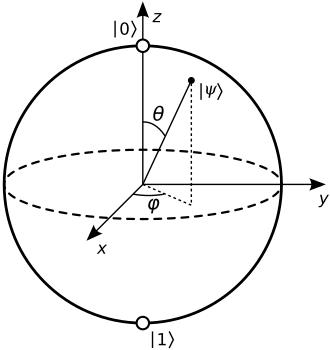
\includegraphics[width=0.3\textwidth]{img/Bloch/bloch_sphere.png}
        \caption{Esfera de Bloch. Obtenida de~\cite{wikiblochsphere}}\label{fig: bloch_sphere}
    \end{figure}

    Pudiendo representar todos los posibles estados de un qubit \( \ket{\psi} \) como un vector dentro de esta esfera. 
    Si nos fijamos en la expresión (\ref{eq: qubit_trigonometrico_esfera_bloch}) que acabamos de ver, vemos que hay un número complejo \( e^{i \varphi} \) de módulo uno, similar a una fase global. Sin embargo, esto no es una fase global, ya que para ello ha de multiplicar a todos los posibles estados del qubit, y vemos en este caso que solo aparece en el estado \( \ket{1} \), por lo que es una \textit{fase relativa}, y a diferencia de las fases globales que no cambian el significado físico del qubit, la fase relativa sí lo modifica. Esto es debido a que, aunque los coeficientes que acompañan a \( \ket{0} \) y \( \ket{1} \) sigan cumpliendo que su módulo al cuadrado sea uno, el vector representado en la esfera de Bloch es diferente, ya que puede variar el ángulo \( \varphi \).

    \vspace{5mm}

    Podemos pensar que aunque cambie la fase relativa no va a cambiar la probabilidad de obtener el estado \( \ket{0} \) o \( \ket{1} \) al medir el qubit. Esto se debe a que las mediciones se realizan normalmente sobre el eje \( Z \) y dicho vector estaría a la misma distancia de ambos polos de la esfera, manteniendo la probabilidad de obtener ambos estados \( \ket{0}, \ket{1} \) invariante, ya que la probabilidad de obtener un estado viene dada por el módulo al cuadrado de los coeficientes que los acompañan, como se puede apreciar en la expresión (\ref{eq: condicion_coeficientes_probabilidad_1}). Pero, ¿Y si cambiamos de base?
    
    \vspace{10mm}

    \subsection{Medición del Estado un Qubit}

    \vspace{5mm}

    Antes de hacer cambios de base, tenemos que tratar sobre las mediciones, las cuales ya hemos introducido en los párrafos anteriores y en esta pequeña sección vamos a profundizar sobre este tema. Como bien sabemos, un qubit puede estar en una superposición de \( \ket{0} \) y \( \ket{1} \) debido a las leyes de la mecánica cuántica, pero esto también establece que cuando vamos a leer el resultado de una operación, como al finalizar un algoritmo cuántico, este qubit colapsa a un único estado, de manera que obtenemos \( \ket{0} \) o bien \( \ket{1} \), cada uno con una cierta probabilidad, y esa probabilidad es el módulo al cuadrado de los coeficientes que acompañan a cada posible estado, como vimos en (\ref{eq: condicion_coeficientes_probabilidad_1}). Estos coeficientes se denominan amplitudes, y al tratarse de una probabilidad, la suma del módulo al cuadrado de las amplitudes ha de ser igual a uno. Vamos a ver esto con un ejemplo:

    \vspace{2.5mm}

    \begin{figure}[H]
        \small
        \centering
        \begin{minipage}{0.3\textwidth}
            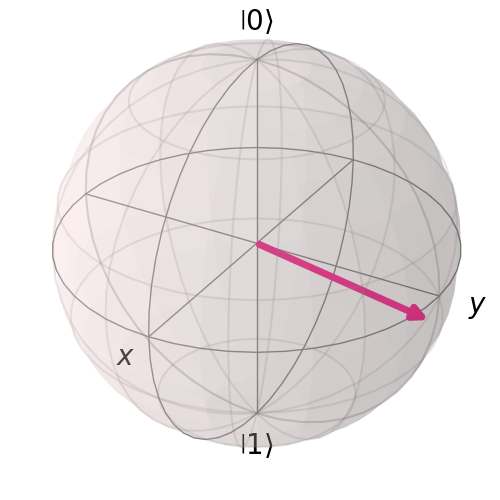
\includegraphics[width=\textwidth]{img/Bloch/bloch_measurement_example.png}  
            \caption{Medición de un Qubit.}\label{fig: bloch_ejemplo_medicion} 
        \end{minipage}
        \hfill
        \begin{minipage}{0.65\textwidth}
            Sea el siguiente qubit \( \ket{\psi} \):
            \begin{equation*}
                \ket{\psi} = \frac{1 + i \sqrt{3}}{3} \ket{0} + \frac{2 - i}{3} \ket{1}
            \end{equation*}
            La probabilidad de obtener el estado \( \ket{0} \) y el estado \( \ket{1} \) viene dada por 
            \begin{gather*}
                \left| \frac{1 + i \sqrt{3}}{3} \right| ^ {2} + \left| \frac{2 - i}{3} \right| ^ {2} = \left( \frac{1 + i \sqrt{3}}{3} \right) \left( \frac{1 - i \sqrt{3}}{3} \right) + \\[5pt]
                + \left( \frac{2 - i}{3} \right) \left( \frac{2 + i}{3} \right) = \frac{4}{9} + \frac{5}{9} = 1
            \end{gather*}
        \end{minipage}
    \end{figure}

    \vspace{2.5mm}

    Siendo la probabilidad de colapsar en \( \ket{0} \) de \( \frac{4}{9} \) y de \( \frac{5}{9} \) en el estado \( \ket{1} \). Esto lo podemos ver gráficamente si representamos el vector correspondiente al estado \( \ket{\psi} \) en la esfera de Bloch, ya que si nos fijamos en (\ref{fig: bloch_ejemplo_medicion}) podemos ver que \( \ket{\psi} \) está un poco más cercano al estado \( \ket{1} \) de dicha esfera, y esto se corresponde con una probabilidad mayor de obtener dicho estado, como hemos podido apreciar en el ejemplo anterior.

    \vspace{5mm}

    Una vez definida correctamente la medición de un qubit, podemos hablar más profundamente sobre el concepto de \textit{colapso} de un qubit. Cuando medimos un qubit, este colapsa a un estado como hemos visto anteriormente, que puede ser \( \ket{0} \) o \( \ket{1} \) según el ejemplo propuesto, de manera que el estado del qubit se vuelve completamente fijo al estado que ha colapsado, por lo que el qubit deja de estar en superposición, y es forzado a tomar un bando, en este caso \( \ket{0} \) o \( \ket{1} \). Esto hace que el estado del qubit esté ya completamente definido, de manera que si volvemos a medir el estado de \( \ket{\psi} \), obtendremos el estado al que ha colapsado con una probabilidad de 1.

    \vspace{5mm}

    Tomando el ejemplo anterior, supongamos que \( \ket{\psi} \) colapsa a \( \ket{1} \). La probabilidad de que \( \ket{\psi} \) haya colapsado en \( \ket{1} \) es de \( \frac{5}{9} \) según la explicación anterior, sin embargo, si medimos el qubit una segunda vez, es decir, después de que haya colapsado, la probabilidad de obtener otra vez el mismo estado \( \ket{1} \) es 1, mientras que la probabilidad de obtener \( \ket{0} \) es 0. Esto es debido a que el qubit ya ha colapsado a un estado, por lo que podemos concluir que las mediciones de los qubits afectan a su estado físico, dejando de estar en superposición e influyendo el resultado de las mediciones posteriores. Es por esto que, generalmente, vamos a realizar las mediciones de los diferentes qubits al final de un algoritmo cuántico.

    \vspace{10mm}





    \subsection{Cambio de Base}

    \vspace{5mm}

    Generalmente, vamos a realizar las mediciones en el eje \( Z \), ya que los polos de este eje son los estados \( \ket{0} \) y \( \ket{1} \), que representan la información clásica de un bit, la cual sabemos que puede ser 0 o 1, por lo que efectivamente, toda la información clásica, o mejor dicho, todo algoritmo clásico se puede realizar mediante un algoritmo cuántico, simplemente haciendo una adaptación de puertas lógicas a puertas cuánticas como ya veremos más adelante. 

    \vspace{5mm}

    Ya sabemos la razón por la que vamos a medir en la mayoría de los casos sobre el eje \( Z \), pero como podemos apreciar en la esfera de Bloch, tenemos infinitos ejes sobre los que podríamos hacer la medición, así que la única condición para escoger dos puntos como vectores base de nuestro espacio de Hilbert \( \mathcal{H} \) sobre el que estudiaremos el estado de nuestro qubit \( \ket{\psi} \), es que estos puntos sean completamente opuestos. Vamos a tomar como ejemplo los estados en el eje \( X \) e \( Y \), cuyos polos son \( \ket{+}, \ket{-} \) y \( \ket{i}, \ket{-i} \), respectivamente

    \begin{figure}[H]
        \centering
        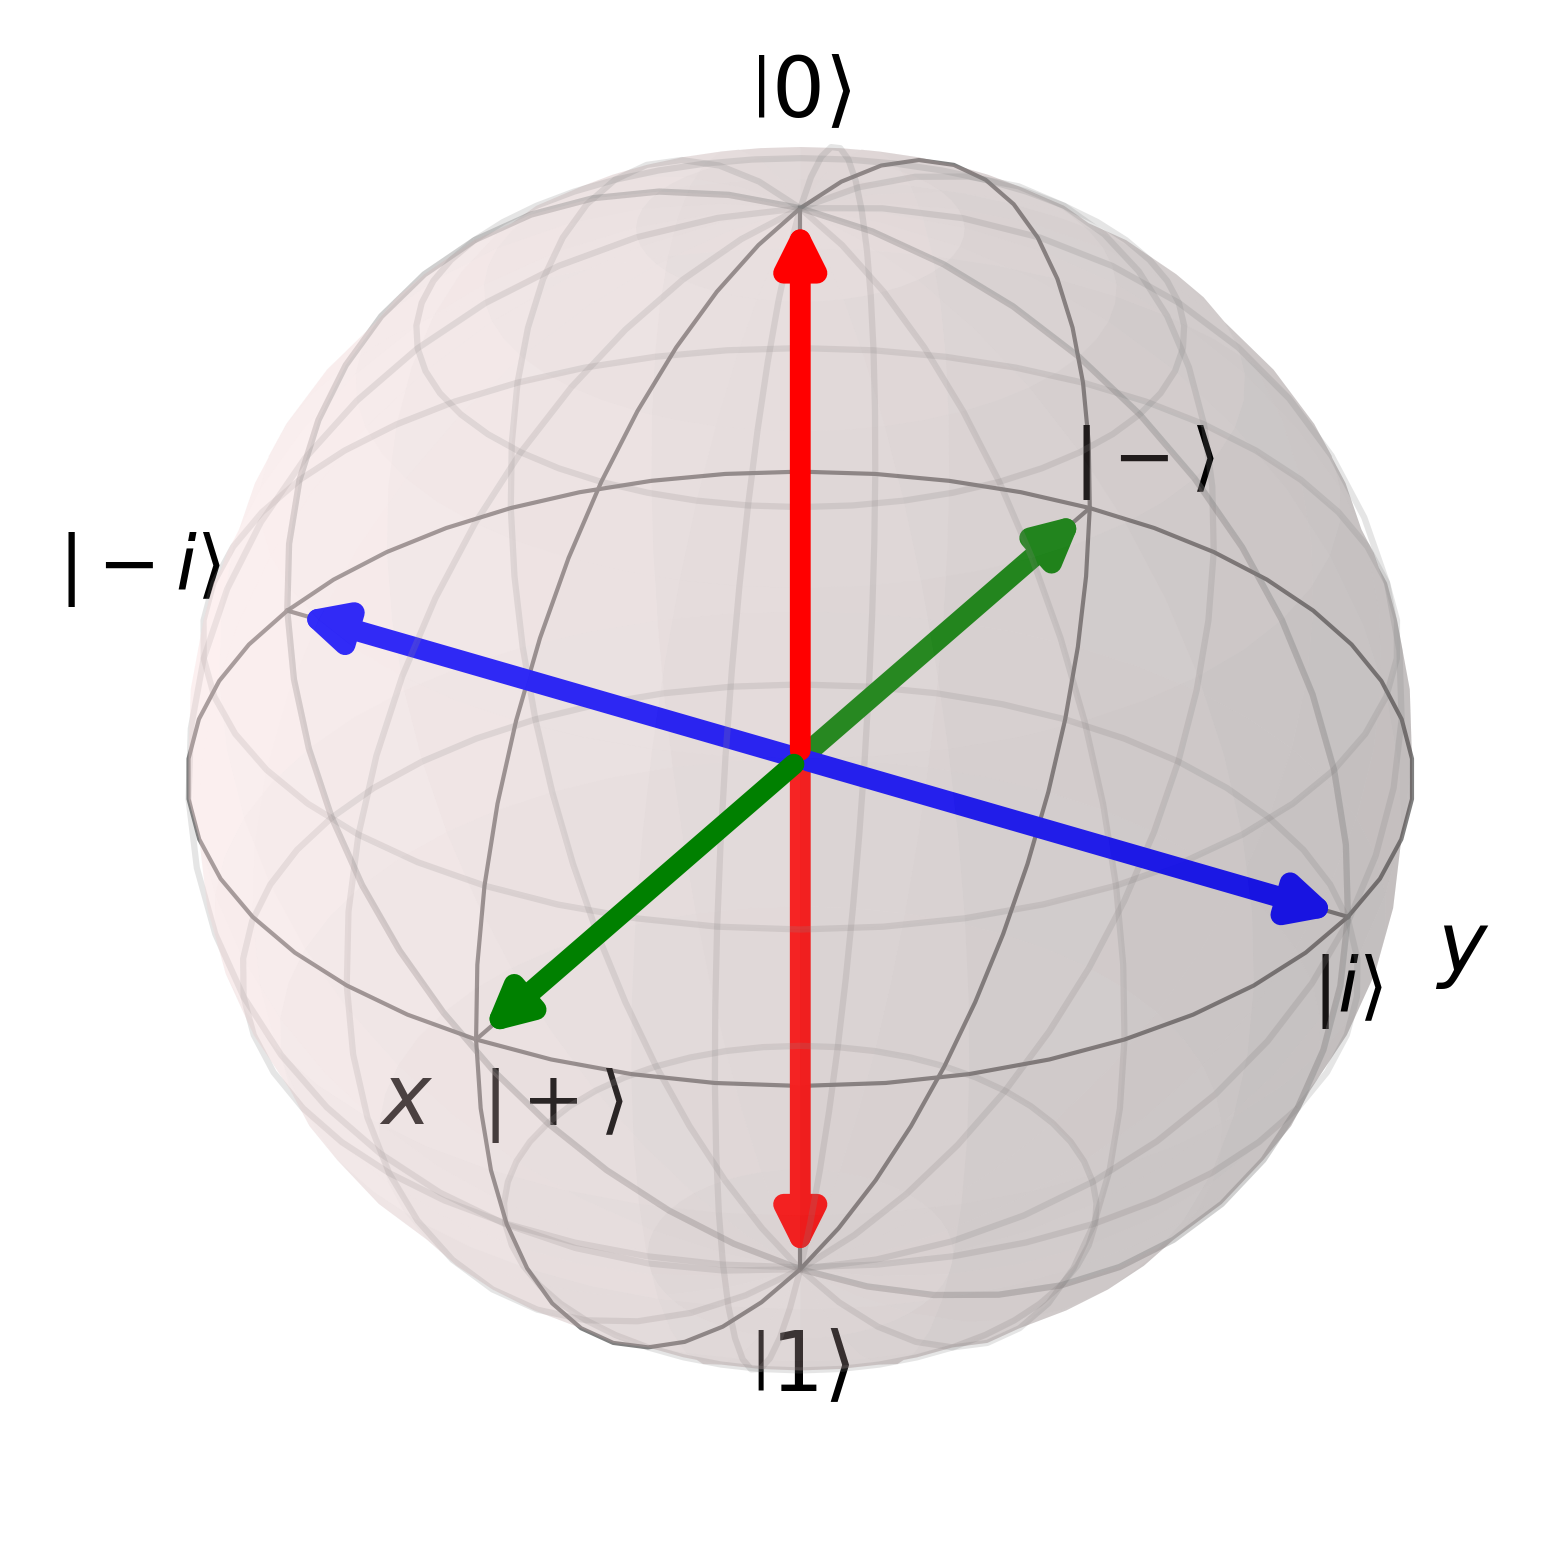
\includegraphics[width=0.3\textwidth]{img/Bloch/bloch_other_bases.png}
        \caption{Estados principales de la esfera de Bloch.}\label{fig: bloch_other_bases}
    \end{figure}

    Estos estados se pueden expresar en base a \( \ket{0} \) y \( \ket{1} \):

    \begin{align}
        \label{eq: estados_eje_x_y}
        \ket{+} &= \frac{1}{\sqrt{2}} \left( \ket{0} + \ket{1} \right) \\[10pt]
        \ket{-} &= \frac{1}{\sqrt{2}} \left( \ket{0} - \ket{1} \right) \\[10pt]
        \ket{i} &= \frac{1}{\sqrt{2}} \left( \ket{0} + i\ket{1} \right) \\[10pt]
        \ket{-i} &= \frac{1}{\sqrt{2}} \left( \ket{0} - i\ket{1} \right)
    \end{align}

    \vspace{2.5mm}

    Y su representación la podemos ver reflejada en (\ref{fig: bloch_other_bases}). Estos estados sabemos que están en superposición ya que no se encuentran en \( \ket{0} \) o \( \ket{1} \), de hecho, están justamente en el punto medio entre \( \ket{0} \) y \( \ket{1} \), por lo que la probabilidad de obtener \( \ket{0} \) o \( \ket{1} \) es exactamente la misma (\( \frac{1}{2} \)) si nuestro qubit \( \ket{\psi} \) se encuentra en uno de los estados en (\ref{eq: estados_eje_x_y}). No obstante, para poder realizar el cambio de base, necesitamos expresar los estados \( \ket{0} \) y \( \ket{1} \) en función de la base a la que queramos aplicar el cambio. Comencemos por \( \ket{+} \) y \( \ket{-} \):

    \begin{align}
        \ket{+} + \ket{-} &= \frac{1}{\sqrt{2}} \left( \ket{0} + \ket{1} \right) + \frac{1}{\sqrt{2}} \left( \ket{0} - \ket{1} \right) = \frac{2}{\sqrt{2}} \ket{0} = \sqrt{2} \ket{0} \nonumber \\[5pt] 
        & \implies \ \boxed{\ket{0} = \frac{1}{\sqrt{2}} \left( \ket{+} + \ket{-} \right)} 
        \label{eq: estado_0_en_funcion_mas_menos}
    \end{align}
    \begin{align}
        \ket{+} - \ket{-} &= \frac{1}{\sqrt{2}} \left( \ket{0} + \ket{1} \right) - \frac{1}{\sqrt{2}} \left( \ket{0} - \ket{1} \right) = \frac{2}{\sqrt{2}} \ket{1} = \sqrt{2} \ket{1} \nonumber \\[5pt]
        & \implies \ \boxed{\ket{1} = \frac{1}{\sqrt{2}} \left( \ket{+} - \ket{-} \right)}
        \label{eq: estado_1_en_funcion_mas_menos}
    \end{align}

    \vspace{5mm}

    Y esto está muy relacionado con la \textit{puerta de Hadamard}, la cual es una de las puertas cuánticas de un qubit más importantes, como veremos en la siguiente sección. Volviendo a retomar el ejemplo (\ref{fig: bloch_ejemplo_medicion}), vamos a aplicar el cambio a la base \( B_{H} = \left\{ \ket{+}, \ket{-} \right\}\) y ver como afecta esto al estado de nuestro qubit \( \ket{\psi} \). Aplicando dicho cambio, nos queda lo siguiente

    \vspace{2.5mm}

    \begin{figure}[H]
        \small
        \centering
        \begin{minipage}{0.65\textwidth}
            \begin{gather*}
                \ket{\psi} = \frac{1 + i \sqrt{3}}{3} \ket{0} + \frac{2 - i}{3} \ket{1} = \frac{1 + i \sqrt{3}}{3 \sqrt{2}} \left( \ket{+} + \ket{-} \right) + \frac{2 - i}{3 \sqrt{2}} \left( \ket{+} - \ket{-} \right) = \\[5pt]
                = \frac{3 + \left( \sqrt{3} - 1 \right) i}{3 \sqrt{2}} \ket{+} - \frac{1 - \left( \sqrt{3} + 1 \right) i}{3 \sqrt{2}} \ket{-}
            \end{gather*}
            Y la probabilidad de obtener \( \ket{+} \) y \( \ket{-} \) es 
            \begin{align*}
                \ket{+} \ &\longrightarrow \ \left| \ \frac{3 + \left( \sqrt{3} - 1 \right) i}{3 \sqrt{2}} \ \right| ^ {2} = \frac{9 + \left( \sqrt{3} - 1\right) ^ {2}}{18} \approx 0.53 \\[10pt]
                \ket{-} \ &\longrightarrow \ \left| \ \frac{1 - \left( \sqrt{3} + 1 \right) i}{3 \sqrt{2}} \ \right| ^ {2} = \frac{1 + \left( \sqrt{3} + 1\right) ^ {2}}{18} \approx 0.47
            \end{align*}
        \end{minipage}
        \hfill
        \begin{minipage}{0.3\textwidth}
            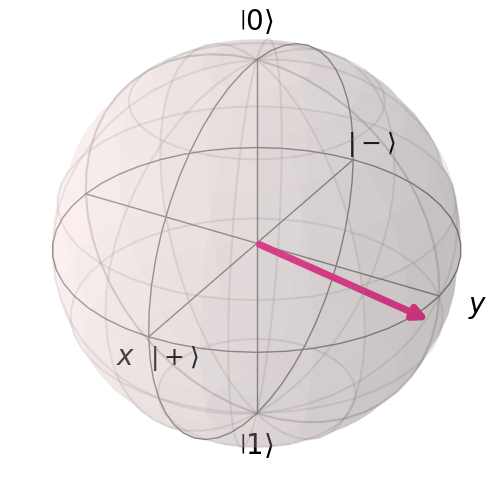
\includegraphics[width=\textwidth]{img/Bloch/bloch_change_basis_example.png} 
            \caption{Cambio a la base $ \{ \ket{+}, \ket{-} \} $.}\label{fig: bloch_ejemplo_medicion_2}  
        \end{minipage}
    \end{figure}

    \vspace{2.5mm}

    Podemos ver que esto tiene sentido, ya que el vector que representa el estado de \( \ket{\psi} \) se encuentra ligeramente más próximo al estado \( \ket{+} \) que a \( \ket{-} \), por lo que es lógico obtener una probabilidad en \( \ket{+} \) ligeramente mayor que en \( \ket{-} \), aunque esto no quiere decir que vaya a colapsar siempre a \( \ket{+} \), significa que si midiéramos varios qubits en el mismo estado que \( \ket{\psi} \), por estadísitica, obtendríamos normalmente mayor número de colapsos en \( \ket{+} \), aunque no siempre va a colapsar en \( \ket{+} \) por tener una probabilidad mayor.

    \vspace{5mm}

    De la misma manera que en (\ref{eq: estado_0_en_funcion_mas_menos}) y (\ref{eq: estado_1_en_funcion_mas_menos}), podemos expresar \( \ket{0} \) y \( \ket{1} \) en función de \( \ket{i} \) y \( \ket{-i} \), obteniendo que

    \begin{equation}
        \ket{0} = \frac{1}{\sqrt{2}} \left( \ket{i} + \ket{-i} \right), \quad \ket{1} = \frac{-i}{\sqrt{2}} \left( \ket{i} - \ket{-i} \right) 
        \label{eq: estado_0_y_1_en_funcion_i_menosi}
    \end{equation}

    \vspace{5mm}

    En este caso la diferencia entre ambas probabilidades va a ser mucho mayor, ya que \( \ket{\psi} \) está muy próximo a \( \ket{i} \) en la esfera de Bloch, por lo que la probabilidad de obtener \( \ket{i} \) será muy cercana a uno, y en caso contrario, la probabilidad de obtener \( \ket{-i} \) será prácticamente nula.

    \vspace{2.5mm}

    \begin{figure}[H]
        \small
        \centering
        \begin{minipage}{0.3\textwidth}
            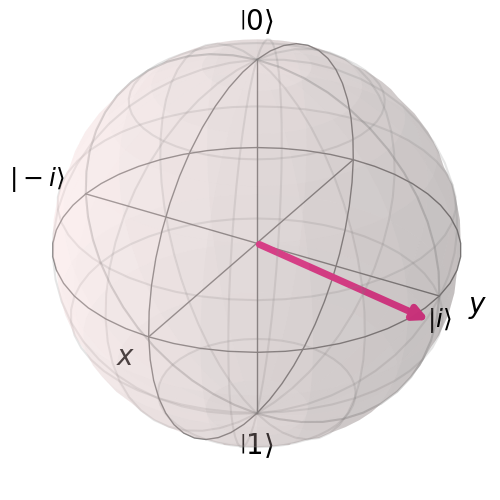
\includegraphics[width=\textwidth]{img/Bloch/bloch_change_basis_example_2.png}  
            \caption{Cambio a la base $ \{ \ket{i}, \ket{-i} \} $.}\label{fig: bloch_ejemplo_medicion_3} 
        \end{minipage}
        \hfill
        \begin{minipage}{0.65\textwidth}
            \begin{gather*}
                \ket{\psi} = \frac{1 + i \sqrt{3}}{3} \ket{0} + \frac{2 - i}{3} \ket{1} = \frac{1 + \sqrt{3}i}{3 \sqrt{2}} \left( \ket{i} + \ket{-i} \right) - \\[5pt]
                - \frac{1 + 2i}{3 \sqrt{2}} \left( \ket{i} - \ket{-i} \right) =  \frac{\left( \sqrt{3} - 2 \right)i}{3 \sqrt{2}} \ket{i} + \frac{2 + \left( \sqrt{3} + 2 \right) i}{3 \sqrt{2}} \ket{-i}
            \end{gather*}
            Y la probabilidad de obtener \( \ket{i} \) y \( \ket{-i} \) es
            \begin{align*}
                \ket{i} \ &\longrightarrow \ \left| \ \frac{\left( \sqrt{3} - 2 \right) i}{3 \sqrt{2}} \ \right| ^ {2} = \frac{\left( \sqrt{3} - 2 \right) ^ {2}}{18} \approx 0.004 \\[10pt]
                \ket{-i} \ &\longrightarrow \ \left| \ \frac{2 + \left( \sqrt{3} + 2 \right) i}{3 \sqrt{2}} \ \right| ^ {2} = \frac{4 + \left( \sqrt{3} + 2 \right) ^ {2}}{18} \approx 0.996
            \end{align*}
        \end{minipage}
    \end{figure}

    \vspace{2.5mm}

    Perfecto, vemos que el resultado es el esperado. Ahora, estamos en condiciones de explicar la fase relativa correctamente. Al final de (\ref{sec: el_qubit}), explicamos que una fase global no modifica el estado físico de un qubit, pero dejamos un poco abierta la fase relativa. Vamos a volver a trabajar sobre el estado de un qubit puro definido en (\ref{eq: qubit_trigonometrico_esfera_bloch}), definiendo las probabilidades de medir \( \ket{\psi} \) sobre el eje \( Z \) y posteriormente sobre el eje \( X \), y nos vamos a dar cuenta que las probabilidades no coinciden, concluyendo en que una fase relativa sí que modifica el estado físico de un qubit, a diferencia de una fase global. Comencemos por la probabilidad de obtener \( \ket{0} \) y \( \ket{1} \)

    \begin{equation*}
        \ket{\psi} = \cos \left( \frac{\theta}{2} \right) \ket{0} + e^{i \varphi} \sin \left( \frac{\theta}{2} \right) \ket{1}
    \end{equation*}
    \begin{align*}
        \ket{0} \ &\longrightarrow \ \left| \cos \left( \frac{\theta}{2} \right) \right| ^ {2} = \cos^{2} \left( \frac{\theta}{2} \right) \\[10pt]
        \ket{1} \ &\longrightarrow \ \left| e^{i \varphi} \sin \left( \frac{\theta}{2} \right) \right| ^ {2} = \left( \cos \left( \frac{\theta}{2} \right) + i \sin \left( \frac{\theta}{2} \right) \right) \left( \cos \left( \frac{\theta}{2} \right) - i \sin \left( \frac{\theta}{2} \right) \right) \sin^{2} \left( \frac{\theta}{2} \right) = \sin^{2} \left( \frac{\theta}{2} \right)
    \end{align*}

    \vspace{2.5mm}

    Ahora, haciendo el cambio de base a \( \left\{ \ket{0}, \ket{1} \right\} \)
    \begin{equation*}
        \ket{\psi} = \frac{1}{\sqrt{2}} \cos \left( \frac{\theta}{2} \right) \left( \ket{+} + \ket{-} \right) + \frac{1}{\sqrt{2}} + \frac{1}{\sqrt{2}} e^{i \varphi} \sin \left( \frac{\theta}{2} \right) \left( \ket{+} - \ket{-} \right) = 
    \end{equation*}
    \begin{equation*}
        = \left[ \frac{1}{\sqrt{2}} \cos \left( \frac{\theta}{2} \right) + \frac{1}{\sqrt{2}} e^{i \varphi} \sin \left( \frac{\theta}{2} \right) \right] \ket{+} + \left[ \frac{1}{\sqrt{2}} \cos \left( \frac{\theta}{2} \right) - \frac{1}{\sqrt{2}} e^{i \varphi} \sin \left( \frac{\theta}{2} \right) \right] \ket{-} 
    \end{equation*}

    \vspace{2.5mm}

    Vemos que las probabilidades no son las mismas que con la base anterior:
    \begin{align*}
        \ket{+} \ &\longrightarrow \ \left| \frac{1}{\sqrt{2}} \cos \left( \frac{\theta}{2} \right) + \frac{1}{\sqrt{2}} e^{i \varphi} \sin \left( \frac{\theta}{2} \right) \right| ^ {2} = \frac{1}{2} \left[ \cos \left( \frac{\theta}{2} \right) + \sin \left( \frac{\theta}{2} \right)\right] ^ {2} \\[10pt]
        \ket{-} \ &\longrightarrow \ \left| \frac{1}{\sqrt{2}} \cos \left( \frac{\theta}{2} \right) - \frac{1}{\sqrt{2}} e^{i \varphi} \sin \left( \frac{\theta}{2} \right) \right| ^ {2} = \frac{1}{2} \left[ \cos \left( \frac{\theta}{2} \right) - \sin \left( \frac{\theta}{2} \right)\right] ^ {2}
    \end{align*}

    \vspace{5mm}

    Por lo que hemos comprobado que una fase relativa no altera el estado de un qubit \( \ket{\psi} \) en el eje \( Z \), sino que lo hace en el plano azimutal, de manera que al medir el estado de \( \ket{\psi} \) en otra base como \( \{ \ket{+}, \ket{-} \} \), la probabilidad de colapso cambia. Esto no sucede cuando aplicamos una fase global.

    \vspace{10mm}


    


    \subsection{Puertas Cuánticas}\label{sec: puertas_cuanticas}

    \vspace{5mm}

    Habiendo introducido la unidad de información cuántica y sus respectivas mediciones sobre los ejes \( X \), \( Y \) y \( Z \), estamos ya en condiciones de estudiar las puertas cuánticas. Así como las puertas lógicas en computación clásica son capaces de modificar la información que reside en los distintos bits, las puertas cuánticas actúan sobre el estado físico de los respectivos qubits, siguiendo las leyes de la mecánica cuántica como hemos visto hasta ahora, de manera que se consigue modificar el estado de un qubit \( \ket{\psi} \) como resultado de una operación, por ejemplo, desencriptar las claves públicas y privadas de un cifrado de información, como veremos más adelante.
    
    \vspace{5mm}

    Estas puertas cuánticas, las podemos representar como matrices, aprovechando todo el álgebra lineal que llevamos impartido hasta ahora. Realmente, pudimos haber representado el estado de un qubit \( \ket{\psi} \) en la sección anterior como un vector columna, aprovechando la representación matricial de \( \ket{0} \) y \( \ket{1} \) que sigue como

    \begin{equation}
        \ket{0} = \begin{pmatrix}
            1 \\
            0
        \end{pmatrix}
        , \quad \ket{1} = \begin{pmatrix}
            0 \\
            1
        \end{pmatrix}
    \end{equation}

    \vspace{2.5mm}

    Si tomamos el estado de un qubit puro que definimos en (\ref{eq: combinacion_lineal_estados_1_qubit}), vemos que podemos definir el estado de un qubit cualquiera \( \ket{\psi} \) como un vector columna de dimensión \( 2^{N} \), siendo \( N \) el número de qubits de nuestro computador cuántico, por lo que para un sistema cuántico de un único qubit tenemos el siguiente vector:

    \begin{equation}
        \ket{\psi} = \alpha \ket{0} + \beta \ket{1} = \alpha \begin{pmatrix}
        1 \\
        0
        \end{pmatrix} + \beta \begin{pmatrix}
        0 \\
        1
        \end{pmatrix} = \begin{pmatrix}
        \alpha \\
        \beta
        \end{pmatrix}
        \label{eq: vector_sistema_un_qubit}
    \end{equation}

    \vspace{2.5mm}

    De esta manera, podemos expresar el estado de cualquier qubit como un vector columna de dimensión 2, y ya veremos la generalización de esta representación vectorial para \( N \) qubits en la siguiente sección (\ref{sec: multiples_qubits}). Por otra parte, vamos ya a afrontar las puertas cuánticas, las cuales no son más que operadores sobre un espacio de Hilbert \( \mathcal{H} \) que transforman el estado de un qubit en otro estado diferente, como vimos en (\ref{eq: operador_espacio_hilbert}):

    \begin{equation*}
        \hat{A} \ket{\psi} \overset{\hat{A}}{\longrightarrow} \ket{\psi '}, \qquad \ket{\psi}, \ket{\psi '} \in \mathcal{H}
    \end{equation*}

    \vspace{2.5mm}

    Para estos operadores ser bautizados como puertas cuánticas, han de satisfacer unas ciertas condiciones. La primera es la condición de linealidad, la cual establece que

    \begin{equation}
        U \left( \alpha \ket{0} + \beta \ket{1} \right) = \alpha U \ket{0} + \beta U \ket{1}
        \label{eq: linealidad_puertas_cuanticas}
    \end{equation}

    \vspace{2.5mm}

    La segunda es que la probabilidad total de los estados a obtener en una medición ha de seguir manteniéndose uno, como vimos en el capítulo anterior en (\ref{eq: condicion_coeficientes_probabilidad_1})

    \begin{equation*}
        | \alpha | ^ {2} + | \beta | ^ {2} = 1
    \end{equation*}

    \vspace{2.5mm}

    Para ver qué tipo de matrices satisfacen esta propiedad, vamos a apoyarnos en el conjugado hermítico. Sea la siguiente puerta cuántica \( U \):

    \begin{equation*}
        U = \begin{pmatrix}
            a & c \\
            b & d
        \end{pmatrix}
    \end{equation*}

    \vspace{2.5mm}

    Si la aplicamos sobre un qubit \( \ket{\psi} \), nos queda como resultado un qubit diferente, el cual denotaremos como \( \ket{U \psi} \)

    \begin{equation}
        U \ket{\psi} = \begin{pmatrix}
            a & c \\
            b & d
        \end{pmatrix} \begin{pmatrix}
            \alpha \\
            \beta
        \end{pmatrix} = \begin{pmatrix}
            a \alpha + c \beta \\
            b \alpha + d \beta
        \end{pmatrix} = \ket{U \psi}
    \label{eq: puerta_cuantica_vector_aplicado}
    \end{equation}

    \vspace{2.5mm}

    Si ahora consideramos el conjugado hermítico de \( \ket{U \psi} \), el cual definimos en la introducción de los espacios de Hilbert \( \mathcal{H} \) en (\ref{eq: conjugado_hermitico}), tenemos que

    \begin{gather}
        \bra{U \psi} = \begin{pmatrix}
            a^{*} \alpha^{*} + c^{*} \beta^{*} & b^{*} \alpha^{*} + d^{*} \beta^{*} 
        \end{pmatrix} = \begin{pmatrix}
            \alpha^{*} & \beta^{*}
        \end{pmatrix} \begin{pmatrix}
            a^{*} & d^{*} \\
            c^{*} & d^{*}
        \end{pmatrix} = \nonumber \\[5pt]
        = \begin{pmatrix}
            \alpha^{*} & \beta^{*}
        \end{pmatrix} \begin{pmatrix}
            a & c \\
            b & d
        \end{pmatrix} ^ {\dagger} = \bra{\psi} U^{\dagger}
    \label{eq: puerta_cuantica_conjugado_hermitico}
    \end{gather}

    \vspace{2.5mm}

    Entonces, apoyándonos en las propiedades que acabamos de ver (\ref{eq: puerta_cuantica_vector_aplicado}) y (\ref{eq: puerta_cuantica_conjugado_hermitico}), obtenemos finalmente la segunda condición que estamos buscando. Esto lo hacemos viendo que el producto escalar de \( \ket{U \psi} \) sobre sí mismo, es decir, la proyección de \( \ket{U \psi} \) sobre sí mismo, es igual a 1:
    \begin{align}
        \braket{U \psi \ | \ U \psi} &= 1 \nonumber \\[10pt]
        \braket{\psi | U^{\dagger} U | \psi} &= \braket{\psi \ | \ \psi} \nonumber \\[10pt]
        U^{\dagger} U &= I
        \label{eq: puertas_cuanticas_unitarias}
    \end{align}

    Y las matrices que satisfacen esta última propiedad (\ref{eq: puertas_cuanticas_unitarias}) se conocen como \textit{unitarias}, y podemos afirmar algo muy importante, y es que toda matriz unitaria es una puerta cuántica, y toda puerta cuántica es una matriz unitaria. Además, como hemos podido ver en (\ref{eq: puertas_cuanticas_unitarias}), \( U^{\dagger} \) es la matriz inversa de \( U \), ya que el producto de estas dos matrices da como resultado la matriz identidad \( I \), por lo que toda puerta cuántica \( U \) es reversible, y su matriz inversa es su conjugado hermítico \( U^{\dagger} \), de manera que si aplicamos una puerta cuántica \( U \) sobre un qubit \( \ket{\psi} \), podemos volver al estado original de \( \ket{\psi} \) aplicando \( U^{\dagger} \)

    \begin{equation*}
        U^{\dagger} U \ket{\psi} = U U^{\dagger} \ket{\psi} = I \ket{\psi} = \ket{\psi}
    \end{equation*}

    \vspace{2.5mm}

    Esta última condición tiene mucho que ver con que las puertas cuánticas tienen que ser reversibles, es decir, siempre hemos de saber de que estado proviene el resultado. Para ver esto mejor, vamos a apoyarnos en las puertas lógicas clásicas, en este caso la puerta \textit{NOT}, cuya tabla de verdad es

    \begin{table}[h!]
        \centering
        \begin{tabular}{|c|c|}
            \hline
            A & B \\
            \hline
            0 & 1 \\
            1 & 0 \\
            \hline
        \end{tabular}
        \caption{Puerta lógica NOT.}
        \label{table: puerta_clasica_not}
    \end{table}

    Si obtenemos el resultado \( B = 1 \), sabemos que el bit antes de aplicar la puerta era \( 0 \), y si obtenemos \( B = 0 \), no queda otra opción que el bit fuese \( 1 \), esto lo podemos representar como una matriz:
    
    \begin{equation*}
        \begin{array}{l}
            \ket{0} \rightarrow 1 \\
            \ket{1} \rightarrow 0  
        \end{array}
        \left\}
        \quad
        \text{NOT} =
        \begin{pmatrix}
            0 & 1 \\
            1 & 0
        \end{pmatrix}
    \end{equation*}

    \vspace{2.5mm}

    Y esta matriz vemos que es unitaria, ya que su matriz conjugada transpuesta por ella misma es la identidad \( I \)

    \begin{equation*}
        \begin{pmatrix}
            0 & 1 \\
            1 & 0
        \end{pmatrix} \begin{pmatrix}
            0 & 1 \\
            1 & 0
        \end{pmatrix} ^ {\dagger} = \begin{pmatrix}
            0 & 1 \\
            1 & 0
        \end{pmatrix} \begin{pmatrix}
            0 & 1 \\
            1 & 0
        \end{pmatrix} = I
    \end{equation*}

    \vspace{2.5mm}

    Por lo que la puerta clásica \textit{NOT} es una puerta cuántica perfectamente válida, la cual explicaremos en el siguiente apartado. Para ver el caso contrario, vamos a suponer la puerta clásica cuyo resultado es siempre 1:
    
    \begin{table}[h!]
        \centering
        \begin{tabular}{|c|c|}
            \hline
            A & B \\
            \hline
            0 & 1 \\
            1 & 1 \\
            \hline
        \end{tabular}
        \caption{Puerta lógica clásica constante a 1.}
        \label{table: puerta_clasica_todo_1}
    \end{table}

    Y  podemos verificar que la matriz que representa a esta puerta no es unitaria
        
    \begin{equation*}
        \begin{pmatrix}
            0 & 0 \\
            1 & 1
        \end{pmatrix} \begin{pmatrix}
            0 & 0 \\
            1 & 1
        \end{pmatrix} ^ {\dagger} = \begin{pmatrix}
            0 & 0 \\
            1 & 1
        \end{pmatrix} \begin{pmatrix}
            0 & 1 \\
            0 & 1
        \end{pmatrix} =  \begin{pmatrix}
            0 & 0 \\
            0 & 1
        \end{pmatrix} \neq I
    \end{equation*}

    \vspace{2.5mm}

    Por lo que la puerta (\ref{table: puerta_clasica_todo_1}) no es una puerta cuántica. Este pequeño nos ayuda a entender mejor que toda puerta lógica clásica reversible tiene su contrapartida en computación cuántica, y el significado físico de estas puertas cuánticas lo vamos a ver a continuación con las puertas cuánticas de 1 qubit más importantes.

    \vspace{10mm}





    \subsection{Puertas Cuánticas de 1 Qubit}\label{subsection: puertas_cuanticas_de_1_qubit}

    \vspace{5mm}

    Una vez explicadas las condiciones que ha de cumplir una puerta cuántica, que son la condición de linealidad (\ref{eq: linealidad_puertas_cuanticas}) y que ha de ser unitaria, como vimos en (\ref{eq: puertas_cuanticas_unitarias}), vamos a tomar como ejemplo la puerta \textit{NOT} clásica, que tiene su contrapartida cuántica, la cual se suele denotar como \textit{X}, ya que cumple con los requisitos propuestos anteriormente, de manera que un qubit en el estado \( \ket{0} \) pasa a \( \ket{1} \) y viceversa:

    \begin{equation*}
        & X \ket{\psi} = \alpha X \ket{0} + \beta  X \ket{1} = \alpha \begin{pmatrix}
            0 & 1 \\
            1 & 0 
        \end{pmatrix} \begin{pmatrix}
            1 \\
            0
        \end{pmatrix} + \beta \begin{pmatrix}
            0 & 1 \\
            1 & 0 
        \end{pmatrix} \begin{pmatrix}
            0 \\ 
            1
        \end{pmatrix} = \alpha \begin{pmatrix}
            0 \\
            1
        \end{pmatrix} + \beta \begin{pmatrix}
            1 \\
            0
        \end{pmatrix} = \beta \ket{0} + \alpha \ket{1} 
    \end{equation*}

    \vspace{2.5mm}

    De esta manera, si aplicamos la puerta \textit{X} sobre un qubit \( \ket{\psi} \) que se encuentra en el estado \( \ket{0} \), esta puerta rota el estado del qubit \( \ket{\psi} \) al estado \( \ket{1} \)

    \vspace{2.5mm}

    \begin{figure}[H]
        \centering
        \begin{subfigure}[t]{0.45\textwidth}
            \centering
            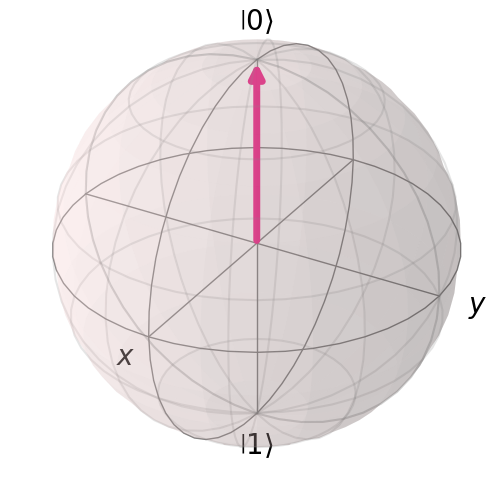
\includegraphics[width=0.675\textwidth]{img/Bloch/bloch_state_0.png}
            \caption{Estado $|0\rangle$ en la esfera de Bloch.}
        \end{subfigure}
        \scalebox{2}{\(\overset{X}{\longrightarrow}\)}
        \begin{subfigure}[t]{0.45\textwidth}
            \centering
            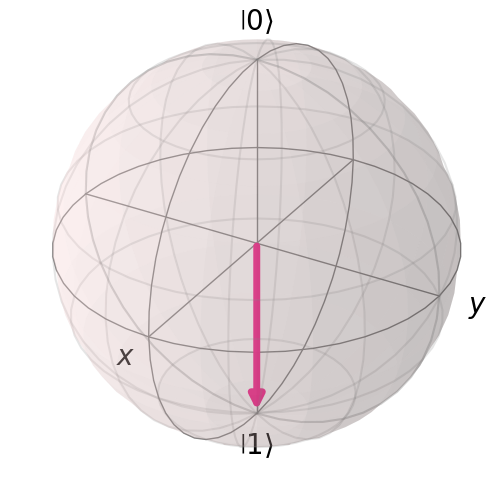
\includegraphics[width=0.675\textwidth]{img/Bloch/bloch_state_1.png}
            \caption{Estado $|1\rangle$ en la esfera de Bloch.}
        \end{subfigure}
    \end{figure}

    \vspace{2.5mm}

    Y esto ocurre también para el caso contrario. Esta puerta \textit{X} es una de las \textit{puertas de Pauli}, en concreto sobre el eje X, como su propio nombre indica, y también podemos definir las puertas de Pauli para el eje \textit{Y} y \textit{Z} de la esfera de Bloch, de la siguiente manera

    \begin{equation}
        X = \begin{pmatrix}
            0 & 1 \\
            1 & 0 
        \end{pmatrix}, \qquad Y = \begin{pmatrix}
            0 & -i \\
            i & 0
        \end{pmatrix}, \qquad Z = \begin{pmatrix}
            1 & 0 \\
            0 & -1
        \end{pmatrix}
        \label{eq: puertas_pauli}
    \end{equation}

    \vspace{2.5mm}

    Estas \textit{puertas de Pauli}, y de hecho, toda puerta cuántica de un único qubit representa una rotación de \( \ket{\psi} \) en la esfera de Bloch, esto es lógico ya que, como vimos anteriormente, toda puerta cuántica es un operador lineal que actúa sobre un qubit \( \ket{\psi} \), de manera que cambiamos el estado de dicho qubit \( \ket{\psi} \) a otro estado diferente \( \ket{\psi'} \), cuya norma sigue siendo la unidad, por lo que podemos visualizar muy bien la rotación en la esfera de Bloch. Así, las puertas de Pauli que acabamos de ver en (\ref{eq: puertas_pauli}) son rotaciones de \( \pi \) radianes sobre uno de los ejes de la esfera de Bloch. Veamos como actúa \textit{Y} sobre \( \ket{0} \):

    \begin{equation*}
        Y \ket{\psi} = \begin{pmatrix}
            0 & -i \\
            i & 0
        \end{pmatrix} \begin{pmatrix}
            1 \\
            0
        \end{pmatrix} = \begin{pmatrix}
            0 \\
            i
        \end{pmatrix} = i \begin{pmatrix}
            0 \\
            1
        \end{pmatrix} = i \ket{1}
    \end{equation*}

    \vspace{2.5mm}

    Y esto es el estado \( \ket{1} \) multiplicado por una fase global, en este caso \( i \), por lo que podemos eliminar la fase global, ya que esta no altera el significado físico de \( \ket{1} \), dándose por realizada la rotación esperada sobre el eje \textit{Y}

    \vspace{2.5mm}

    \begin{figure}[H]
        \centering
        \begin{subfigure}[t]{0.45\textwidth}
            \centering
            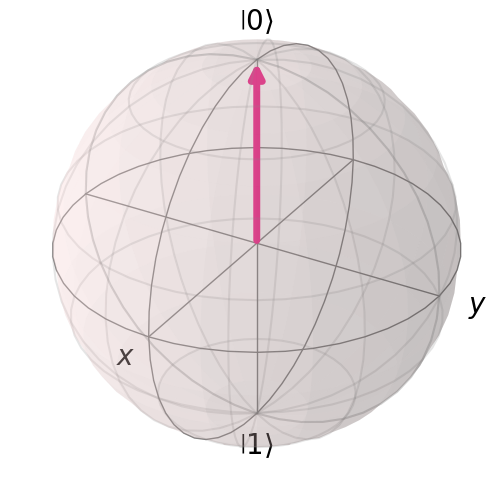
\includegraphics[width=0.675\textwidth]{img/Bloch/bloch_state_0.png}
        \end{subfigure}
        \scalebox{2}{\(\overset{Y}{\longrightarrow}\)}
        \begin{subfigure}[t]{0.45\textwidth}
            \centering
            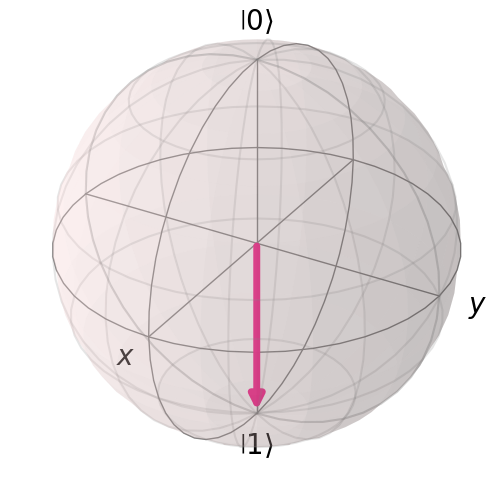
\includegraphics[width=0.675\textwidth]{img/Bloch/bloch_state_1.png}
        \end{subfigure}
    \end{figure}

    \vspace{2.5mm}

    Vamos a tomar como último ejemplo la puerta \textit{Z}, de manera que si la aplicamos sobre un qubit en \( \ket{0} \)
    el estado del qubit no cambia, ya que estamos aplicando una rotación sobre el eje \textit{Z}:

    \begin{equation*}
        Z \ket{0} = \begin{pmatrix}
            1 & 0 \\
            0 & -1
        \end{pmatrix} \begin{pmatrix}
            1 \\
            0
        \end{pmatrix} = \begin{pmatrix}
            1 \\
            0
        \end{pmatrix} = \ket{0}
    \end{equation*}

    \vspace{2.5mm}

    Como habíamos presupuesto anteriormente. A partir de estas puertas podemos crear todas las demás puertas cuánticas de 1 qubit. Vamos definir una puerta muy importante, la cual es una rotación sobre el eje \( X + Z \), que la podemos obtener únicamente sumando las puertas de Pauli \textit{X} y \textit{Z}

    \begin{equation*}
        X + Z = \begin{pmatrix}
            0 & 1 \\
            1 & 0 
        \end{pmatrix} + \begin{pmatrix}
            1 & 0 \\
            0 & -1
        \end{pmatrix} = \begin{pmatrix}
            1 & 1 \\
            1 & -1
        \end{pmatrix}
    \end{equation*}

    \vspace{2.5mm}

    Pero si nos fijamos esta matriz no es unitaria, ya que

    \begin{equation*}
        \begin{pmatrix}
            1 & 1 \\
            1 & -1
        \end{pmatrix} \begin{pmatrix}
            1 & 1 \\
            1 & -1
        \end{pmatrix} ^ {\dagger} = \begin{pmatrix}
            1 & 1 \\
            1 & -1
        \end{pmatrix} \begin{pmatrix}
            1 & 1 \\
            1 & -1
        \end{pmatrix} = \begin{pmatrix}
            2 & 0 \\
            0 & 2
        \end{pmatrix} = 2 \ I \neq I
    \end{equation*}

    \vspace{2.5mm} 

    Para que sea unitaria hemos de multiplicar la matriz por \( \frac{1}{\sqrt{2}} \), obteniendo así una nueva puerta cuántica, la cual suele representarse con \textit{H}:

    \begin{equation}
        H = \frac{1}{\sqrt{2}} \begin{pmatrix}
            1 & 1 \\
            1 & -1
        \end{pmatrix}
        \label{eq: puerta_hadamard}
    \end{equation}

    \vspace{2.5mm}

    Esta es la \textit{puerta de Hadamard} \textit{H}, y es una de las puertas más importantes en computación cuántica porque nos permite colocar el estado de cualquier qubit \( \ket{\psi} \) en superposición, por lo que no es de extrañar que esta puerta \textit{H} se use en la gran mayoría de algoritmos cuánticos como veremos en (\ref{sec: algoritmos_cuanticos}), permitiendo así aprovechar las propiedades de la mecánica cuántica al asegurarnos por completo que el qubit \( \ket{H \psi} \) se encuentra en superposición cuántica. Esto es debido a que si aplicamos la puerta \textit{H} sobre \( \ket{0} \) obtenemos el estado \( \ket{+} \), y si la aplicamos sobre \( \ket{1} \) obtenemos \( \ket{-} \)

    \begin{align*}
        & H \ket{0} = \frac{1}{\sqrt{2}} \begin{pmatrix}
            1 & 1 \\
            1 & -1
        \end{pmatrix} \begin{pmatrix}
            1 \\
            0
        \end{pmatrix} = \frac{1}{\sqrt{2}} \begin{pmatrix}
            1 \\
            1
        \end{pmatrix} = \frac{1}{\sqrt{2}} \begin{pmatrix}
            1 \\
            0
        \end{pmatrix} + \frac{1}{\sqrt{2}} \begin{pmatrix}
            0 \\
            1
        \end{pmatrix} = \frac{1}{\sqrt{2}} \left( \ket{+} + \ket{-} \right) \\[10pt]
        & H \ket{1} = \frac{1}{\sqrt{2}} \begin{pmatrix}
            1 & 1 \\
            1 & -1
        \end{pmatrix} \begin{pmatrix}
            0 \\
            1
        \end{pmatrix} = \frac{1}{\sqrt{2}} \begin{pmatrix}
            1 \\
            -1
        \end{pmatrix} = \frac{1}{\sqrt{2}} \begin{pmatrix}
            1 \\
            0
        \end{pmatrix} - \frac{1}{\sqrt{2}} \begin{pmatrix}
            0 \\
            1
        \end{pmatrix} = \frac{1}{\sqrt{2}} \left( \ket{+} - \ket{-} \right)
    \end{align*}

    \vspace{2.5mm}

    \begin{figure}[H]
        \centering
        \begin{subfigure}[t]{0.3\textwidth}
            \centering
            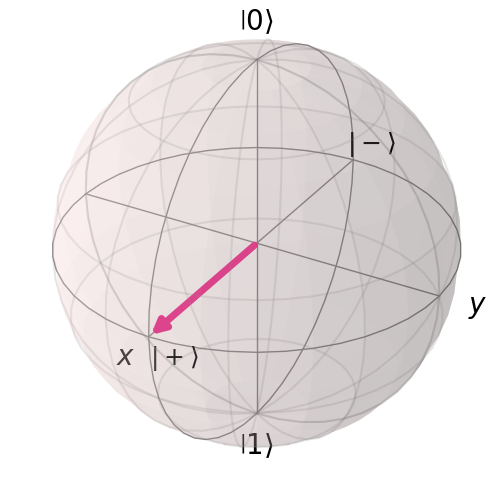
\includegraphics[width=\textwidth]{img/Bloch/bloch_state_+.png}
            \caption{Estado $|+\rangle$ en la esfera de Bloch}
        \end{subfigure}
        \hspace{30mm}
        \begin{subfigure}[t]{0.3\textwidth}
            \centering
            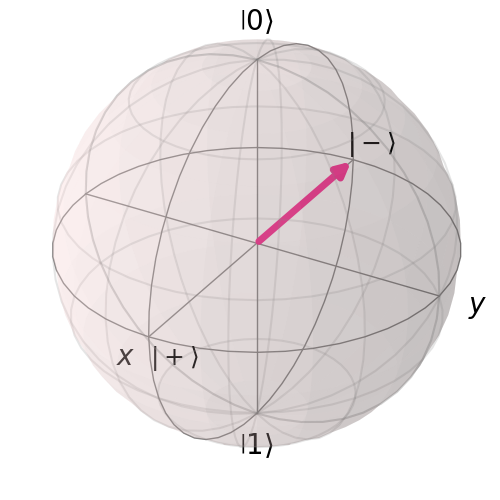
\includegraphics[width=\textwidth]{img/Bloch/bloch_state_-.png}
            \caption{Estado $|-\rangle$ en la esfera de Bloch}
        \end{subfigure}
    \end{figure}

    \vspace{2.5mm}

    Esto lo vimos en (\ref{eq: estados_eje_x_y}) cuando definimos los estados \( \ket{+} \) y \( \ket{-} \), y ahora hemos demostrado de donde salen. Estas son las puertas cuánticas de 1 qubit que principalmente vamos a usar, de manera que si aparece alguna otra puerta simple de 1 qubit la definiremos más adelante conforme nos vayan saliendo. Con esto damos por terminada esta sección y damos paso a la siguiente, en la que discutiremos qué sucede cuando tenemos más de 1 qubit\ldots



    






    \newpage
    \thispagestyle{empty}
    \mbox{}

    \section{Múltiples Qubits}\label{sec: multiples_qubits}

    \vspace{5mm}

    En esta sección, vamos a ver que se siguen las mismas reglas cuando tenemos más de un qubit que a la hora de tener solo uno, como vimos en la sección pasada (\ref{sec: el_qubit}). En este caso ya no estamos hablando de un qubit y por lo tanto, no nos encontramos en un espacio de Hilbert de dos dimensiones, sino que vamos a lograr generalizar las expresiones vistas en la sección anterior (\ref{sec: el_qubit}) para \( N \) qubits, llegando a las mismas expresiones que vimos en el espacio de Hilbert (\ref{sec: el_espacio_de_Hilbert}), y en este caso al tratarse de \( N \) qubits, tendríamos un espacio de Hilbert de \( 2^{N} \) dimensiones.


    \vspace{5mm}

    Para una mejor explicación, vamos a comenzar por un espacio de Hilbert de cuatro dimensiones, es decir, un sistema cuántico de dos qubits. Los estados de este sistema se pueden representar como

    \begin{equation}
        \ket{0 0} = \ket{0} \otimes \ket{0} = \ket{0} \ket{0}
    \end{equation}

    \vspace{2.5mm}

    Entonces, el resto de estados los podemos conseguir de la misma manera que sumamos números binarios, obteniendo que la base \( Z \) está formada por los siguientes estados

    \begin{equation*}
        Z = \{ \ket{0 0}, \ket{0 1}, \ket{1 0}, \ket{1 1} \}
    \end{equation*}

    \vspace{2.5mm}

    De manera que el estado de un qubit de carácter genérico es una superposición de estados en el eje \( Z \)

    \begin{equation}
        \ket{\psi} = c_{0} \ket{0 0} + c_{1} \ket{0 1} + c_{2} \ket{1 0} + c_{3} \ket{1 1}
        \label{eq: superposicion_qubit_2_estados}
    \end{equation}

    \vspace{2.5mm}

    Y las probabilidades de obtener los distintos estados \( \{ \ket{0 0}, \ket{0 1}, \ket{1 0}, \ket{1 1} \} \) al medir sobre el eje \( Z \) son \( | c_{0} |^{2} \), \( | c_{1} |^{2} \), \( | c_{2} |^{2} \) y \( | c_{3} |^{2} \), respectivamente. Hasta aquí no hay nada nuevo, pero ¿Qué sucede cuando queremos dar el paso a \( N \) qubits? Para esto necesitamos pasar los distintos estados de la base \( Z \) de binario a decimal. Suponiendo que los estados del eje \( Z \) se encuentran en la base binaria

    \begin{equation*}
        \ket{b_{N - 1} \ \cdots \ b_{2} \ b_{1} \ b_{0}}, \qquad \forall \ b_{n} \in \{0, 1\}
    \end{equation*}

    \vspace{2.5mm}

    Podemos realizar la conversión a decimal como sigue
    
    \begin{equation}
        \ket{b_{N - 1} \ \cdots \ b_{2} \ b_{1} \ b_{0}} = \ket{ 2^{N - 1} b_{N - 1} + \cdots + 2^{2} b_{2} + 2^{1} b_{1} + 2^{0} b_{0} }
        \label{eq: conversion_qubits_binario_decimal}
    \end{equation}

    \vspace{2.5mm}

    Y esta notación nos permite desarrollar el estado en superposición de un qubit \( \ket{\psi} \) que vimos en (\ref{eq: superposicion_qubit_2_estados}) cuando teníamos dos qubits, pero ahora teniendo \( N \) qubits

    \begin{equation}
        \ket{\psi} = \sum_{j = 0}^{N - 1} c_{j} \ket{j} = c_{0} \ket{0} + c_{1} \ket{1} + c_{2} \ket{2} + \cdots + c_{N - 1} \ket{N - 1}, \qquad j \in \mathbb{N} 
        \label{eq: estado_qubit_dimension_N}
    \end{equation}

    \vspace{2.5mm}

    Esta expresión nos resulta muy familiar, y es que ya la definimos anteriormente en (\ref{eq: combinacion_lineal_Hilbert}) cuando tratábamos los espacios de Hilbert (\ref{sec: el_espacio_de_Hilbert}), por lo que todo encaja muy bien y nos indica que vamos por buen camino. 

    \vspace{5mm}

    A continuación vamos a ver como es la representacón matricial de estos estados, y esto se hace con el denominado \textit{producto de Kronecker}, el cual no vamos a definir formalmente, sino que vamos a ver directamente como funciona, por ejemplo, para el estado \( \ket{0 0} \) en un sistema de dos qubits:

    \begin{equation}
        \ket{0 0} = \ket{0} \ket{0} = \ket{0} \otimes \ket{0} = \begin{pmatrix}
            1 \\
            0
        \end{pmatrix} \otimes \begin{pmatrix}
            1 \\
            0
        \end{pmatrix} = \begin{pmatrix}
            1 \begin{pmatrix} 1 \\ 0 \end{pmatrix} \\
            0 \begin{pmatrix} 1 \\ 0 \end{pmatrix}
        \end{pmatrix} = \begin{pmatrix}
            1 \\
            0 \\
            0 \\
            0
        \end{pmatrix}
        \label{eq: producto_kronecker}
    \end{equation}

    \vspace{2.5mm}

    Si esto lo aplicamos para el resto de estados que definen el eje \( Z \) en un sistema cuántico de dos qubits, obtenemos que

    \begin{equation}
        \ket{0 0} = \begin{pmatrix}
            1 \\
            0 \\
            0 \\
            0 
        \end{pmatrix}, \quad \ket{0 1} = \begin{pmatrix}
            0 \\
            1 \\
            0 \\
            0 
        \end{pmatrix}, \quad \ket{1 0} = \begin{pmatrix}
            0 \\
            0 \\
            1 \\
            0 
        \end{pmatrix}, \quad \ket{1 1} = \begin{pmatrix}
            0 \\
            0 \\
            0 \\
            1 
        \end{pmatrix}
        \label{eq: estados_matricial_2_qubits}
    \end{equation}

    \vspace{2.5mm}

    De manera que podemos expresar el estado de un sistema cuántico de dos qubits mediante un vector columna como vimos en (\ref{eq: vector_sistema_un_qubit}), ampliando la expresión para dos qubits y aplicando lo que acabamos de ver

    \begin{equation}
        \ket{\psi} = c_{0} \ket{0 0} + c_{1} \ket{0 1} + c_{2} \ket{1 0} + c_{3} \ket{1 1} = \begin{pmatrix}
            c_{0} \\
            c_{1} \\
            c_{2} \\
            c_{3}
        \end{pmatrix}
        \label{eq: estado_qubit_dimension_2_matriz}
    \end{equation}

    \vspace{2.5mm}

    Entonces, podemos representar la expresión (\ref{eq: estado_qubit_dimension_N}) como un vector columna de dimension \( N \), siendo \( N \) el número de qubits de nuestro sistema cuántico:

    \begin{equation}
        \ket{\psi} = \sum_{j = 0}^{N - 1} c_{j} \ket{j} = c_{0} \ket{0} + c_{1} \ket{1} + c_{2} \ket{2} + \cdots + c_{N - 1} \ket{N - 1} = \begin{pmatrix}
            c_{0} \\
            c_{1} \\
            c_{2} \\
            \vdots \\
            c_{N - 1}
        \end{pmatrix}
        \label{eq: estados_qubit_dimension_N_matriz}
    \end{equation}

    \vspace{2.5mm}

    Toda esta notación funciona exactamente igual para los bra, como por ejemplo \( \bra{0 0} \):

    \begin{equation*}
        \bra{0 0} = \bra{0} \otimes \bra{0} = \begin{pmatrix}
            1 & 0
        \end{pmatrix} \otimes \begin{pmatrix}
            1 & 0
        \end{pmatrix} = \begin{pmatrix}
            1 \begin{pmatrix} 1 & 0 \end{pmatrix} & 0 \begin{pmatrix} 1 & 0 \end{pmatrix}
        \end{pmatrix} = \begin{pmatrix}
            1 & 0 & 0 & 0
        \end{pmatrix}
    \end{equation*}

    \vspace{2.5mm}

    Entonces, de la misma manera que acabamos de ver en (\ref{eq: estados_qubit_dimension_N_matriz}) un ket generalizado para \( N \) qubits, ahora tenemos un bra generalizado para \( N \) qubits:

    \begin{equation}
        \bra{\psi} = \sum_{j = 0}^{N - 1} c_{j}^{*} \bra{j} = c_{0}^{*} \bra{0} + c_{1}^{*} \bra{1} + c_{2}^{*} \bra{2} + \cdots + c_{N - 1}^{*} \bra{N - 1} = \begin{pmatrix}
            c_{0}^{*} & c_{1}^{*} & c_{2}^{*} & \cdots & c_{N - 1}^{*}
        \end{pmatrix}
        \label{eq: bra_qubit_dimension_N_matriz}
    \end{equation}

    \vspace{10mm}

    


    \subsection{Puertas Cuánticas de Múltiples Qubits}\label{subsection: puertas_cuanticas_multiples_qubits}

    \vspace{5mm}

    De la misma manera que vimos en las puertas cuánticas de un único qubit, las puertas cuánticas aplicadas a más de un qubit siguen siendo transformaciones del estado del qubit \( \ket{\psi} \) en otro \( \ket{\psi'} \), solo que ahora al tener más de una unidad de información cuántica no son rotaciones en la esfera de Bloch, y esto es porque no se pueda representar algo que esté más allá de las tres dimensiones, como vimos anteriormente en los estados de \( Z \) que eran vectores columna de cuatro elementos.

    \vspace{5mm}

    Vamos a comenzar creando algunas puertas de dos qubits. Aunque esto suene tedioso, es algo bastante sencillo si tenemos en cuenta lo que hemos visto anteriormente para puertas de un qubit en (\ref{subsection: puertas_cuanticas_de_1_qubit}), con la idea de que podemos aplicar cualquiera de estas transformaciones a los distintos qubits de \( \ket{\psi} \). Tomemos como ejemplo la puerta de Hadamard \textit{H} y la \textit{NOT} para un qubit, podemos aplicarlas a los distintos qubits de \( \ket{\psi} \), los cuales vamos a suponer que se encuentran en \( \ket{0 0} \)

    \begin{equation*}
        (H \otimes X) \ket{\psi} = (H \otimes X) \ket{0 0} = (H \otimes X) \ket{0} \otimes \ket{0} = H \ket{0} \otimes X \ket{0} = \ket{+} \otimes \ket{1} =
    \end{equation*}
    \begin{equation*}
        = \frac{1}{\sqrt{2}} \left( \ket{0} + \ket{1} \right) \otimes \ket{1} = \frac{1}{\sqrt{2}} \left( \ket{0} \otimes \ket{1} + \ket{1} \otimes \ket{1} \right) = \frac{1}{\sqrt{2}} \left( \ket{0 1} + \ket{1 1} \right)
    \end{equation*}

    \vspace{2.5mm}

    Y de esta manera podemos ver perfectamente que se ha aplicado una puerta \textit{H} al qubit en la izquierda y una puerta \textit{X} al qubit de la derecha. Este resultado también lo podemos obtener matricialmente ya que \( \otimes \) es el producto de Kronecker. Vamos a definir primero la matriz que representa esta puerta cuántica

    \begin{equation*}
        H \otimes X = \frac{1}{\sqrt{2}} \begin{pmatrix}
            1 & 1 \\
            1 & -1 
        \end{pmatrix} \otimes \begin{pmatrix}
            0 & 1 \\
            1 & 0 
        \end{pmatrix} = \frac{1}{\sqrt{2}} \begin{pmatrix}
            1 \begin{pmatrix} 0 & 1 \\ 1 & 0 \end{pmatrix} & 1 \begin{pmatrix} 0 & 1 \\ 1 & 0 \end{pmatrix} \\  
            1 \begin{pmatrix} 0 & 1 \\ 1 & 0 \end{pmatrix} & -1 \begin{pmatrix} 0 & 1 \\ 1 & 0 \end{pmatrix}
        \end{pmatrix} = \frac{1}{\sqrt{2}} \begin{pmatrix}
            0 & 1 & 0 & 1 \\
            1 & 0 & 1 & 0 \\
            0 & 1 & 0 & -1 \\
            1 & 0 & -1 & 0
        \end{pmatrix}
    \end{equation*}

    \vspace{2.5mm}

    Vemos que esta matriz es unitaria, por lo que se verifica que es una puerta cuántica perfectamente válida. Entonces, si multiplicamos esta matriz por el estado \( \ket{0 0} \) de \( \ket{\psi} \) obtenemos, como debería de ser, el mismo resultado

    \begin{equation*}
        \left( H \otimes X \right) \ket{0 0} =  \frac{1}{\sqrt{2}} \begin{pmatrix}
            0 & 1 & 0 & 1 \\
            1 & 0 & 1 & 0 \\
            0 & 1 & 0 & -1 \\
            1 & 0 & -1 & 0
        \end{pmatrix} \begin{pmatrix}
            1 \\
            0 \\
            0 \\
            0
        \end{pmatrix} = \frac{1}{\sqrt{2}} \begin{pmatrix}
            0 \\ 
            1 \\
            0 \\
            1
        \end{pmatrix} = \frac{1}{\sqrt{2}} \left( \ket{0 1} + \ket{1 1} \right)
    \end{equation*}

    \vspace{2.5mm}

    Y así podemos crear nuestras propias puertas cuánticas a nuestro gusto, según nuestras propias necesidades, asegurándonos siempre que sean puertas válidas. Volveremos a este ejemplo más adelante, ya que como veremos, aplicar puertas cuánticas simples de un qubit a un estado con múltiples qubits no puede crear el famoso entrelazamiento cuántico, el cual explicaremos detenidamente en (\ref{sec: entrelazamiento_cuantico}). Sin embargo, podemos tener puertas cuánticas que cambien directamente el estado de dos qubits al mismo tiempo, al contrario de las puertas que hemos visto hasta ahora, y estas son de vital importancia ya que sí permiten crear entrelazamiento. 

    \vspace{5mm}





    \subsubsection{La Puerta CNOT}\label{subsubsection: la_puerta_cnot}

    \vspace{5mm}

    Vamos a ver únicamente dos ejemplos de puertas cuánticas que actúan directamente sobre más de un qubit ya que estas son las más importantes. No obstante, de la misma manera que para las puertas de un único qubit, si en algún otro momento necesitamos definir más puertas cuánticas con algún fin, las definiremos sin problema. Dicho esto, la primera puerta es la famosa \textit{CNOT} (o \textit{controlled-NOT}), la cual actúa sobre un estado de dos qubits como sigue

    \begin{align*}
        \textit{CNOT} \ket{0 0} &= \ket{0 0} \\[5pt]
        \textit{CNOT} \ket{0 1} &= \ket{0 1} \\[5pt]
        \textit{CNOT} \ket{1 0} &= \ket{1 1} \\[5pt]
        \textit{CNOT} \ket{1 1} &= \ket{1 0}
    \end{align*}

    \vspace{2.5mm}

    Podemos ver que en efecto esta puerta es una puerta \textit{NOT} con un qubit de control, de ahí su nombre \textit{CNOT}. Por defecto el qubit de control es el izquierdo, de manera que si dicho qubit es \( \ket{0} \), el estado permanece igual tras aplicar la puerta. Sin embargo si el qubit de control es \( \ket{1} \), se aplica una puerta \textit{NOT} sobre el qubit derecho, de manera que se invierte el estado del qubit. La representación matricial de esta puerta es muy sencilla, ya que al aplicar esta puerta a los estados \( \ket{0 0} \) y \( \ket{0 1} \) estos permanecen igual, y si la aplicamos sobre \( \ket{1 0} \) obtenemos \(1 1\) y viceversa. Esto se traduce en que la última y penúltima columna de la matriz identidad \( I \) están cambiadas, obteniendo la matriz de la puerta \textit{CNOT}
    
    \begin{equation}
        \textit{CNOT} = \begin{pmatrix}
            1 & 0 & 0 & 0 \\
            0 & 1 & 0 & 0 \\
            0 & 0 & 0 & 1 \\
            0 & 0 & 1 & 0
        \end{pmatrix}
        \label{eq: cnot_matriz}
    \end{equation}

    \vspace{2.5mm}

    Y esta puerta tiene su representación en un circuito cuántico, la cual es la siguiente

    \vspace{5mm}

    \begin{figure}[!h]
        \centering
        \scalebox{1.0}{
            $\Qcircuit @C=1.0em @R=0.8em @!R {
                \lstick{\ket{0}} & \targ & \qw & {|1\rangle} \\
                \lstick{\ket{1}} & \ctrl{-1} & \qw & {|1\rangle}
            }$
        }
        \caption{Puerta \textit{CNOT} en un circuito cuántico}
        \label{fig:puerta_cnot_circuito_cuantico}
    \end{figure}
    
    

    \vspace{2.5mm}

    De manera que hemos indicado \( q_{1} \) como el qubit de control y \( q_{0} \) como el resultado de aplicar la puerta \textit{NOT} en los casos que corresponda. También puede darse un segundo caso cuando ambos qubits están intercambiados, por lo que \( q_{0} \) sería el qubit de control en este caso. Esto en un circuito cuántico no tiene mayor complejidad que intercambiar \( q_{0} \) con \( q_{1} \)

    \vspace{5mm}

    \begin{figure}[H]
        \centering
        \scalebox{1.0}{
            $\Qcircuit @C=1.0em @R=0.8em @!R {
                \lstick{\ket{0}} & \ctrl{1} & \qw & {|0\rangle} \\
                \lstick{\ket{1}} & \targ & \qw & {|1\rangle}
            }$
        }        
        \caption{Puerta \(\textit{CNOT}_{01} \) en un circuito cuántico}
        \label{fig: puerta_cnot_01_circuito_cuantico}
    \end{figure}

    \vspace{2.5mm}

    Y esto se denota como \(\textit{CNOT}_{01} \), cuya representación matricial lógicamente cambia:

    \begin{equation}
        \textit{CNOT}_{01} = \begin{pmatrix}
            1 & 0 & 0 & 0 \\
            0 & 0 & 0 & 1 \\
            0 & 0 & 1 & 0 \\
            0 & 1 & 0 & 0
        \end{pmatrix}
    \end{equation}

    \vspace{2.5mm}

    Actuando sobre los estados de dos qubits como sigue

    \begin{align*}
        \textit{CNOT}_{01} \ket{0 0} &= \ket{0 0} \\[5pt]
        \textit{CNOT}_{01} \ket{0 1} &= \ket{1 1} \\[5pt]
        \textit{CNOT}_{01} \ket{1 0} &= \ket{1 0} \\[5pt]
        \textit{CNOT}_{01} \ket{1 1} &= \ket{0 1}
    \end{align*}

    \vspace{2.5mm}

    Esta es una de las puertas más importantes que vamos a ver ya que permite entrelazar dos qubits. De momento, vamos a definir informalmente el entrelazamiento como una conexión que se establece entre ambos, de manera que si el estado de uno de los qubits cambia, también se verá afectado el estado del otro qubit entrelazado. Esto se traduce como que el estado de ambos qubits dependen el uno con el otro, y será el principio fundamental para enviar información cuántica. Todo esto ya lo veremos mucho más detenidamente en (\ref{sec: entrelazamiento_cuantico}), pero ahora vamos a continuar con la segunda puerta cuántica de múltiples qubits que vamos a ver.

    \vspace{5mm}





    \subsubsection{La Puerta de Toffoli}\label{subsubsection: la_puerta_de_toffoli}

    \vspace{5mm}

    Esta puerta es muy similar a la \textit{CNOT} que acabamos de ver, con la diferencia de que esta puerta actúa sobre tres qubits, siendo dos qubits de control. Esto quiere decir que solo se aplica una puerta \textit{NOT} sobre el qubit que no es de control en el caso que estos sean ambos \( \ket{1} \), lo que se suele definir como:

    \begin{equation*}
        \text{Toffoli} \ket{a} \ket{b} \ket{c} = \ket{a} \ket{b} \ket{a b \oplus c}
    \end{equation*}

    \vspace{2.5mm}

    Al actuar sobre tres qubits, la matriz que representa esta puerta es una matriz cuadrada de dimensión \( 2^{3} \), lo que resulta en una matriz con ocho filas y columnas:

    \begin{equation}
        \text{Toffoli} = \begin{pmatrix}
            1 & 0 & 0 & 0 & 0 & 0 & 0 & 0 \\
            0 & 1 & 0 & 0 & 0 & 0 & 0 & 0 \\
            0 & 0 & 1 & 0 & 0 & 0 & 0 & 0 \\
            0 & 0 & 0 & 1 & 0 & 0 & 0 & 0 \\
            0 & 0 & 0 & 0 & 1 & 0 & 0 & 0 \\
            0 & 0 & 0 & 0 & 0 & 1 & 0 & 0 \\
            0 & 0 & 0 & 0 & 0 & 0 & 0 & 1 \\
            0 & 0 & 0 & 0 & 0 & 0 & 1 & 0 
        \end{pmatrix}
        \label{eq: toffoli_matriz}
    \end{equation}

    \vspace{2.5mm}

    Que se puede comprobar que cumple con las condiciones para ser una puerta cuántica, como vimos en (\ref{subsection: puertas_cuanticas_de_1_qubit}). En un circuito cuántico esto se representa simplemente añadiendo un tercer qubit de control a una puerta \textit{CNOT}

    \vspace{2.5mm}

    \begin{figure}[!h]
        \centering
        \scalebox{1.0}{
            $\Qcircuit @C=1.0em @R=0.8em @!R {
                \lstick{\ket{0}} & \ctrl{2} & \rstick{\ket{0}} \qw \\
                \lstick{\ket{1}} & \ctrl{1} & \rstick{\ket{1}} \qw \\
                \lstick{\ket{1}} & \targ    & \rstick{\ket{1}} \qw
            }$
        }
        \caption{Caso de ejemplo de la puerta de Toffoli}\label{fig: puerta_toffoli_circuito_clasico}
    \end{figure}

    Este resultado lo verificar operando directamente con matrices como sigue

    \begin{equation*}
        \text{Toffoli} \ket{0 1 1} = \begin{pmatrix}
            1 & 0 & 0 & 0 & 0 & 0 & 0 & 0 \\
            0 & 1 & 0 & 0 & 0 & 0 & 0 & 0 \\
            0 & 0 & 1 & 0 & 0 & 0 & 0 & 0 \\
            0 & 0 & 0 & 1 & 0 & 0 & 0 & 0 \\
            0 & 0 & 0 & 0 & 1 & 0 & 0 & 0 \\
            0 & 0 & 0 & 0 & 0 & 1 & 0 & 0 \\
            0 & 0 & 0 & 0 & 0 & 0 & 0 & 1 \\
            0 & 0 & 0 & 0 & 0 & 0 & 1 & 0 
        \end{pmatrix} \begin{pmatrix}
            0 \\
            0 \\
            0 \\
            1 \\
            0 \\
            0 \\
            0 \\
            0
        \end{pmatrix} = \begin{pmatrix}
            0 \\
            0 \\
            0 \\
            1 \\
            0 \\
            0 \\
            0 \\
            0
        \end{pmatrix} = \ket{0 1 1}
    \end{equation*}

    \vspace{2.5mm}

    Y vemos que se corresponde a lo previamente explicado. Sin embargo, esto no es todo. Dependiendo del resultado que queramos obtener, vamos a establecer el qubit objetivo (aquel que no es de control) como \( \ket{0} \) o \( \ket{1} \) según la operación que corresponda. Esto es debido a que en la puerta de Toffoli se encuentran intrínsecas muchas de las operaciones que utilizan los ordenadores convencionales, por no decir todas y cada una de ellas.
    
    \vspace{5mm}

    Para ver esto mejor, vamos a definir los qubits de control como \( A \) y \( B \) para introducir un caso genérico, y vamos a analizar el comportamiento de esta puerta, que depende del qubit objetivo, que puede ser \( \ket{0} \) o \( \ket{1} \) como hemos mencionado anteriormente

    \vspace{2.5mm}
    
    \begin{figure}[H]
        \centering
        \begin{subfigure}[t]{0.45\textwidth}
            \centering
            \scalebox{1.0}{
                $\Qcircuit @C=1em @R=0.8em @!R {
                    \lstick{\ket{A}} & \ctrl{2} & \rstick{\ket{A}} \qw \\
                    \lstick{\ket{B}} & \ctrl{1} & \rstick{\ket{B}} \qw \\
                    \lstick{\ket{0}} & \targ    & \rstick{\ket{A B}} \qw
                }$
            }
            \caption{Puerta AND cuántica}\label{fig: puerta_and_cuantica}
        \end{subfigure}
        \hfill
        \begin{subfigure}[t]{0.45\textwidth}
            \centering
            \scalebox{1.0}{
                $\Qcircuit @C=1em @R=0.8em @!R {
                    \lstick{\ket{A}} & \ctrl{2} & \rstick{\ket{A}} \qw \\
                    \lstick{\ket{B}} & \ctrl{1} & \rstick{\ket{B}} \qw \\
                    \lstick{\ket{1}} & \targ    & \rstick{\ket{\overline{A B}}} \qw
                }$
            }
            \caption{Puerta NAND cuántica}\label{fig: puerta_nand_cuantica}
        \end{subfigure}
        \caption{Puerta de Toffoli}\label{fig: puerta_toffoli}
    \end{figure}

    Estas son, en efecto, las puertas \textit{AND} y \textit{NAND} de la computación clásica. Sin quitarle importancia a la puerta \textit{AND}, la puerta \textit{NAND} tiene una pequeña particularidad, y es que con el conjunto de puertas \textit{NAND} podemos obtener todo el resto de puertas lógicas, y por lo tanto, podríamos obtener un ordenador clásico que utilice únicamente esta puerta. Esto se conoce como un conjunto universal de puertas lógicas, ya que a partir de este conjunto (aunque sea una sola puerta) podemos obtener las demás. 
    
    \vspace{5mm}
    
    Vamos a ver que esto es realmente así con algunos ejemplos. En la práctica, para que un conjunto sea universal, tenemos que ser capaces de expresar cada puerta lógica (\textit{AND}, \textit{NOT}, \textit{XOR}) mediante puertas que estén dentro del conjunto universal. Para esto vamos a apoyarnos en el \textit{Álgebra de Boole}, el cual nos va a ayudar a explicar el funcionamiento de las puertas lógicas a través de operaciones booleanas. Comencemos por la puerta \textit{NOT}, la cual se representa como \( \overline{\textit{A}} \)

    \begin{equation*}
        \overline{A} = \overline{A A}
    \end{equation*}

    \vspace{2.5mm}

    Este resultado es muy intuitivo ya que si tenemos un bit \( A \), el cual puede ser \( 0 \) o \( 1 \), el resultado de multiplicar \( A \) consigo mismo, es decir, aplicar una puerta \textit{AND}, siempre va a ser igual a \( A \) ya que \( A = AA \). El segundo caso va ser la puerta \textit{AND}, la cual podemos expresar en términos de varias \textit{NAND} como sigue

    \begin{equation*}
        A B = \overline{ \overline{A B} \cdot \overline{A B} }
    \end{equation*}

    \vspace{2.5mm}

    Este caso puede parecer menos intuitivo que el anterior, pero sigue siendo muy sencillo. Si aplicamos dos puertas \textit{NOT} sobre un bit \( A \) obtenemos el mismo bit, \( A = \overline{\overline{A}}\), entonces, aplicando también el principio anterior obtenemos que \( \overline{ \overline{A B} \cdot \overline{A B} } = \overline{\overline{A B}} = AB \), como queríamos demostrar. El último caso que vamos a ver va a ser la puerta \textit{OR} de la computación clásica

    \begin{equation*}
        A + B =  \overline{ \overline{A A} \ \cdot \ \overline{B B} }
    \end{equation*}

    \vspace{2.5mm}

    La cual vemos que también está compuesta por varias puertas \textit{NAND}. Esto lo hemos logrado aplicando la primera demostración, \( \overline{A} = \overline{A A} \), y posteriormente una de las famosas \textit{Leyes de De Morgan}, la cual establece que \( A + B = \overline{\overline{A} \cdot \overline{B}} \). Estos son únicamente algunos de los ejemplos que se han decidido incluir para darnos cuenta que podemos expresar cualquier puerta clásica a partir de puertas de Toffoli, las cuales son la contrapartida cuántica de la puerta \textit{NAND} que forma un conjunto universal, verificando así que toda información clásica puede ser también descrita mediante un ordenador cuántico.

    \vspace{5mm}

    Sin embargo, no vamos a utilizar únicamente puertas de Toffoli para describir información clásica. Esto lo hemos hecho para demostrar la hipótesis anterior, pero en la realidad no se usan únicamente puertas de Toffoli, ya que nos interesa tener el mínimo de puertas lógicas en un algoritmo o proceso cuántico, para reducir su complejidad al mínimo y mejorar al máximo su rendimiento. Tomando como ejemplo uno de los vistos anteriormente, podemos expresar una puerta \textit{AND} clásica utilizando tres puertas de Toffoli con el qubit objetivo en \( \ket{1} \). Sin embargo, nos interesa mucho más expresar dicha puerta mediante una única puerta de Toffoli, esta vez con el qubit objetivo en \( \ket{0} \), de manera que hemos utilizado una única puerta cuántica en lugar de tres, minimizando el número de puertas como acabamos de explicar.

    \vspace{5mm}

    Con esto damos paso a la siguiente sección, en la que trataremos el entrelazamiento cuántico, el cual es uno de los pilares fundamentales de la computación cuántica y puede crearse a partir de puertas cuánticas que actuán sobre múltiples qubits a la vez, como la \textit{CNOT} vista anteriormente en (\ref{subsubsection: la_puerta_cnot}).

        
        
    
        






    \newpage
    \thispagestyle{empty}
    \mbox{}

    \section{Entrelazamiento Cuántico}\label{sec: entrelazamiento_cuantico}

    \vspace{5mm}
    En esta sección vamos a introducirnos mucho más detalladamente en el \textit{entrelazamiento cuántico}, el cual es uno de los fenómenos más importantes de esta revolución cuántica. Ya dimos al definir la puerta \textit{CNOT} en (\ref{subsubsection: la_puerta_cnot}) una definición muy informal de entrelazamiento cuántico, en la que decíamos que si tenemos dos qubits entrelazados entre sí, un cambio en el estado de uno de ellos afectaba al otro y viceversa. Esto es una propiedad muy potente, ya que nos permite enviar información cuántica, lo cual veremos al final de este capítulo, o en el ámbito de la criptografía generar claves que sean indescifrables, además de otras muchas explotaciones que podemos conseguir con este fenómeno. Para entender mucho mejor esto, vamos a partir de un estado de dos qubits como ya vimos en (\ref{eq: superposicion_qubit_2_estados})

    \begin{equation*}
        \ket{\psi} = c_{0} \ket{0 0} + c_{1} \ket{0 1} + c_{2} \ket{1 0} + c_{3} \ket{1 1}
    \end{equation*}

    \vspace{2.5mm}

    Ya vimos que la probabilidad de obtener \( \ket{0 0} \) en la medición de \( \ket{\psi} \) es \( | c_{0} |^{2} \), midiendo \( \ket{0 1} \) sería \( | c_{1} |^{2} \), y así sucesivamente, siendo la suma del módulo cuadrado de estos coeficientes igual a la unidad. Ahora viene lo nuevo, y es que podemos medir uno de los qubits de \( \ket{\psi} \) individualmente. Si medimos por ejemplo el qubit izquierdo, obtendremos los estados \( \ket{0} \) o \( \ket{1} \) con una cierta probabilidad, las cuales son, en el caso de obtener \( \ket{0} \) 

    \begin{equation*}
        | c_{0} |^{2} + | c_{1} |^{2}
    \end{equation*}

    \vspace{2.5mm}

    En definitiva, la probabilidad de obtener \( \ket{0} \) es igual a la suma del módulo cuadrado de los coeficientes que tienen el qubit que estamos midiendo en \( \ket{0} \). Esto se aplica de la misma manera si medimos \( \ket{1} \), siendo la probabilidad de

    \begin{equation*}
        | c_{2} |^{2} + | c_{3} |^{2}
    \end{equation*}

    \vspace{2.5mm}

    Pero ahora nos puede surgir una duda, ¿A qué estado colapsa \( \ket{\psi} \)? Simplemente colapsa a la superposición de estados cuyo qubit izquierdo es \( \ket{0} \). En nuestro caso, si al medir el qubit de la izquierda este ha colpasado a \( \ket{0} \), nos quedamos con los estados cuyo qubit izquierdo es \( \ket{0} \) y sus respectivos coeficientes, por lo que obtendríamos
    
    \begin{equation*}
        \ket{\psi} = A \left( c_{0} \ket{0 0} + c_{1} \ket{0 1} \right)
    \end{equation*}

    \vspace{2.5mm}

    Siendo \textit{A} una constante de normalización, para que el producto escalar de \( \ket{\psi} \) consigo mismo sea la unidad \( \braket{\psi \ | \ \psi} = 1 \), como debería de ser. Esto aplica de igual manera en el caso de obtener \( \ket{1} \) como resultado de la medición, colapsando \( \ket{\psi} \) en 

    \begin{equation*}
        \ket{\psi} = B \left( c_{2} \ket{1 0} + c_{3} \ket{1 1} \right)
    \end{equation*}

    \vspace{2.5mm}

    Calculando estas constantes, obtenemos ambos estados normalizados

    \begin{equation}
        \frac{c_{0} \ket{0 0} + c_{1} \ket{0 1}}{\sqrt{| c_{0} |^{2} + | c_{1} |^{2}}}, \qquad \frac{c_{2} \ket{1 0} + c_{3} \ket{1 1}}{\sqrt{| c_{2} |^{2} + | c_{3} |^{2}}}
        \label{eq: estados_normalizados}
    \end{equation}

    \vspace{2.5mm}

    Pero, ¿Qué ocurre si vamos un paso más allá? Efectivamente, ahora vamos a medir el qubit derecho, partiendo de uno de los estados que acabamos de ver en (\ref{eq: estados_normalizados}), demostrando así que podemos medir los qubits secuencialmente, uno después del otro, y esto se puede aplicar para un sistema de \textit{N} qubits, pero de momento vamos a seguir con nuestro ejemplo de dos qubits para simplificar cálculos.

    \vspace{5mm}

    Vamos a demostrar que si ahora medimos \( \ket{\psi} \), obtenemos las mismas probabilidades de colapsar en \( \ket{0 0} \), \( \ket{0 1} \), \( \ket{1 0} \) o \( \ket{1 1} \). Hemos de tener en cuenta para este cálculo que primero hemos obtenido un estado con una cierta probabilidad, por lo que la probabilidad total será el producto de la probabilidad de haber obtenido la primera medición por la segunda, quedando

    \begin{align*}
        \ket{0 0} &\rightarrow \left(| c_{0} |^{2} + | c_{1} |^{2}\right) \frac{| c_{0} |^{2}}{\left( \sqrt{| c_{0} |^{2} + | c_{1} |^{2}} \right)^{2}} = | c_{0} |^{2} \\[5pt]
        \ket{0 1} &\rightarrow \left(| c_{0} |^{2} + | c_{1} |^{2}\right) \frac{| c_{1} |^{2}}{\left( \sqrt{| c_{0} |^{2} + | c_{1} |^{2}} \right)^{2}} = | c_{1} |^{2} \\[5pt]
        \ket{1 0} &\rightarrow \left(| c_{2} |^{2} + | c_{3} |^{2}\right) \frac{| c_{2} |^{2}}{\left( \sqrt{| c_{2} |^{2} + | c_{3} |^{2}} \right)^{2}} = | c_{2} |^{2} \\[5pt]
        \ket{1 1} &\rightarrow \left(| c_{2} |^{2} + | c_{3} |^{2}\right) \frac{| c_{3} |^{2}}{\left( \sqrt{| c_{2} |^{2} + | c_{3} |^{2}} \right)^{2}} = | c_{3} |^{2} \\[5pt]
    \end{align*}

    \vspace{2.5mm}

    Y vemos que en efecto estas son las probabilidades iniciales, por lo que acabamos de demostrar que medir el estado de una partícula \( \ket{\psi} \) es lo mismo que medir cada uno de sus qubits secuencialmente, o al menos eso es lo que parece. Esto generalmente es cierto para cualquier \( \ket{\psi} \) siempre y cuando sus qubits no estén entrelazados, ya que si realmente lo están, esto cambia completamente. Supongamos el siguiente estado

    \begin{equation*}
        \ket{\Phi^{+}} = \frac{1}{\sqrt{2}} \left( \ket{0 0} + \ket{1 1} \right)
    \end{equation*}

    \vspace{2.5mm}

    La probabilidad de obtener \( \ket{0} \) o \( \ket{1} \) en la medición del primer qubit es de \( \frac{1}{2} \), siendo la misma probabilidad para ambos estados. Siguiendo (\ref{eq: estados_normalizados}), si obtenemos \( \ket{0} \), el estado \( \ket{\psi} \) colapsa a 

    \begin{equation*}
        \ket{\psi} = A \left( \frac{1}{\sqrt{2}} \ket{0 0} \right)
    \end{equation*}

    \vspace{2.5mm}

    De donde sabemos que la constante de normalización \textit{A} es

    \begin{equation*}
        A = \frac{1}{\sqrt{| c_{0} |^{2}}} = \frac{1}{c_{0}} = \sqrt{2}
    \end{equation*}

    \vspace{2.5mm}

    Por lo tanto el estado de nuestro sistema es

    \begin{equation*}
        \ket{\psi} = \ket{0 0}
    \end{equation*}

    \vspace{2.5mm}

    Y la segunda medición es trivial, ya que hemos obtenido directamente el estado \( \ket{0 0} \). Aplicando lo mismo pero en este caso suponiendo que hemos obtenido \( \ket{1} \) tras la primera medición, tenemos de manera análoga que

    \begin{equation*}
        \ket{\psi} = \ket{1 1}
    \end{equation*}

    \vspace{2.5mm}

    Y esto es nuestro primer caso de entrelazamiento, ya que hemos medido el estado de uno de los qubits de \( \ket{\Phi^{+}} \), y el resultado de la primera medición afecta directamente a la anterior. En este caso, decimos que \( \ket{\Phi^{+}} \) es un \textit{estado máximo entrelazado}, ya que tras la primera medición obtenemos directamente el resultado final con una probabilidad de 1. Esto no siempre tiene por qué ser así, como veremos más adelante, un estado parcialmente entrelazado es muy parecido a esto que acabamos de ver, simplemente que la probabilidad después de la primera medición no es 1, sino que obtendremos unas probabilidades de medición para distintos estados que, por supuesto, al tratarse de qubits entrelazados, estas probabilidades se encuentran condicionadas por el resultado de la medición anterior.

    \vspace{5mm}




    
    \subsection{Estados de Bell}

    \vspace{5mm}

    Para crear entrelazamiento, necesitamos una puerta cuántica que actúe sobre más de un qubit al mismo tiempo. Esto no es posible con las puertas cuánticas de un único qubit, vistas en (\ref{subsection: puertas_cuanticas_de_1_qubit}), ya que al aplicar estas puertas el qubit se transforma pero de una manera independiente del resto, al contrario de las puertas que actúan sobre múltiples qubits, cuyas transformaciones generan en algunos casos una relación de dependencia entre pares de qubits, lo que conocemos como entrelazamiento.

    \vspace{5mm}

    Un ejemplo que puede crear entrelazamiento y que ya vimos anteriormente es la puerta \textit{CNOT}, y podemos obtener el estado \( \ket{\Phi^{+}} \) que ya demostramos en la sección anterior (\ref{sec: entrelazamiento_cuantico}) que es uno de los cuatro estados máximos entrelazados, aplicando una puerta \textit{CNOT} sobre \( \ket{+} \) y \( \ket{0} \):
    
    \begin{equation*}
        \textit{CNOT} \ket{+} \ket{0} = \textit{CNOT} \frac{1}{\sqrt{2}} \left( \ket{0 0} + \ket{1 0} \right) = \frac{1}{\sqrt{2}} \left( \ket{0 0} + \ket{1 1} \right) = \ket{\Phi^{+}}
    \end{equation*}

    \vspace{2.5mm}

    Esto ocurre para todas las combinaciones entre la base sobre el eje \( \textit{X} = \{ \ket{+}, \ket{-} \} \) y sobre el eje \( \textit{Z} = \{ \ket{0}, \ket{1} \} \), obteniendo los cuatro estados máximos entrelazados, conocidos como \textit{Estados de Bell}:

    \begin{align}
        \textit{CNOT} \ket{+} \ket{0} &= \textit{CNOT} \frac{1}{\sqrt{2}} \left( \ket{0 0} + \ket{1 0} \right) = \frac{1}{\sqrt{2}} \left( \ket{0 0} + \ket{1 1} \right) = \ket{\Phi^{+}}, \\[5pt]
        \textit{CNOT} \ket{-} \ket{0} &= \textit{CNOT} \frac{1}{\sqrt{2}} \left( \ket{0 0} - \ket{1 0} \right) = \frac{1}{\sqrt{2}} \left( \ket{0 0} - \ket{1 1} \right) = \ket{\Phi^{-}}, \\[5pt]
        \textit{CNOT} \ket{+} \ket{1} &= \textit{CNOT} \frac{1}{\sqrt{2}} \left( \ket{0 1} + \ket{1 1} \right) = \frac{1}{\sqrt{2}} \left( \ket{0 1} + \ket{1 0} \right) = \ket{\Psi^{+}}, \\[5pt]
        \textit{CNOT} \ket{-} \ket{1} &= \textit{CNOT} \frac{1}{\sqrt{2}} \left( \ket{0 1} - \ket{1 1} \right) = \frac{1}{\sqrt{2}} \left( \ket{0 1} - \ket{1 0} \right) = \ket{\Psi^{-}}.
        \label{eq: estados_bell}
    \end{align}

    \vspace{2.5mm}

    Y podemos demostrar de manera análoga a la vista para \( \ket{\Phi^{+}} \) que si medimos uno de los dos qubits y secuencialmente medimos el otro, el estado que obtenemos al medir por segunda vez esta directamente relacionado con la medición anterior, confirmando que estos estados son estados máximamente entrelazados. Otra propiedad de un estado entrelazado es que no se pueden expresar como un producto de otros estados. Para ello vamos a tomar como ejemplo el estado de Bell \( \ket{\Phi^{+}} \) y lo vamos a intentar expresar en función del producto de dos estados \( \ket{\psi_{1}} \ket{\psi_{0}} \):

    \begin{equation}
        \ket{\psi_{1}} \ket{\psi_{0}} = \left( \alpha_{1} \ket{0} \beta_{1} \ket{0} \right) \left( \alpha_{1} \ket{0} \beta_{1} \ket{0} \right) = \alpha_{1} \alpha_{0} \ket{0 0} + \alpha_{1} \beta_{0} \ket{0 1} + \beta_{1} \alpha_{0} \ket{1 0} + \beta_{1} \beta_{0} \ket{1 1}
    \end{equation}

    \vspace{2.5mm}

    Y aplicando esto a \( \ket{\Psi^{+}} \) llegamos a 

    \begin{equation*}
        \alpha_{1} \alpha_{0} = \frac{1}{\sqrt{2}}, \quad \alpha_{1} \beta_{0} = 0, \quad \beta_{1} \alpha_{0} = 0, \quad \beta_{1} \beta_{0} = \frac{1}{\sqrt{2}}
    \end{equation*}

    \vspace{2.5mm}

    Y vemos que estas soluciones son muy inconsistentes y se contradicen unas con otras. Esto tambíen nos indica que \( \ket{\Psi^{+}} \) no se puede expresar como un producto de estados \( \ket{\psi_{1}} \ket{\psi_{0}} \) y que por lo tanto, es un estado en entrelazamiento. De manera análoga podemos demostrar que cada uno de los distintos estados de Bell son efectivamente estados entrelazados. A continuación vamos a ver estados que se encuentran parcialmente en entrelazamiento, ya que en esta sección hemos visto únicamente los estados de Bell que son todos estados máximos entrelazados, de esta manera tendremos una visión mucho más clara de como funciona este fenómeno de la computación cuántica y posteriormente veremos algunas de las aplicaciones más importantes que tienen.

    \vspace{5mm}





    \subsubsection{Estados Parcialmente Entrelazados}

    \vspace{5mm}

    Como hemos introducido anteriormente, no todos los estados en entrelazamiento nos garantizan con total certeza el estado de la siguiente medición secuencial como hemos estado viendo hasta ahora con los estados de Bell, existen otros muchos estados en entrelazamiento que se denominan estados parcialmente entrelazados, y esto en definitiva es, que no se garantiza el estado de la siguiente medición secuencial al medir qubits entrelazados. Para ver esto, vamos a considerar el siguiente estado:

    \begin{equation*}
        \ket{\psi} = \frac{\sqrt{3}}{2 \sqrt{2}} \ket{0 0} + \frac{\sqrt{3}}{2 \sqrt{2}} \ket{0 1} + \frac{\sqrt{3}}{4} \ket{1 0} + \frac{1}{4} \ket{1 1} 
    \end{equation*}

    \vspace{2.5mm}

    Si medimos el qubit izquierdo, obtenemos \( \ket{0} \) con una probabilidad de \( \frac{3}{4} \) ya que

    \begin{equation*}
        \left| \frac{\sqrt{3}}{2 \sqrt{2}} \right|^{2} + \left| \frac{\sqrt{3}}{2 \sqrt{2}} \right|^{2} = 2 \ \frac{3}{8} = \frac{3}{4}
    \end{equation*}

    \vspace{2.5mm}

    Y el estado colapsa a 

    \begin{equation*}
        \ket{\psi} = A \left( \frac{\sqrt{3}}{2 \sqrt{2}} \ket{0 0} + \frac{\sqrt{3}}{2 \sqrt{2}} \ket{0 1} \right)
    \end{equation*}

    \vspace{2.5mm}

    Y la constante de normalización \textit{A} la podemos obtener de múltiples maneras. La más intuitiva es sabiendo que la probabilidad total ha de ser igual a 1, obteniendo el valor de \textit{A}

    \begin{equation*}
        \left| A \ \frac{\sqrt{3}}{2 \sqrt{2}} \right|^{2} + \left| A \ \frac{\sqrt{3}}{2 \sqrt{2}} \right|^{2} = 1 \quad \rightarrow \quad A^{2} \ \frac{3}{4} = 1 \quad \rightarrow \quad A = \frac{2}{\sqrt{3}}
    \end{equation*}

    \vspace{2.5mm}

    Y por lo tanto el estado de nuestro qubit colapsa a

    \begin{equation*}
        \ket{\psi} = \frac{1}{\sqrt{2}} \left( \ket{0 0} + \ket{0 1} \right)  
    \end{equation*}

    \vspace{2.5mm}

    Con probabilidades de \( \frac{1}{2} \) de obtener \( \ket{0 0} \) y \( \ket{0 1} \) al medir el segundo qubit. Como podemos observar esto no se trata de un estado máximo entrelazado, ya que la medición del primer qubit no determina instantáneamente el resultado del segundo, sino que obtenemos una probabilidad perfectamente equiparable de \( \frac{1}{2} \), aunque estas probabilidades pueden tener cualquier valor. Para ver esto, vamos a ver el segundo caso, en el que la primera medición da como resultado \( \ket{1} \) con \( \frac{1}{4} \) de probabilidad, colapsando en

    \begin{equation*}
        \ket{\psi} = \frac{\sqrt{3}}{2} \ket{1 0} + \frac{1}{2} \ket{1 1}
    \end{equation*}

    \vspace{2.5mm}

    Cuya constante de normalización ya ha sido calculada de la misma manera que en el caso anterior. Esto nos muestra que la probabilidad de obtener \( \ket{1 0} \) es ahora de \( \frac{3}{4} \) y la de obtener \( \ket{1 1} \) de \( \frac{1}{4} \), probando así que los resultados de las mediciones no son los mismos, ya que estamos ante un caso parcialmente entrelazado, ya que el estado de la segunda medición secuencial de \( \ket{\psi} \) depende del resultado de la primera medición, pero no sabemos el resultado tras la primera medición con total certeza, ya que no estamos ante un caso de entrelazamiento de máximo nivel.

    \vspace{5mm}

    Todo esto nos ayudará a entender mucho mejor las aplicaciones de este fenómeno, como lo es el caso de la teleportación cuántica, en el que nos apoyaremos en los estados de Bell vistos en (\ref{eq: estados_bell}) para enviar información cuántica desde un emisor, el cual recibirá el nombre de Alice, y un receptor, que llamaremos Bob. Todo esto lo vamos a ver a continuación.

    \vspace{5mm}





    \subsection{Teleportación Cuántica}\label{subsection: teleportacion_cuantica}

    \vspace{5mm}

    En esta sección vamos a explicar la teleportación cuántica, el cual es un fenómeno muy importante que surge a partir del entrelazamiento cuántico visto anteriormente en (\ref{sec: entrelazamiento_cuantico}). Este es un proceso en el que utilizaremos bits para enviar información cuántica, y con esto nos referimos al estado de un qubit en superposición \( \ket{\psi} = \alpha \ket{0} + \beta \ket{1} \) de un punto a otro, en el que pondremos nombre propio al emisor, Alice, y también al receptor, comúnmente conocido como Bob.

    \vspace{5mm}

    Llegados a este punto puede surgirnos una duda, ¿Por qué no enviamos la información cuántica directamente desde Alice hasta Bob? De esta manera nos ahorraríamos el uso de bits, sin embargo, esto no es posible, y para explicar esto nos vamos a basar en dos principios básicos que impiden esto, el \textit{Teorema de no-clonación} y la \textit{decoherencia}. Comencemos por el \textit{Teorema de no-clonación}.

    \vspace{5mm}

    \subsubsection{Teorema de No-Clonación}\label{subsubsection: teorema_no_clonacion}

    \vspace{5mm}

    Supongamos que tengamos una partícula \( \ket{\psi} \) cuyo estado es conocido, como por ejemplo \( \ket{+} \). Esto nos permite clonar el estado de \( \ket{\psi} \) simplemente aplicando una puerta de Hadamard sobre \( \ket{0} \), creando tantas copias de \( \ket{\psi} \) como queramos:

    \begin{equation*}
        \ket{+} \ket{0} \ \overset{I \otimes H}{\longrightarrow} \ \ket{+} \ket{+}
    \end{equation*}

    \vspace{2.5mm}

    De manera que clonar el estado de un qubit conocido no es problema, el problema viene cuando no es conocido, como en el caso que acabamos de ver de enviar el estado de un qubit en superposición de Alice a Bob

    \begin{equation}
        \ket{\psi} = \alpha \ket{0} + \beta \ket{1}
    \end{equation}

    \vspace{2.5mm}

    Para conseguir duplicar el estado de \( \ket{\psi} \) necesitamos una puerta cuántica que satisfaga

    \begin{equation*}
        \ket{\psi} \ket{0} \ \overset{U}{\longrightarrow} \ \ket{\psi} \ket{\psi}
    \end{equation*}

    \vspace{2.5mm}

    Esta puerta cuántica la vamos a denotar como \textit{U}, de unitario, una de las propiedades que han de cumplir estas puertas y que ya vimos en (\ref{eq: puertas_cuanticas_unitarias}). Entonces, se ha de satisfacer lo siguiente:
    
    \begin{equation*}
        U \ket{\psi} \ket{0} = \ket{\psi} \ket{\psi}
    \end{equation*}

    \vspace{2.5mm}

    Y apoyándonos en el álgebra lineal, podemos obtener un sistema de ecuaciones que satisfaga la condición anterior:

    \begin{gather*}
        \begin{pmatrix}
            U_{11} & U_{12} & U_{13} & U_{14} \\
            U_{21} & U_{22} & U_{23} & U_{24} \\
            U_{31} & U_{32} & U_{33} & U_{34} \\
            U_{41} & U_{42} & U_{43} & U_{44}
        \end{pmatrix} \begin{pmatrix}
            \alpha \\
            \beta
        \end{pmatrix} \otimes \begin{pmatrix}
            1 \\
            0
        \end{pmatrix} = \begin{pmatrix}
            \alpha \\
            \beta
        \end{pmatrix} \otimes \begin{pmatrix}
            \alpha \\
            \beta
        \end{pmatrix} \\[5pt]
        \begin{pmatrix}
            U_{11} & U_{12} & U_{13} & U_{14} \\
            U_{21} & U_{22} & U_{23} & U_{24} \\
            U_{31} & U_{32} & U_{33} & U_{34} \\
            U_{41} & U_{42} & U_{43} & U_{44}
        \end{pmatrix} \begin{pmatrix}
            \alpha \\
            0 \\
            \beta
            0 \\
        \end{pmatrix} = \begin{pmatrix}
            \alpha^{2} \\
            \alpha \beta \\
            \alpha \beta \\
            \beta^{2}
        \end{pmatrix} \\[5pt]
        \begin{pmatrix}
            U_{11} \alpha + U_{13} \beta \\
            U_{21} \alpha + U_{23} \beta \\
            U_{31} \alpha + U_{33} \beta \\
            U_{41} \alpha + U_{43} \beta 
        \end{pmatrix} = \begin{pmatrix}
            \alpha^{2} \\
            \alpha \beta \\
            \alpha \beta \\
            \beta^{2}
        \end{pmatrix}
    \end{gather*}

    \vspace{2.5mm}

    Y con esto podemos ver perfectamente que las soluciones de este sistema dependen de \( \alpha \) y \( \beta \), por lo que acabamos de demostrar que no podemos clonar ningún estado desconocido, ya que para ello necesitamos saber el valor de \( \alpha \) y de \( \beta \).

    \vspace{5mm}

    \subsubsection{Decoherencia}

    \vspace{5mm}

    El otro fenómeno que hace imposible duplicar el estado de \( \ket{\psi} \) se conoce como decoherencia. La decoherencia es un fenómeno que sucede cuando un sistema cuántico interactúa con las propiedades del entorno, y como resultado podemos perder información, ya que lo que sucede es que el estado nuestro sistema cuántico \( \ket{\psi} \) se ve alterado, por lo que si tenemos un qubit en \( \ket{0} \), este puede verse ligeramente afectado por la decoherencia, cambiando su valor, como podemos ver en el siguiente ejemplo:

    \vspace{2.5mm}

    \begin{figure}[!h]
        \centering
        \begin{subfigure}[t]{0.45\textwidth}
            \centering
            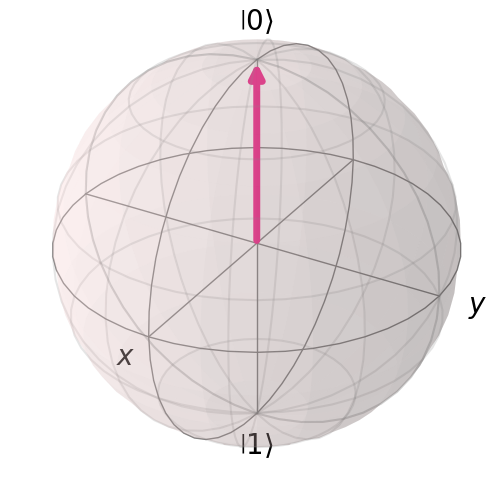
\includegraphics[width=0.70\textwidth]{./img/Bloch/bloch_state_0.png}
            \caption{Estado \( \ket{0} \)}\label{fig: estado_0}
        \end{subfigure}
        \hfill
        \begin{subfigure}[t]{0.45\textwidth}
            \centering
            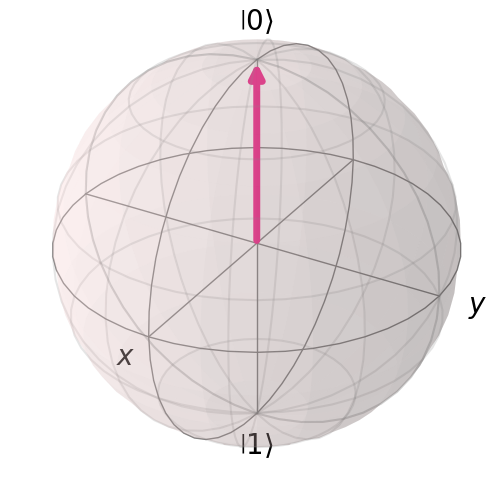
\includegraphics[width=0.70\textwidth]{./img/Bloch/bloch_state_0.png}
            \caption{Estado alterado por la decoherencia}\label{fig: estado_alterado_decoherencia}
        \end{subfigure}
    \end{figure}

    \vspace{2.5mm}

    Y esto puede ocurrir en múltiples escenarios, por ejemplo en casos de ruido térmico, ya que en este suceso las partículas tienen un cierto ruido térmico, siendo esto una de las principales causas de las alteraciones del estado de los qubits (decoherencia). Es por esto que los ordenadores cuánticos actuales se enfrían los máximo posible, hasta temperaturas del cero absoluto para evitar esta decoherencia producida por el ruido térmico. Otros hechos que pueden provocar decoherencia son la interferencia electromagnética, producida por ejemplo por ondas de microondas, o simplemente defectos en la fabricación de un ordenador cuántico. 

    \vspace{5mm}

    Es por esto que los ordenadores cuánticos son realmente especiales y han de ser tratados con mucha delicadeza, y tenemos que mantenerlos alejados de cualquier interacción que puedan tener con su entorno. Incluso la medición de un qubit puede causar decoherencia, lo que nos ha llevado a la necesidad de métodos y sistemas de corrección de errores cuánticos, causados por estos problemas.

    \vspace{5mm}

    \subsubsection{Teleportación Cuántica}

    \vspace{5mm}

    Una vez ya hemos aclarado por qué no podemos enviar información cuántica directamente y la razón por la que tenemos que apoyarnos en información clásica (bits), vamos a entrar de lleno en la teleportación cuántica. Como ya introdujimos anteriormente en (\ref{subsection: teleportacion_cuantica}), vamos enviar el estado de un qubit cuántico \( \ket{\psi} = \alpha \ket{0} + \beta \ket{1} \) de Alice a Bob, apoyándonos en información clásica y en el entrelazamiento, aplicando todas las propiedades que el entrelazamiento tiene sobre \( \ket{\psi} \).

    \vspace{5mm}

    Como no conocemos el estado de \( \ket{\psi} \), Alice no puede duplicarlo sobre un qubit de Bob, como ya vimos en el \textit{Teorema de no-clonación} (\ref{subsubsection: teorema_no_clonacion}), por lo que no podemos comunicarle directamente a Bob el estado de \( \ket{\psi} \). Es este caso uno de los muchos usos del entrelazamiento, en el que le podremos decir a Bob el estado de \( \ket{\psi} \) utilizando únicamente dos bits. Imaginemos que Alice y Bob comparten dos qubits entrelazados en el estado \( \ket{\Phi^{+}} \), de manera que Alice posee dos qubits, \( \ket{\psi} \) el cual es el que queremos transmitir a Bob, y uno de los dos qubits de \( \ket{\Phi^{+}} \), mientras que Bob posee el otro qubit de \( \ket{\Phi^{+}} \), quedando los tres qubits en

    \begin{gather*}
        \ket{\psi} \ket{\Phi^{+}} = \alpha \ket{0} \ket{\Phi^{+}} + \beta \ket{1} \ket{\Phi^{+}} = \alpha \ket{0} \frac{1}{\sqrt{2}} \left( \ket{0 0} + \ket{1 1} \right) + \beta \ket{1} \frac{1}{\sqrt{2}} \left( \ket{0 0} + \ket{1 1} \right) = \\[5pt]
        = \frac{1}{\sqrt{2}} \left[ \alpha \left( \ket{0 0 0} + \ket{0 1 1} \right) + \beta \left( \ket{1 0 0} + \ket{1 1 1} \right)\right]
    \end{gather*}

    \vspace{2.5mm}

    Entonces, el objetivo que tenemos ahora es expresar el estado del qubit de Bob en función de \( \alpha \) y \( \beta \), y debido a que se encuentra entrelazado con uno de los qubits de Alice, Bob va a poder saber el estado de \( \ket{\psi} \) antes de la medición, ya que tendremos que medir el qubit entrelazado de Alice, lo cual afectará directamente al qubit entrelazado de Bob al encontrarse ambos en un estado máximo de entrelazamiento, y Bob podrá conocer de esta manera el estado de \( \ket{\psi} \). Comencemos aplicando una puerta \textit{CNOT} sobre los dos qubits de Alice, los cuales son el qubit izquierdo y el central, obteniendo el siguiente resultado:

    \begin{equation*}
        \frac{1}{\sqrt{2}} \left[ \alpha \left( \ket{0 0 0} + \ket{0 1 1} \right) + \beta \left( \ket{1 0 0} + \ket{1 1 1} \right)\right] \ \overset{\textit{CNOT}}{\longrightarrow} \ \frac{1}{\sqrt{2}} \left[ \alpha \left( \ket{0 0 0} + \ket{0 1 1} \right) + \beta \left( \ket{1 1 0} + \ket{1 0 1} \right)\right]
    \end{equation*}

    \vspace{2.5mm}

    Y a continuación aplicamos una puerta de Hadamard sobre el qubit izquierdo de Alice, y operando obtenemos el siguiente resultado:

    \begin{gather*}
        \frac{1}{\sqrt{2}} \left[ \alpha \left( \ket{0 0 0} + \ket{0 1 1} \right) + \beta \left( \ket{1 1 0} + \ket{1 0 1} \right)\right] \ \overset{H}{\longrightarrow} \ \frac{1}{\sqrt{2}} \left[ \alpha \left( \ket{+ 0 0} + \ket{+ 1 1} \right) + \beta \left( \ket{- 1 0} + \ket{- 0 1} \right)\right] = \\[5pt]
        = \frac{1}{2} \left[ \alpha \left( \ket{0} + \ket{1} \right) \left( \ket{0 0} + \ket{1 1} \right) + \beta \left( \ket{0} - \ket{1} \right) \left( \ket{1 0} + \ket{0 1} \right) \right] = \\[5pt]
        = \frac{1}{2} \left[ \ket{0 0} \left( \alpha \ket{0} + \beta \ket{1} \right) + \ket{0 1} \left( \beta \ket{0} + \alpha \ket{1} \right) + \ket{1 0} \left( \alpha \ket{0} - \beta \ket{1} \right) + \ket{1 1} \left( - \beta \ket{0} + \alpha \ket{1} \right) \right]
    \end{gather*}

    \vspace{2.5mm}

    En esto se resume, a falta del procedimiento a seguir tras la medición, la teleportación cuántica, cuyo circuito viene recogido de la siguiente manera:

    \begin{figure}[h!]
        \centering
        \[
        \Qcircuit @C=1em @R=1.5em {
        & \qw & \qw      & \qw      & \qw       & \qw & \qw & \qw & \gate{X} \cwx & \qw & \gate{Z} \qw & \rstick{|\psi\rangle} \qw \\
                                & \qw & \targ    & \qw & \qw & \qw & \meter  & \cw & \control \cwx \cw & \cw & \cwx \cw & \cw & \\
        \lstick{|\psi\rangle}   & \qw & \ctrl{-1}    & \qw & \gate{H} & \qw & \meter  & \cw & \cw & \cw & \control \cwx \cw & \cw & \\
        \inputgroupv{1}{2}{0.8em}{1.5em}{\ket{\Phi^+}} \ 
        }
        \]
        \caption{Teleportación cuántica. Circuito cuántico}\label{fig: circuito_teleportacion}
        \end{figure}

    \vspace{2.5mm}

    Ahora es cuando viene el momento de la medición. Si Alice mide sus dos qubits, estos colapsarán a uno de los siguientes estados con una probabilidad equiparable de \( \frac{1}{4} \):

    \begin{align}
        \ket{0 0} &\left( \alpha \ket{0} + \beta \ket{1} \right)\label{eq: medicion_1} \\[5pt]
        \ket{0 1} &\left( \beta \ket{0} + \alpha \ket{1} \right)\label{eq: medicion_2} \\[5pt]
        \ket{1 0} &\left( \alpha \ket{0} - \beta \ket{1} \right)\label{eq: medicion_3} \\[5pt]
        \ket{1 1} &\left( - \beta \ket{0} + \alpha \ket{1} \right)\label{eq: medicion_4}
    \end{align}

    \vspace{2.5mm}
    Y aquí ya tenemos los qubits de Alice, los cuales ya vemos que han colapsado a \( \ket{0 0} \), \( \ket{0 1} \), \( \ket{1 0} \) o \( \ket{1 1} \), y tenemos también el qubit de Bob expresado en función de \( \alpha \) y \( \beta \), de manera que Alice solo tiene que comunicarle a Bob el resultado de la medición de sus dos qubits, y dependiendo del resultado, Bob tendrá que aplicar una determinada puerta cuántica a su qubit, obteniendo finalmente \( \ket{\psi} \):

    \begin{itemize}
        \item Si la medición colapsó a \( \ket{0 0} \) (\ref{eq: medicion_1}), Bob ya tiene directamente su qubit en el mismo que estado que \( \ket{\psi} \), por lo que no tendríamos que aplicar ninguna puerta cuántica.
        \item Si tras la medición obtenemos \( \ket{0 1} \) (\ref{eq: medicion_2}), Bob aplicará una puerta \textit{NOT} (o puerta \textit{X}) para obtener \( \ket{\psi} \).
        \item Si obtenemos \( \ket{1 0} \) (\ref{eq: medicion_3}) tras la medición, simplemente Bob aplica una puerta \textit{Z} a su qubit, llegando finalmente a \( \ket{\psi} \).
        \item Y si por último Alice obtiene \( \ket{1 1} \) (\ref{eq: medicion_4}) tras la medición, Bob aplicaría una puerta \textit{X} seguida de una \textit{Z} para obtener \( \ket{\psi} \).
    \end{itemize}

    \vspace{5mm}

    Y esta es la magia de la teleportación cuántica, la cual surge ante el problema de no poder enviar físicamente información cuántica debido a problemas como el teorema de no-clonación o la decoherencia. Es por esto que aprovechamos las propiedades del entrelazamiento cuántico para asentar las bases que nos permiten describir el estado de un qubit de un emisor, en este caso Alice, a un receptor, Bob, tomando de la mano el uso de puertas cuánticas vistas en (\ref{subsection: puertas_cuanticas_multiples_qubits}) como la \textit{CNOT} y la puerta de Hadamard \textit{H}.

    \vspace{5mm}





    \subsection{Encriptación Cuántica. BB84}\label{subsection: bb84}

    \vspace{5mm}

    Digamos ahora que Alice y Bob quieren mandar un mensaje, pero de manera segura, ya que la información enviada entre ambos pueden ser datos confidenciales, contraseñas, etc. Es por esto que ciertas personas nos van a intentar robar esta información, y nos solemos referir a estas personas en el aḿbito de la criptografía cuántica como Eve, y de la misma manera que en la computación clásica se estableceremos una clave pública y privada para que Bob descifre la información enviada por Alice. Es en esto en lo que se basa el protocolo que vamos a ver en este capítulo, BB84.

    \vspace{5mm}

    Aunque es cierto que BB84 no necesita entrelazamiento, nos servirá para asentar las bases de un sistema de encriptación más complejo, como EPR (\ref{subsection: epr}) o E91 (\ref{subsection: e91}), los cuales sí usan entrelazamiento y son protocolos más seguros. Estos son solo algunos ejemplos de QKD (Quantum Key Distribution), métodos o protocolos en el que por medio de una encriptación cuántica aseguramos la la seguridad e integridad de la información transmitida. Comencemos por el primer paso de BB84, en el que el emisor, en este caso Alice, selecciona un conjunto de bits, y para cada bit se escoge aleatoriamente una base, que puede ser la base en el eje \textit{Z} \( \{ \ket{0}, \ket{1} \} \) o en el eje \textit{X} \( \{ \ket{+}, \ket{-} \} \), como se puede ver recogido en la siguiente tabla:

    \vspace{2.5mm}

    \begin{figure}[H]
        \centering
        \renewcommand{\arraystretch}{1.25} 
        \begin{tabular}{|l|ccccccccc|}
            \hline
            Bits de Alice & 1 & 0 & 0 & 1 & 0 & 0 & 0 & 1 & 1 \\
            Bases de Alice & X & Z & Z & X & X & Z & X & Z & Z \\ \hline
        \end{tabular}
        \caption{Primer paso de BB84.}\label{fig: primer_paso_bb84}
    \end{figure}

    \vspace{2.5mm}

    El siguiente paso es muy sencillo, y es que dependiendo del bit inicial y la base escogida, Alice va a enviar un estado u otro. Comenzando por la base \textit{Z}, si el bit inicial es 0, Alice le enviará a Bob el estado \( \ket{0} \), y si inicialmente se escogió 1, se envía \( \ket{1} \). Esto aplica de la misma manera para la base en el eje \textit{X}, en el que enviaremos \( \ket{+} \) o \( \ket{-} \) dependiendo si inicialmente se escogió 0 o 1, respectivamente, como podemos ver en la siguiente tabla:

    \vspace{2.5mm}

    \begin{figure}[H]
        \centering
        \renewcommand{\arraystretch}{1.25} 
        \begin{tabular}{|l|ccccccccc|}
            \hline
            Bits de Alice \ & 1       & 0       & 0       & 1       & 0       & 0       & 0       & 1       & 1 \\
            Base            & X       & Z       & Z       & X       & X       & Z       & X       & Z       & Z \\
            Se envía        & \ket{+} & \ket{0} & \ket{0} & \ket{+} & \ket{-} & \ket{-} & \ket{-} & \ket{1} & \ket{1} \\ \hline
        \end{tabular}
        \caption{Segundo paso de BB84.}\label{fig: segundo_paso_bb84}
    \end{figure}

    \vspace{2.5mm}

    A continuación Bob recibe la información enviada por Alice, y Bob mide el resultado que Alice le acaba de enviar en una de las dos bases que estamos utilizando, \textit{Z} o \textit{X}, de manera que si la base elegida por Bob coincide con la escogida por Alice, el resultado será el mismo que Alice, ya que la información que estamos enviando se encuentra en los polos de los ejes con los que estamos trabajando, por lo que no tenemos ninguna incertidumbre en la medición y sabemos el resultado. Por el contrario, si la base es distinta, tendremos \( \frac{1}{2} \) de probabilidad de acertar el resultado o de errarlo, siendo el resultado de Bob completamente aleatorio ya que la probabilidad es la misma, quedando en

    \vspace{2.5mm}

    \begin{figure}[H]
        \centering
        \renewcommand{\arraystretch}{1.25} 
        \begin{tabular}{|l|ccccccccc|}
            \hline
            Bits de Alice \ & 1       & 0       & 0       & 1       & 0       & 0       & 0       & 1       & 1 \\
            Base            & X       & Z       & Z       & X       & X       & Z       & X       & Z       & Z \\
            Se envía        & \ket{+} & \ket{0} & \ket{0} & \ket{+} & \ket{-} & \ket{-} & \ket{-} & \ket{1} & \ket{1} \\ \hline
            Base de Bob     & Z       & Z       & X       & X       & X       & Z       & Z       & X       & X \\
            Medición        & \ket{0} & \ket{0} & \ket{-} & \ket{+} & \ket{-} & \ket{-} & \ket{1} & \ket{-} & \ket{+} \\
            Bit final       & 0       & 0       & 1       & 0       & 1       & 1       & 1       & 1       & 0 \\ \hline
        \end{tabular}
        \caption{Obtención del bit final BB84.}\label{fig: obtencion_bit_final_bb84}
    \end{figure}

    \vspace{2.5mm}

    En este momento es cuando determinamos la clave privada para comunicarnos con total seguridad, aunque siempre puede existir una pequeña probabilidad de que nos intercepten la clave, por muy pequeña que sea, lo cual veremos muy proximamente. Para establecer la clave, Alice y Bob revelan públicamente las bases que ambos han usado, y si ambas bases coinciden, saben perfectamente que su resultado es el mismo, obteniendo así los bits de la clave privada:

    \vspace{2.5mm}

    \begin{figure}[H]
        \centering
        \renewcommand{\arraystretch}{1.25} 
        \begin{tabular}{|l|ccccccccc|}
            \hline
            Bits de Alice \ & 1       & 0       & 0       & 1       & 0       & 0       & 0       & 1       & 1 \\
            Base            & X       & Z       & Z       & X       & X       & Z       & X       & Z       & Z \\
            Se envía        & \ket{+} & \ket{0} & \ket{0} & \ket{+} & \ket{-} & \ket{-} & \ket{-} & \ket{1} & \ket{1} \\
            Base de Bob     & Z       & Z       & X       & X       & X       & Z       & Z       & X       & X \\
            Medición        & \ket{0} & \ket{0} & \ket{-} & \ket{+} & \ket{-} & \ket{-} & \ket{1} & \ket{-} & \ket{+} \\
            Bit final       & 0       & 0       & 1       & 0       & 1       & 1       & 1       & 1       & 0 \\ \hline
            Clave Privada   &         & 0       &         & 0       & 1       & 1       &         &         & \\ \hline
        \end{tabular}
        \caption{Obtención de la clave privada mediante BB84.}\label{fig: obtencion_clave_privada_bb84}
    \end{figure}

    \vspace{2.5mm}

    Por lo que la clave es 0011. Sin embargo, podemos tener un problema, y es que haya una tercera partida, Eve, que esté intentando robarnos los datos. Supongamos que Alice selecciona la base \textit{Z} y envía \( \ket{0} \) a Bob, pero Eve intercepta el estado \( \ket{0} \). Ahora Eve tiene dos opciones, seleccionar la base \textit{Z} por lo que al medir el resultado seguiría siendo \( \ket{0} \), o el caso contrario, en el que escoja una base distinta de Alice. En este caso, sería la base \textit{X}, por lo que al medir \( \ket{0} \) podría obtener o bien \( \ket{0} \) o \( \ket{1} \), y en caso de medir \( \ket{1} \), Alice y Bob se darían cuenta que hay una tercera persona robando los datos, ya que los casos que nos interesan son en el que las bases de Alice y Bob coinciden, estableciendo así la clave. En definitiva, la probabilidad de detectar a Eve en un único qubit es de \( \frac{1}{4} \), y entonces, la probabilidad de que Eve pase desapercibido es \( \frac{3}{4} \). Esto lo podemos generalizar para \textit{n} bits, siendo la probabilidad de detectar a Eve de

    \begin{equation*}
        \text{Probabilidad de detectar a Eve} = 1 - \left( \frac{3}{4} \right)^{n}
    \end{equation*}

    \vspace{2.5mm}

    Siendo esta probabilidad de 0.99999943 para 50 bits, por lo que la probabilidad de que Eve acceda a la información sin ser detectada es prácticamente nula. No obstante, al medir Eve los qubits enviados de Alice, el estado de estos puede colapasar a un estado que no es el que teníamos previsto, alterando la información. Para solucionar este problema simplemente añadimos unos bits de prueba a nuestra cadena de bits original, y de esta manera primero comprobaríamos si hay algún fallo al obtener la clave de la cadena de bits de prueba, la cual no es una parte de nuestra clave real, es una pequeña comprobación para verificar que todo va en orden.

    

    \vspace{5mm}



    \vspace{5mm}

    \subsection{El Protocolo E91}\label{subsection: e91}

    \vspace{5mm}

    El protocolo BB84 (\ref{subsection: bb84}) es una de las principales bases de la encriptación cuántica, ya que la mayoría de protocolos de este ámbito se basan en él, y el protocolo que vamos a ver a continuación, \textit{E91}, cuyas siglas hacen referencia a su autor, \textit{Artur Ekert} en 1991~\cite{ekert_Original}, no va a ser menos. La principal diferencia es que este sistema sí utiliza qubits entrelazados, añadiendo así una capa de seguridad adicional contra Eve.

    \vspace{5mm}

    Una vez se reparten los pares de qubits entrelazados \( q_{j}, q_{j}' \) entre Alice y Bob, cada uno eligen una base con la que medir sus qubits entrelazados, \( \{ \vec{a_{1}}, \vec{a_{2}}, \vec{a_{3}} \} \) y \( \{ \vec{b_{1}}, \vec{b_{2}}, \vec{b_{3}} \} \) respectivamente, y estas bases tienen que cumplir unas ciertas condiciones que veremos más adelante. Estas bases usadas para medir cada uno de los qubits se mantienen en secreto hasta que se cumple con todas las mediciones. Posteriormente Alice y Bob comparten públicamente las bases que han utilizado para cada qubit, de manera que si estas bases coinciden, el resultado de ambos será el mismo ya que los qubits se encuentran máximamente entrelazados en el estado de Bell \( \ket{\Phi^{+}} \), determinando así la clave privada, y los casos en los que las bases no coincidan, serán reservados para averiguar si la comunicación ha sido interceptada por Eve, o si por el contrario ha habido algún problema de ruido o decoherencia, dificultando así la comunicación.

    \vspace{5mm}

    En primer lugar, supongamos que una tercera persona proporciona a Alice y Bob pares de qubits entrelazados entre sí, enviando uno de los qubits entrelazados a Alice y el otro a Bob, los cuales se encuentran en uno de los estados de Bell \( \ket{\Phi^{+}} \):

    \begin{equation*}
        \ket{\Phi^{+}} = \frac{1}{\sqrt{2}} \left( \ket{0 0} + \ket{1 1} \right)
    \end{equation*}

    \vspace{2.5mm}

    Una vez han recibido correctamente cada uno de sus qubits entrelazados y están listos para la comunicación, ambos eligen una base entre las dos posibles opciones con la que medir el qubit. Las bases que vamos a usar las vamos a denotar como \( \{ \vec{a_{1}}, \vec{a_{2}}, \vec{a_{3}} \} \) para Alice y \( \{ \vec{b_{1}}, \vec{b_{2}}, \vec{b_{3}} \} \) en el caso de Bob, para hacer un postprocesamiento de los resultados obtenidos con el fin de detectar a Eve o un excesivo ruido cuántico. En definitiva, estas bases son

    \begin{minipage}[t]{0.45\textwidth}
        \begin{align*}
            \vec{a_{1}} &= Z, \\[5pt]
            \vec{a_{2}} &= \frac{1}{\sqrt{2}} \left( X + Z \right), \\[5pt]
            \vec{a_{3}} &= X,
        \end{align*}
    \end{minipage}
    \hspace{0mm}
    \begin{minipage}[t]{0.45\textwidth}
        \begin{align*}
            \vec{b_{1}} &= \frac{1}{\sqrt{2}} \left( X + Z \right) \\[5pt]
            \vec{b_{2}} &= X \\[5pt]
            \vec{b_{3}} &= \frac{1}{\sqrt{2}} \left( X - Z \right)
        \end{align*}
    \end{minipage}

    \vspace{2.5mm}

    Esto lo podemos ver gráficamente con los siguientes ángulos en el plano \textit{XZ}:

    \begin{figure}[H]
        \hspace{7,5mm}
        \begin{subfigure}[t]{0.40\textwidth}
            \centering
            \begin{tikzpicture}[>=Stealth, scale=2.5]
                % z
                \draw[black] (0, -1) -- (0, 1) node[above] {z};
                % x
                \draw[black] (-1, 0) -- (1, 0) node[right] {x};
                % Base a1
                \draw[->, thick, blue] (0, -1) -- (0, 1) node[below left] {$\vec{a_{1}}$};
                \draw[->, thick, blue] (0, 1) -- (0, -1);
                % Base a2 a 45 grados
                \draw[->, thick, red] (0,0) -- (cos{45},sin{45}) node[above right] {$\vec{a_{2}}$}; % 45 degrees
                \draw[->, thick, red] (0,0) -- (cos{225},sin{225}); % Vector opuesto a a2        
                % Base a3
                \draw[->, thick, orange] (-1 ,0) -- (1 ,0) node[below left] {$\vec{a_{3}}$};
                \draw[->, thick, orange] (1 ,0) -- (-1 ,0);
                % Círculo de radio 1
                \draw[dashed] (0,0) circle (1cm);
                % Angulos
                \draw (0.5,0) arc (0:45:0.5);
                \node at (22.5:0.7) {$\frac{\pi}{4}$};       
                \draw (0.5,0) arc (0:90:0.5);
                \node at (67.5:0.7) {$\frac{\pi}{4}$}; 
            \end{tikzpicture}              
            \caption{Bases de Alice relativas al plano XZ}
        \end{subfigure}
        \hspace{5mm}
        \begin{subfigure}[t]{0.40\textwidth}
            \centering
            \begin{tikzpicture}[>=Stealth, scale=2.5]
                % Eje z
                \draw[->, thick, black] (0, -1) -- (0, 1) node[above] {z};
                \draw[->, thick, black] (0, 1) -- (0, -1);
                % x
                \draw[black] (-1, 0) -- (1, 0) node[right] {x};
                % b1
                \draw[->, thick, blue] (0,0) -- (cos{45},sin{45}) node[above right] {$\vec{b_{1}}$};
                \draw[->, thick, blue] (0,0) -- (cos{225},sin{225});     
                % b3
                \draw[->, thick, red] (-1 ,0) -- (1 ,0) node[below left] {$\vec{b_{2}}$};
                \draw[->, thick, red] (1 ,0) -- (-1 ,0);
                % b3
                \draw[->, thick, orange] (0,0) -- (cos{45},-sin{45})  node[below right] {$\vec{b_{3}}$};
                \draw[->, thick, orange] (0,0) -- (cos{225},-sin{225});
                % Círculo de radio 1
                \draw[dashed] (0,0) circle (1cm);
                % Angulos
                \draw (0.5,0) arc (0:45:0.5);
                \node at (22.5:0.7) {$\frac{\pi}{4}$};       
                \draw (0.5,0) arc (0:-45:0.5);
                \node at (-22.5:0.7) {$\frac{\pi}{4}$}; 
            \end{tikzpicture}              
            \caption{Bases de Bob relativas al plano XZ}
        \end{subfigure}
        \hspace{7.5mm}
    \end{figure}\label{fig: bases_e91}

    \vspace{2.5mm}

    Estas bases en concreto están escogidas para satisfacer la \textit{desigualdad CHSH}, con la que detectaremos a Eve, la cual veremos más adelante. Una vez escogidas las bases, Alice y Bob miden sus respectivos qubits, y como se encuentran entrelazados en el estado \( \ket{\Phi^{+}} \), el resultado siempre va a ser el mismo en el caso que coincidan sus bases escogidas. Este proceso es relativamente similar a \textit{BB84}, ya que Alice y Bob comparten públicamente la base que usaron para su medición, y si la base coincide, nos quedamos con dicho qubit para hacer la clave de cifrado, suponiendo que todo este proceso ha funcionado correctamente.

    \vspace{2.5mm}

    \begin{figure}[H]
        \centering
        \renewcommand{\arraystretch}{1.25} 
        \begin{tabular}{|l|ccccccccc|}
            \hline
            Qubit entrelazado de Alice     & $q_{1}$ & $q_{2}$ & $q_{3}$ & $q_{4}$ & $q_{5}$ & $q_{6}$ & $q_{7}$ & $q_{8}$ & $q_{9}$ \\
            Base de Alice $\vec{a_j}$      & $\vec{a_1}$ & $\vec{a_2}$ & $\vec{a_3}$ & $\vec{a_3}$ & $\vec{a_1}$ & $\vec{a_2}$ & $\vec{a_2}$ & $\vec{a_1}$ & $\vec{a_3}$ \\
            Medición de Alice             & $\ket{1}$ & $\ket{a_2^+}$ & $\ket{-}$ & $\ket{-}$ & $\ket{0}$ & $\ket{a_2^-}$ & $\ket{a_2^+}$ & $\ket{1}$ & $\ket{+}$ \\
            Valor Final de Alice           & -1 & 1 & -1 & -1 & 1 & -1 & 1 & -1 & 1 \\ \hline
            Qubit entrelazado de Bob       & $q_{1}'$ & $q_{2}'$ & $q_{3}'$ & $q_{4}'$ & $q_{5}'$ & $q_{6}'$ & $q_{7}'$ & $q_{8}'$ & $q_{9}'$ \\
            Base de Bob $\vec{b_j}$        & $\vec{b_1}$ & $\vec{b_3}$ & $\vec{b_2}$ & $\vec{b_1}$ & $\vec{b_2}$ & $\vec{b_3}$ & $\vec{b_1}$ & $\vec{b_2}$ & $\vec{b_3}$ \\
            Medición de Bob               & $\ket{b_1^+}$ & $\ket{b_3^-}$ & $\ket{-}$ & $\ket{b_1^+}$ & $\ket{+}$ & $\ket{b_3^-}$ & $\ket{b_1^+}$ & $\ket{-}$ & $\ket{b_3^+}$ \\
            Valor Final de Bob             & 1 & -1 & -1 & 1 & 1 & -1 & 1 & -1 & 1 \\ \hline
            ¿Clave secreta?                &  &  & \checkmark &  &  &  & \checkmark & & \\ 
            ¿Usado para calcular $S$?      & \checkmark &  &  & \checkmark &  &  &  &  & \checkmark \\
            \hline
        \end{tabular}
        \caption{Ejemplo del Protocolo E91.}\label{fig: ejemplo_e91}
    \end{figure}
    
    \vspace{2.5mm}

    Donde los valores obtenidos son 1 si el resultado final es \( \ket{0} \), \( \ket{+} \) o contiene \( + \), o -1 si el resultado final es \( \ket{1} \), \( \ket{-} \) o contiene \( - \), esto es simplemente un formalismo para cumplir con los autovalores del operador de medición \( \hat{O} \) (\ref{eq: operador_medicion}). Posteriormente, los valores obtenidos como 1 pasarán a ser 0 en la clave de cifrado, y de la misma manera sucede con -1, el cual pasará a ser 1.
    
    \vspace{5mm}
    
    Entonces, con esta tabla (\ref{fig: ejemplo_e91}) podemos ver que la clave privada que obtenemos está formada por los qubits \( q_{3} \) y \( q_{7} \), y esta es el número binario \( 10 \). Sin embargo,si comparamos este método frente a \textit{BB84}, vemos que no tenemos ninguna ventaja aparente, ya que hemos conseguido la clave privada partiendo de coincidencias en las bases utilizadas. De hecho, este protocolo es bastante más ineficiente que \textit{BB84}, ya que con el mismo número de 9 unidades de información, obtenemos una clave de 2 bits frente a la clave de 4 bits obtenida en (\ref{fig: obtencion_clave_privada_bb84}), por lo que necesitaríamos un ordenador cuántico mucho más potente para obtener una clave privada utilizando este método, lo cual es una desventaja.

    \vspace{5mm}




    
    \subsubsection{La Desigualdad de Bell CHSH}

    \vspace{5mm}

    La gran ventaja de \textit{E91} viene a la hora de detectar a Eve. Como sabemos, se puede dar el caso de tener a una tercera persona interceptando nuestros qubits y realizando mediciones sobre ellos, y es aquí la gran diferencia con respecto a \textit{BB84}, ya que si Eve mide los qubits durante el proceso de este protocolo, el entrelazamiento entre los qubits de Alice y Bob se rompe, y esto lo podemos calcular gracias al parámetro \textit{S}~\cite{dem_CHSH} de la desigualdad de Bell \textit{CHSH}.

    \vspace{5mm}

    Para hacer el cálculo de \textit{S}, primero necesitamos explicar el concepto de correlación \( E(a, b) \). La correlación \( E(a, b) \) de dos bases \( a \) y \( b \), cuantifica la relación entre los resultados obtenidos de medir en la base \( a \), la cual en nuestro caso será la base de Alice, con los resultados de medir en la base \( b \) (base de Bob) en un par entrelazado de qubits. De esta manera, si la base \( a \) y \( b \) resulta ser la misma, obtendremos un valor de \( E(a, b) = 1 \), lo cual sucede para las bases \( \vec{a_{2}} \) y \( \vec{b_{1}} \), además de \( \vec{a_{3}} \) y \( \vec{b_{2}} \), ya que estas bases son idénticas, como se puede ver en (\ref{fig: bases_e91}), y se obtiene el mismo resultado en caso de coincidir (\ref{fig: ejemplo_e91}), creando así la clave de cifrado.

    \vspace{5mm}

    Según la definición teórica de \( E(a, b) \), este valor varía según los ángulos \( \theta_{A} \) de la base de Alice y \( \theta_{B} \) de la base de Bob, como el coseno de la diferencia de los ángulos \( \theta_{A} \) y \( \theta_B \), y se define según el operador de medición \( \hat{O} \) sobre los ángulos \( \theta_{A} \) y \( \theta_{B} \)

    \begin{equation}
        E(a,b) = \braket{\Phi^{+} \ | \hat{O}_{\theta_{A}} \otimes \hat{O}_{\theta_{A}} | \ \Phi^{+}}
        \label{eq: correlacion_CHSH}
    \end{equation}

    \vspace{2.5mm}

    Para demostrar este valor, hemos de definir el operador de medición \( \hat{O} \) en una base rotada sobre el eje \textit{Z} por un cierto ángulo \( \theta \):

    \begin{equation}
        \hat{O}_{\theta} = \cos(\theta) Z + \sin(\theta) X, \qquad \theta \in \left[ 0, 2\pi \right]
        \label{eq: operador_medicion}
    \end{equation}

    \vspace{2.5mm}

    Donde \textit{Z} y \textit{X} son las matrices de Pauli, las cuales definimos en (\ref{eq: puertas_pauli}). Entonces, el operador \( \hat{O}_{\theta} \) se puede expresar como

    \begin{gather*}
        \hat{O}_{\theta} = \cos(\theta) \begin{pmatrix}
            1 & 0 \\[5pt]
            0 & -1 
        \end{pmatrix} + \ \sin(\theta) \begin{pmatrix}
            0 & 1 \\[5pt]
            1 & 0 \\
        \end{pmatrix} = \begin{pmatrix}
            \cos(\theta) & 0 \\[5pt]
            0 & -\cos(\theta)
        \end{pmatrix} + \begin{pmatrix}
            0 & \sin(\theta) \\[5pt]
            \sin(\theta) & 0 
        \end{pmatrix} = \\[5pt]
        = \begin{pmatrix}
            \cos(\theta) & \sin(\theta) \\[5pt]
            \sin(\theta) & -\cos(\theta)
        \end{pmatrix}
    \end{gather*}

    \vspace{2.5mm}

    Entonces, aplicando el producto de Kronecker \( \otimes \) (\ref{eq: producto_kronecker}) nos queda lo siguiente:

    \begin{align*}
        O_{\theta_A} \otimes O_{\theta_B} = \begin{pmatrix}
        \cos(\theta_A) \begin{pmatrix} 
            \cos(\theta_B) & \sin(\theta_B) \\[5pt]
            \sin(\theta_B) & -\cos(\theta_B)
         \end{pmatrix} & \sin(\theta_A) &\begin{pmatrix} 
            \cos(\theta_B) & \sin(\theta_B) \\[5pt]
            \sin(\theta_B) & -\cos(\theta_B) 
        \end{pmatrix} \\[5pt]
        \sin(\theta_A) \begin{pmatrix} 
            \cos(\theta_B) & \sin(\theta_B) \\[5pt]
            \sin(\theta_B) & -\cos(\theta_B) 
        \end{pmatrix} & -\cos(\theta_A) &\begin{pmatrix} 
            \cos(\theta_B) & \sin(\theta_B) \\[5pt]
            \sin(\theta_B) & -\cos(\theta_B) 
        \end{pmatrix}
        \end{pmatrix}
    \end{align*}

    \begin{align*}
        = \begin{pmatrix}
            \cos(\theta_A)\cos(\theta_B) & \cos(\theta_A)\sin(\theta_B) & \sin(\theta_A)\cos(\theta_B) & \sin(\theta_A)\sin(\theta_B) \\[5pt]
            \cos(\theta_A)\sin(\theta_B) & -\cos(\theta_A)\cos(\theta_B) & \sin(\theta_A)\sin(\theta_B) & -\sin(\theta_A)\cos(\theta_B) \\[5pt]
            \sin(\theta_A)\cos(\theta_B) & \sin(\theta_A)\sin(\theta_B) & -\cos(\theta_A)\cos(\theta_B) & -\cos(\theta_A)\sin(\theta_B) \\[5pt]
            \sin(\theta_A)\sin(\theta_B) & -\sin(\theta_A)\cos(\theta_B) & -\cos(\theta_A)\sin(\theta_B) & \cos(\theta_A)\cos(\theta_B)
            \end{pmatrix}
    \end{align*}

    \vspace{2.5mm}

    Si sustituimos esto en la expresión (\ref{eq: correlacion_CHSH}), obtenemos la expresión trigonométrica que estábamos buscando:

    \begin{gather}
        E(a,b) = \frac{1}{\sqrt{2}} \begin{pmatrix} 1 & 0 & 0 & 1 \end{pmatrix} \begin{pmatrix}
            \cos(\theta_A)\cos(\theta_B) & \cdots & \cdots & \sin(\theta_A)\sin(\theta_B) \\[5pt]
            \vdots & \ddots & \ddots & \vdots \\[5pt]
            \vdots & \ddots & \ddots & \vdots \\[5pt]
            \sin(\theta_A)\sin(\theta_B) & \cdots & \cdots & \cos(\theta_A)\cos(\theta_B)
        \end{pmatrix} \frac{1}{\sqrt{2}} \begin{pmatrix} 1 \\[5pt] 0 \\[5pt] 0 \\[5pt] 1 
        \end{pmatrix} = \nonumber \\[5pt]
        = \frac{1}{2} \begin{pmatrix} 1 & 0 & 0 & 1 \end{pmatrix} \begin{pmatrix}
            \cos(\theta_A)\cos(\theta_B) + \sin(\theta_A)\sin(\theta_B) \\[5pt]
            \cdots \\[5pt]
            \cdots \\[5pt]
            \sin(\theta_A)\sin(\theta_B) + \cos(\theta_A)\cos(\theta_B)
        \end{pmatrix} = \nonumber \\[5pt]
        = \frac{1}{2} \left( \cos(\theta_A)\cos(\theta_B) + \sin(\theta_A)\sin(\theta_B) + \sin(\theta_A)\sin(\theta_B) + \cos(\theta_A)\cos(\theta_B) \right) = \nonumber \\[5pt]
        = \frac{1}{2} \left( 2 \left( \cos(\theta_A)\cos(\theta_B) \right) + 2 \left( \sin(\theta_A)\sin(\theta_B) \right) \right) = \left( \cos(\theta_A)\cos(\theta_B) \right) + \left( \sin(\theta_A)\sin(\theta_B) \right) \nonumber \\[5pt]
        \boxed{ E(a,b) = \cos(\theta_A - \theta_{B}) }\label{eq: s_coseno}
    \end{gather}

    \vspace{2.5mm}

    Es en este punto cuando podemos definir \textit{S}. Para un par de bases de Alice \( A_{1}, A_{2} \) y otro par de bases de Bob \( B_{1}, B_{2} \), se define \textit{S} como
    
    \begin{equation*}
        S = E(A1, B1) - E(A1, B2) + E(A2, B1) + E(A2, B2) \leq 2 
    \end{equation*}

    \vspace{2.5mm}

    Y, en definitiva, si obtenemos un valor de \( S \leq 2 \) significa que los qubits medidos en las bases de Alice y Bob no están realmente entrelazados. Es por esto que queremos violar esta desigualdad, demostrando así que los pares de qubits de Alice y Bob se encontraban en entrelazamiento antes de realizar sus respectivas mediciones. Si escogemos las bases adecuadas, \( S \) puede alcanzar un límite teórico de \( 2 \sqrt{2} \), y esto lo podemos lograr con las bases \( \vec{a_{1}}, \vec{a_{3}} \) de Alice y las bases \( \vec{b_{1}}, \vec{b_{3}} \) de Bob (\ref{fig: bases_e91}):

    \begin{gather}
        S = E(\vec{a_{1}}, \vec{b_{1}}) - E(\vec{a_{1}}, \vec{b_{3}}) + E(\vec{a_{3}}, \vec{b_{1}}) + E(\vec{a_{3}}, \vec{b_{3}}) \\[5pt] \label{eq: s_bases_correctas}
        S = \cos \left( \frac{\pi}{2} - \frac{\pi}{4} \right) - \cos \left( \frac{\pi}{2} - \left( -\frac{\pi}{4} \right) \right) + \cos \left( 0 - \frac{\pi}{4} \right) + \cos \left( 0 - \left( -\frac{\pi}{4} \right) \right) = \nonumber \\[5pt]
        S = \frac{\sqrt{2}}{2} - \left( - \frac{\sqrt{2}}{2} \right) + \frac{\sqrt{2}}{2} + \frac{\sqrt{2}}{2} \nonumber \\[5pt]
        S = 2 \sqrt{2} \label{eq: valor_correcto_s}
    \end{gather}

    \vspace{2.5mm}

    Y este es el valor que deberíamos obtener si no hay presencia de Eve en un escenario completamente ideal. En la práctica, este resultado exacto no se suele conseguir debido al ruido cuántico del sistema, aunque se debería obtener un resultado basante similar. Es más, en una simulación real no podemos aplicar la expresión vista en (\ref{eq: s_coseno}) ya que \( E(a, b) \) no varía según los resultados de Alice y Bob, y es esto en lo que nos hemos fijar para detectar a Eve. Para ello tenemos que calcular la correlación \( E(a, b) \) en función de los resultados experimentales, de la siguiente manera:

    \begin{equation}
        E(a, b) = P_{++}(a, b) - P_{+-}(a, b) - P_{-+}(a, b) + P_{--}(a, b), \qquad E(a, b) \in \left[ -1, 1 \right]
        \label{s_experimental}
    \end{equation}

    \vspace{2.5mm}

    Donde \( P_{++}(a, b) \) es la probabilidad de que Alice obtenga 1 en la base \textit{a} y Bob obtenga 1 en su respectiva base \textit{b}. De la misma manera aplica para \( P_{+-}(a, b) \), donde el símbolo \( + \) representa la obtención del factor 1 en la base de Alice y \( - \) el factor -1 en la base de Bob. Esta idea se aplica al resto de miembros \( P_{-+}(a, b) \) y \( P_{--}(a, b) \). Generalizando esta notación, se obtiene que

    \begin{equation*}
        P_{XY}(a, b) = \frac{\text{Nº resultados XY}}{\text{Nº total de pares medidos en las bases a, b}}
    \end{equation*}

    \vspace{2.5mm}

    Entonces, cuanto mayor sea el número de mediciones mejor será la aproximación de \textit{S} a su valor teórico (\ref{eq: s_coseno}). Esto no lo podemos hacer con los resultados obtenidos en la tabla de ejemplo (\ref{fig: ejemplo_e91}) ya que no tenemos un número suficiente de qubits. Sin embargo, podemos realizar una simulación en un escenario cuántico real y analizar su comportamiento.

    \vspace{5mm}

    



    \subsubsection{Simulación cuántica de CHSH}

    \vspace{5mm}

    Visto lo anterior, vamos confirmar el comportamiento esperado de la desigualdad CHSH mediante una simulación experimental, la cual realizaremos con un nivel de ruido ideal (\( \alpha = 0 \)). Como hemos visto anteriormente, partimos del estado de Bell \( \ket{\Phi^{+}} \), el cual vimos en (\ref{eq: estados_bell}) que lo obteníamos aplicando una puerta de Hadamard \textit{H} sobre el qubit izquierdo y posteriormente una \textit{CNOT} sobre ambos qubits, siendo el qubit de control el izquierdo y el qubit objetivo el derecho. Posteriormente, aplicamos puertas de rotación sobre el eje \textit{Y} dependiendo de las bases que hayan escogido Alice y Bob, ya que, aplicando una rotación \( R_{Y} \) sobre un ángulo \( \theta \), obtenemos las bases en el plano \textit{XZ} definidas en (\ref{fig: bases_e91}). Conociendo esto, el circuito cuántico queda como sigue:

    \begin{figure}[H]
        \begin{subfigure}[t]{0.49\textwidth}
            \centering
            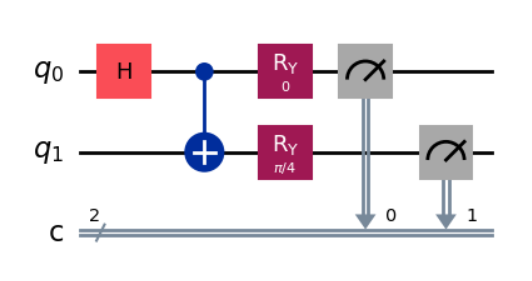
\includegraphics[width=\textwidth]{./img/Simulation/e91/image.png}
            \caption{Circuito de simulación de E91 para el par de bases ($\vec{a_{1}}, \vec{b_{1}}$)}
        \end{subfigure}
        \hfill
        \begin{subfigure}[t]{0.49\textwidth}
            \centering
            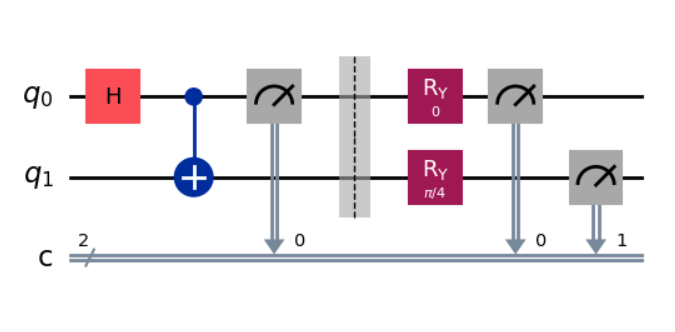
\includegraphics[width=\textwidth]{./img/Simulation/e91/image2.png}
            \caption{Circuito de simulación de E91 con Eve}
        \end{subfigure}
    \end{figure}\label{fig: circuito_simulacion_CHSH}

    \vspace{2.5mm}

    Donde se puede apreciar, en el lado izquierdo, el circuito de simulación sin Eve y a la derecha con Eve, en el que este espía mide el qubit de Alice previamente a su correspondiente medición, rompiendo así con el entrelazamiento y enviando dicho qubit a Bob. Es importante recalcar que este circuito se tomó para el par de bases \( (\vec{a_{1}}, \vec{b_{1}}) \), por lo que, partiendo del eje \textit{Z}, la base \( \vec{a_{1}} \) no necesita ninguna rotación (de ahí la rotación de 0), mientras que se aplica una rotación de \( \frac{\pi}{4} \) radianes sobre el eje \textit{Z} para obtener \( \vec{b_{1}} \). Este proceso se repite para cada par \( (\vec{a_{1}}, \vec{b_{1}}) \), sin embargo, se aplican rotaciones diferentes para cada caso, con el fin de medir en la base deseada correspondiente \( (\vec{a_{1}}, \vec{a_{3}}, \vec{b_{1}}, \vec{b_{3}}) \).

    \vspace{5mm}

    A continuación, se ha recopilado el resultado de las mediciones por cada par de bases en el siguiente gráfico, en el caso de que Eve no intercepte los qubits, con el que podremos deducir el valor de las correlaciones \( E(\vec{a_{i}}, \vec{b_{j}}) \):

    \begin{figure}[H]
        \centering
        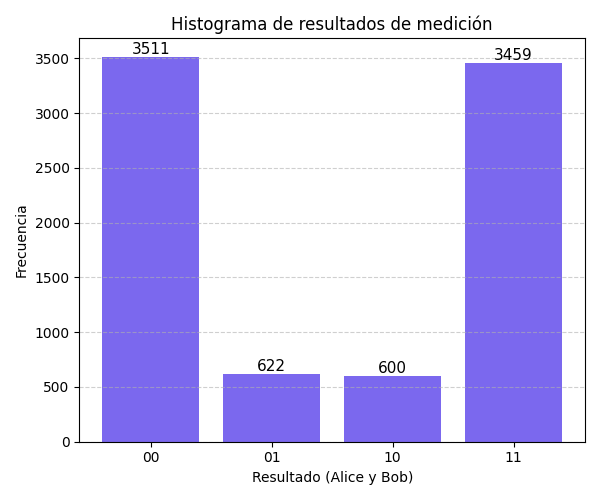
\includegraphics[width=0.95\textwidth]{./img/Simulation/e91/histograma_medidas.png}
        \caption{Histograma con los resultados de las mediciones de Alice y Bob}\label{fig: histograma_medidas}
    \end{figure}

    \vspace{2.5mm}

    Este gráfico tiene mucho sentido, ya que si calculamos teóricamente las correlaciones en cada par de bases \( E(\vec{a_{i}}, \vec{b_{j}}) \), obtenemos que

    \begin{equation}
        E(\vec{a_{1}}, \vec{b_{1}}) = \frac{\sqrt{2}}{2}, \quad E(\vec{a_{1}}, \vec{b_{3}}) = - \frac{\sqrt{2}}{2}, \quad E(\vec{a_{3}}, \vec{b_{1}}) = \frac{\sqrt{2}}{2}, \quad E(\vec{a_{1}}, \vec{b_{1}}) = \frac{\sqrt{2}}{2}
        \label{eq: correlaciones_teoricas_e91}
    \end{equation}

    \vspace{2.5mm}

    En este punto podemos ver que casi todas las correlaciones son positivas, lo que quiere decir que si Alice obtiene \( \ket{0} \) en su medición, es muy probable que obtenga \( \ket{0} \) al medir, y lo mismo aplica para \( \ket{1} \). Sin embargo, hay un resultado en el que obtenemos una correlación negativa para el par de bases \( (\vec{a_{1}}, \vec{b_{3}}) \), por lo que para esta base Alice y Bob obtendrán, en la mayoría de los casos, resultados opuestos al medir. Todo esto se puede ver reflejado en el gráfico (\ref{fig: histograma_medidas}), ya que para el par \( (\vec{a_{1}}, \vec{b_{3}}) \) predominan los estados \( \ket{01} \) y \( \ket{10} \), mientras que en el resto de casos, en los que la correlación es altamente positiva, predominan los estados \( \ket{00} \) y \( \ket{11} \).

    \vspace{5mm}

    Con esto podemos calcular el valor de las distintas correlaciones para cada par de bases \( E(\vec{a_{i}}, \vec{b_{j}}) \), tanto para el caso teórico como para el caso experimental, donde Eve realiza mediciones sobre los qubits y resetea el resultado de dichas mediciones a \( \ket{0} \). Las correlaciones están distribuidas en dos gráficos que reflejan ambos casos, a la izquierda sin Eve y a la derecha con la interceptación de Eve:

    \vspace{2.5mm}

    \begin{figure}[H]
        \begin{subfigure}[t]{0.49\textwidth}
            \centering
            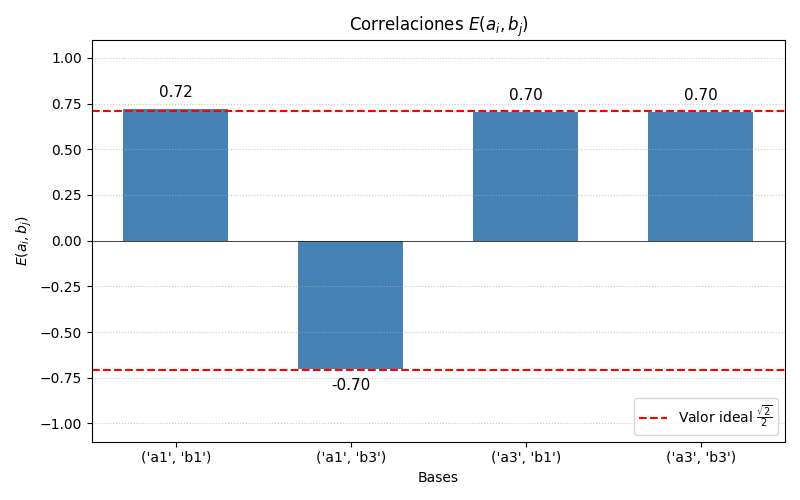
\includegraphics[width=\textwidth]{./img/Simulation/e91/corr_e91.png}
            \caption{Correlaciones \( E(a_{i}, b_{j}) \) sin Eve.}
        \end{subfigure}
        \hfill
        \begin{subfigure}[t]{0.49\textwidth}
            \centering
            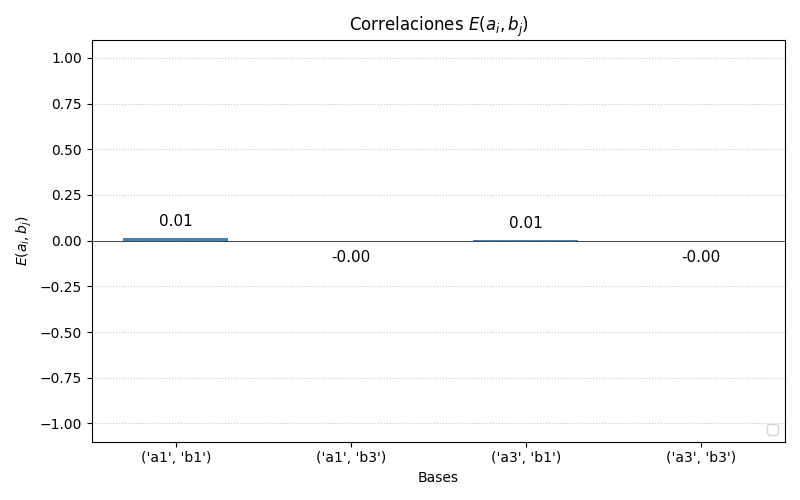
\includegraphics[width=\textwidth]{./img/Simulation/e91/corr_e91_eve.png}
            \caption{Correlaciones \( E(a_{i}, b_{j}) \) con Eve.}
        \end{subfigure}
    \end{figure}\label{fig: correlaciones_E91}

    \vspace{2.5mm}

    Se puede apreciar que, en el caso sin Eve, el resultado es bastante similar al esperado en la demostración teórica (\ref{eq: correlaciones_teoricas_e91}), en el que cada correlación \( E(\vec{a_{i}}, \vec{b_{j}}) \) alcanza un valor absoluto de \( \frac{\sqrt{2}}{2} \approx 0,7071\). Sin embargo, se puede observar que las correlaciones no son exactamente el valor teórico \( \frac{\sqrt{2}}{2} \). Esto sucede porque, aunque hagamos uso de un simulador sin ruido (\( \alpha = 0 \)), las correlaciones \( E(\vec{a_{i}}, \vec{b_{j}}) \) son una expectativa estadísitica en base al número de mediciones que realizan Alice y Bob, y esto es un número finito de mediciones, por lo que nunca van a ser exactamente el valor esperado \( \frac{\sqrt{2}}{2} \). No obstante, cuanto mayor sea el número de qubits compartidos entre Alice y Bob mayor será la convergencia a este resultado.

    \vspace{5mm}

    Por otra parte, en el caso de Eve las correlaciones son aproximadamente 0. Esto concuerda con nuestra explicación teórica, ya que si Eve rompe el entrelazamiento entre los qubits, los resultados de las mediciones dejarán de estar interconectados, rompiendo así cualquier correlación entre ellos. Esto es lo que significa la correlación \( E(\vec{a_{i}}, \vec{b_{j}}) = 0 \), un resultado completamente aleatorio al romper el entrelazamiento. En este punto, habiendo calculado todas las distintas correlaciones, podemos hallar el valor final de esta desigualdad \textit{CHSH}, \textit{S}, el cual bajo todo pronóstico resulta ser:

    \begin{figure}[H]
        \hspace{5mm}
        \begin{subfigure}[t]{0.40\textwidth}
            \centering
            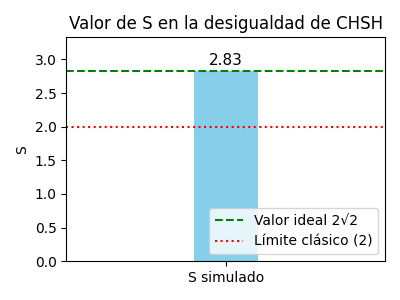
\includegraphics[width=\textwidth]{./img/Simulation/e91/s_e91.png}
            \caption{Valor final \textit{S} sin Eve.}
        \end{subfigure}
        \hfill
        \begin{subfigure}[t]{0.40\textwidth}
            \centering
            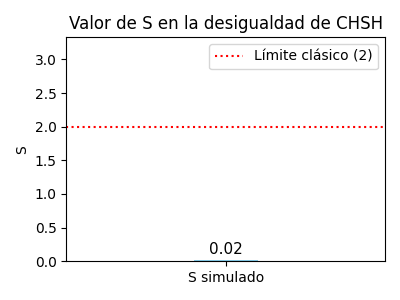
\includegraphics[width=\textwidth]{./img/Simulation/e91/s_e91_eve.png}
            \caption{Valor final \textit{S} bajo las interferencias causadas por Eve.}
        \end{subfigure}
        \hspace{5mm}
    \end{figure}\label{fig: valor_s_e91}

    \vspace{2.5mm}

    Esto es precisamente el resultado que esperábamos. Un valor de \textit{S} muy cercano al previsto en la teoría (\ref{eq: valor_correcto_s}) \( S = \frac{\sqrt{2}}{2} \approx 2,8284 \), siendo la diferencia con el resultado obtenido en la simulación muy pequeña y debida a la naturaleza estadística de las distintas correlaciones \( E(\vec{a_{i}}, \vec{b_{j}}) \) superando por el valor máximo el límite clásico, por lo que podemos concluir que los qubits de Alice y Bob se encontraban perfectamente entrelazados, como definimos en la simulación. De la misma manera sucede con Eve, siendo este valor muy próximo a 0 como efectivamente se esperaba, por lo que no se alcanza el límite clásico, concluyendo en que el entrelazamiento entre los qubits de Alice y Bob se ha visto perturbado y se verían obligados a repetir el protocolo debido a la presencia de Eve, el cual podría robar la clave de cifrado.

    \vspace{5mm}

    A modo de conclusión, el protocolo E91 propuesto por Artur Ekert~\cite{ekert_Original} se aprovecha de las propiedades del entrelazamiento mediante uno de los estados de Bell \( \ket{\Phi^{+}} \) para implementar un sistema de distribución de claves cuánticas \textit{QKD} de la manera más segura posible, siendo respaldado por la desigualdad \textit{CHSH}, mediante la cual podemos verificar el nivel de entrelazamiento real de los pares de qubits entre Alice y Bob, detectando así una intervención externa con la que se intente robar la clave de cifrado. Es por esto que el entrelazamiento es un recurso vital en la criptografía cuántica, ya que permite que la información se encuentre correctamente cifrada y segura frente a los ataques de Eve.

    \vspace{10mm}









    \newpage
    \thispagestyle{empty}
    \mbox{}

    \section{Algoritmos Cuánticos}\label{sec: algoritmos_cuanticos}

    \vspace{5mm}

    En este punto llegamos a una de las últimas secciones de este trabajo, en el que vamos a explicar y desarrollar por qué los ordenadores cuánticos son tan importantes. Todo se reduce a los algoritmos cuánticos, y es que, aprovechando las propiedades que ya sabemos como la superposición (\ref{eq: superposicion}) o entrelazamiento (\ref{sec: entrelazamiento_cuantico}) podemos mejorar la eficiencia de ciertos algoritmos, optimizándolos lo máximo posible, de manera que obtenemos algoritmos que en muchos casos son infinitamente más rápidos que la versión tradicional de estos procesos.

    \vspace{5mm}

    Cabe destacar que no todo algoritmo cuántico por ser cuántico, valga la redundancia, es más rápido, esto no siempre sucede así, pero como vimos anteriormente, toda información clásica se puede representar mediante un ordenador cuántico, por lo que únicamente tendríamos que clonar dichos procesos. En esta sección vamos seguir el plan propuesto en el libro escrito por \textit{Thomas G. Wong}~\cite{wong}, centrándonos en dos algoritmos: El algoritmo de Grover y el de Shor, los cuales mejoran la búsqueda por fuerza bruta y se optimiza de exponencial manera el problema de factorización, rompiendo con las claves públicas y privadas de ciertos cifrados como veremos próximamente.

    \vspace{5mm}





    \subsection{Oráculos Cuánticos}\label{subsection: oraculos_cuanticos}

    \vspace{5mm}

    Antes de comenzar por los oráculos, tenemos que explicar un par de conceptos. El primero es el de \textit{complejidad de circuitos}, ya que no todos los circuitos son iguales, podemos encontrar circuitos más o menos complejos que otros, y esto se mide contando el número mínimo de puertas cuánticas, tomando como referenca un conjunto de puertas cuánticas universales, como explicamos anteriormente al final de (\ref{subsubsection: la_puerta_de_toffoli}). Tomando como ejemplo el sumador cuántico require \( 32n - 14 \) puertas cuánticas, siendo \textit{n} el número de qubits que represetan a cada sumando en el sumador, y esto al depender de \textit{n}, decimos que tiene una complejidad lineal \textit{O(N)}.

    \vspace{5mm}

    Esto es lo que buscamos, ya que para que un algoritmo cuántico sea considerado eficiente ha de tener esta complejidad \textit{O(n)}. Sin embargo, hallar la complejidad de circuitos es una tarea muy difícil en muchos casos, y es por esto que se usan otros métodos, como el uso de \textit{oráculos cuánticos}. Esto es un método basado en la \textit{complejidad de consultas} (query complexity), de manera que tendremos una función, \( f(x) \) a la cual llamaremos un cierto número de veces, determinando así la complejidad \textit{O(N)}. 

    \vspace{5mm}

    Pongamos como ejemplo uno de los algoritmos que veremos a continuación, el \textit{algoritmo de Grover}. Este algoritmo mejora el problema de búsqueda por fuerza bruta de los computadores tradicionales, ya que en un computador clásico tenemos que explorar cada elemento uno a uno, y vemos si cumple con nuestros criterios. Si es el elemento que estamos buscando, el oráculo será \( f(x) = 1 \), y de lo contrario, si el oráculo es \( f(x) = 0 \) significa que no es el objeto que deseamos encontrar y que por lo tanto hemos de seguir buscando, siendo \( x \) el elemento consultado. Esto significa que, como hemos de consultar cada elemento uno a uno, tendremos una complejidad de \textit{O(N)} ya que en el peor de los casos tendremos que consultar la función oráculo \textit{N} veces, siendo \textit{N} el número total de elementos. Veremos posteriormente en (\ref{subsection: algoritmo_grover}) como reducimos la complejidad hasta \textit{O($\sqrt{N}$)}.

    \vspace{5mm}

    Esta idea aparece y se aplica en otros muchos otros algoritmos cuánticos, por lo que podemos asentar este concepto. Un oráculo cuántico no es más que una función booleana, es decir, su valor solo puede ser 0 o 1, lo que significa que puede definirse por medio de puertas lógicas convencionales. Si queremos tener un oráculo cuántico, tenemos que convertir este oráculo, el cual es un conjunto de puertas lógicas, en una puerta cuántica, y para ello debemos hacerla reversible como vimos en (\ref{subsection: puertas_cuanticas_de_1_qubit}). Esto se traduce a hacer que el oráculo sea reversible, y esto lo podemos hacer muy fácilmente, apoyándonos en una de las puertas lógicas más importantes, la puerta \textit{XOR}, cuya tabla de verdad es la siguiente:

    \vspace{2.5mm}

    \begin{figure}[H]
        \centering
        \renewcommand{\arraystretch}{1.5} % Espacio vertical aumentado
        \begin{tabular}{|>{\centering\arraybackslash}m{0.5cm}|>{\centering\arraybackslash}m{0.5cm}|>{\centering\arraybackslash}m{1.5cm}|}
            \hline
            A & B & A $\oplus$ B \\ \hline
            0 & 0 & 0 \\ \hline
            0 & 1 & 1 \\ \hline
            1 & 0 & 1 \\ \hline
            1 & 1 & 0 \\ \hline
        \end{tabular}
        \caption{Tabla de verdad de la puerta XOR}\label{fig:tabla_verdad_xor}
    \end{figure}

    \vspace{2.5mm}

    En definitiva, si añadimos un bit adicional \textit{y}, además del bit \textit{x} del oráculo, y pasamos ambos bits por una \textit{XOR}, obtendremos un resultado reversible que es lo que buscamos para que esto sea una puerta cuántica. Este nuevo oráculo reversible, lo hemos denotado como \( U_{f} \) en el siguiente circuito:

    \vspace{2.5mm}

    \begin{figure}[H]
        \[
        \Qcircuit @C=1em @R=1em {
            \lstick{\ket{x}} & \qw & \multigate{1}{\text{$ U_{f} $}} & \qw & \rstick{\ket{x}} \qw \\
            \lstick{\ket{y}} & \qw & \ghost{\text{$ U_{f} $}}        & \qw & \rstick{\ket{y \oplus f(x)}} \qw \\
        }
        \]
        \caption{Oráculo cuántico}
    \end{figure}

    \vspace{2.5mm}

    Actuando sobre \( \ket{x} \) y \( \ket{y} \) como sigue

    \begin{equation}
        \ket{x} \ket{y} \ \overset{U_{f}}{\longrightarrow} \ \ket{x} \ket{y \otimes f(x)}
        \label{eq: oraculo_cuantico}
    \end{equation}

    \vspace{2.5mm}

    Y este oráculo lo utilizaremos posteriormente en el algoritmo de Shor (\ref{subsection: algoritmo_shor}).

    \vspace{5mm}





    \subsection{Oráculo de Fase}

    \vspace{5mm}

    Lo siguiente que vamos a ver es el oráculo de fase, y está muy ligado a los oráculos cuánticos que acabamos de ver. Si nos fijamos en el oráculo de la sección anterior en (\ref{eq: oraculo_cuantico}), \( \ket{x} \) permanece intacto mientras que \( \ket{y} \) queda como \( \ket{y \otimes f(x)} \). En este caso queremos que el qubit que quede intacto sea \( \ket{y} \), quedando \( \ket{x} \) multiplicado por una fase, de ahí el nombre, oráculo de fase. Esto lo podemos lograr transformando \( \ket{y} \) en \( \ket{-} \), que lo podemos hacer inicializando \( \ket{y} \) en \( \ket{0} \), aplicando una puerta \textit{X}, es decir una puerta \textit{NOT}, y finalmente aplicando una puerta de Hadamard como sigue

    \begin{equation*}
        \ket{x} \ket{0} \ \overset{I \otimes X}{\longrightarrow} \ \ket{x} \ket{1} \ \overset{I \otimes H}{\longrightarrow} \ \ket{x} \ket{-}
    \end{equation*}

    \vspace{2.5mm}

    Entonces, si aplicamos el oráculo obtenemos lo que estábamos buscando, una fase multiplicando a \( \ket{x} \) y \( \ket{-} \) que permanece igual:

    \begin{align}
        \ket{x} \ket{-} &= \frac{1}{\sqrt{2}} \left( \ket{x} \ket{0} - \ket{x} \ket{1} \right) \overset{U_{f}}{\longrightarrow} \frac{1}{\sqrt{2}} \left( \ket{x} \ket{0 \oplus f(x)} - \ket{x} \ket{1 \oplus f(x)} \right) = \nonumber \\
        &= \begin{cases}
            \frac{1}{\sqrt{2}} \left( \ket{x} \ket{0} - \ket{x} \ket{1} \right), & f(x) = 0 \\[5pt]
            \frac{1}{\sqrt{2}} \left( \ket{x} \ket{1} - \ket{x} \ket{0} \right), & f(x) = 1 
        \end{cases} \nonumber \\
        &= \begin{cases}
            \ket{x} \ket{-}, & f(x) = 0 \\[5pt]
            -\ket{x} \ket{-}, & f(x) = 1
        \end{cases} \nonumber \\[5pt]
        &= (-1)^{f(x)} \ket{x} \ket{-}
        \label{eq: oraculo_fase}
    \end{align}

    \vspace{2.5mm}

    Y aquí tenemos el oráculo de fase en la expresión (\ref{eq: oraculo_fase}), en el que vemos que \( \ket{x} \) se encuentra multiplicado por la fase \( (-1)^{f(x)} \), la cual vemos que depende de \( f(x) \), mientras que el segundo qubit \( \ket{-} \) permanece igual. Esto lo vamos a usar en el siguiente apartado, en el que comenzaremos ya a explicar los algoritmos cuánticos que vamos a ver y su relación con la criptografía. 

    \vspace{5mm}






    \subsection{Algoritmo de Grover}\label{subsection: algoritmo_grover}

    \vspace{5mm}

    El primer ámbito de la criptografía que vamos a recorrer son los ataques mediante el uso de fuerza bruta. Esto ya lo explicamos anteriormente cuando definimos los oráculos cuánticos en (\ref{subsection: oraculos_cuanticos}) y básicamente se resume en que, según el algoritmo clásico, hemos de ir comprobando registro a registro si la información contenida es la que buscamos. Esto tiene una complejidad de \textit{O(N)} ya que, en el peor de los casos, la información que estamos buscando se encuentra en el último registro. Sin embargo, con el \textit{algoritmo de Grover}~\cite{grover_Original} vamos a lograr reducir dicha complejidad hasta \textit{O($ \sqrt{N} $)}.

    \vspace{5mm}

    Este algoritmo consta de \textit{n} qubits en el estado \( \ket{+} \), lo cual denotaremos por \( \ket{+}^{\otimes n} \), y el qubit \( \ket{y} \) para poder aplicar el oráculo de fase, el cual se encontrará inicialmente en \( \ket{-} \). Vamos a comenzar denotando todos estos estos qubits en \( \ket{+}^{\otimes n} \) como \( \ket{s} \):

    \begin{gather*}
        \ket{0}^{\otimes n} \ \overset{H \otimes n}{\longrightarrow} \ \ket{+}^{\otimes n} \\[5pt]
        \ket{s} = \ket{+}^{\otimes n} = \left( \frac{1}{\sqrt{2}} \right)^{n} \left( \ket{0} + \ket{1} \right)^{\otimes n} = \frac{1}{\sqrt{2^{n}}} \sum_{x \in \{ 0,1 \}^{n}} \ket{x}
    \end{gather*}

    \vspace{2.5mm}

    Y \( 2^{n} \) es el número total de registros que vamos a tener en nuestra base de datos, ya que \textit{n} es el número de bits que tienen nuestras cadenas de datos. Es por esto que vamos a denotar \( 2^{n} = N \), quedando

    \begin{equation}
        \ket{s} = \frac{1}{\sqrt{N}} \sum_{x \in \{ 0,1 \}^{n}} \ket{x}
        \label{eq: estado_s_algoritmo_grover}
    \end{equation}

    \vspace{2.5mm}

    Entonces, el dato que estamos buscando será una de las posibles cadenas que estamos consultando. A este dato el cual es nuestro objetivo ya que es el que queremos encontrar, lo vamos a denotar como \( \ket{w} \), y al resto de cadenas que son irrelevantes, \( \ket{i} \). Esto lo podemos llevar a (\ref{eq: estado_s_algoritmo_grover}), y desarrollando la expresión, llegamos a

    \begin{align}
        \ket{s} &= \frac{1}{\sqrt{N}} \left( \ket{w} + \sum_{i \neq w} \ket{i} \right) = \frac{1}{\sqrt{N}} \ket{w} + \frac{1}{\sqrt{N}} \sum_{i \neq w} \ket{i} = \nonumber \\[5pt]
        &= \frac{1}{\sqrt{N}} \ket{w} + \sqrt{\frac{N - 1}{N}} \frac{1}{\sqrt{N - 1}} \sum_{i \neq w} \ket{i} = \frac{1}{\sqrt{N}} \ket{w} + \sqrt{\frac{N - 1}{N}} \ket{r}
        \label{eq: desarrollo_s_algoritmo_grover}
    \end{align}

    \vspace{2.5mm}

    De donde

    \begin{equation*}
        \ket{r} = \frac{1}{\sqrt{N - 1}} \sum_{i \neq w} \ket{i} 
    \end{equation*}

    \vspace{2.5mm}

    Siendo \( \ket{r} \) una superposición de todos los estados \( \ket{i} \) que no son la solución que estamos buscando. Además \( \ket{r} \) es una superposición que está normalizada, ya que hemos dividido entre \( \sqrt{N - 1} \) al haber \( N - 1 \) términos en el sumatorio. Sin embargo podemos desarollar la expresión (\ref{eq: desarrollo_s_algoritmo_grover}) aún un poquito más, y es que si nos fijamos dicha expresión es muy similar a la descomposición de un vector en componentes ortogonales, las cuales son \( \ket{w} \) y \( \ket{r} \). Es por esto que podemos extrapolar dicha expresión a un plano de coordenadas en función de un ángulo $ \theta $, donde los ejes son \( \ket{w} \) y \( \ket{r} \):

    \begin{equation}
        \ket{s} = \frac{1}{\sqrt{N}} \ket{w} + \sqrt{\frac{N - 1}{N}} \ket{r} = \sin \theta \ket{w} + \cos \theta \ket{r}
    \end{equation}

    \vspace{2.5mm}

    Con \( \theta \) definido como

    \begin{equation*}
        \sin \theta = \frac{1}{\sqrt{N}}, \qquad \cos \theta = \sqrt{\frac{N - 1}{N}}
        \label{eq: theta_grover}
    \end{equation*}

    \vspace{2.5mm}

    Lo cual es consistente con las entidades trigonométricas:

    \begin{gather*}
        \sin^{2} \theta + \cos^{2} \theta = 1 \\[5pt]
        \left( \frac{1}{\sqrt{N}} \right)^{2} + \left( \sqrt{\frac{N - 1}{N}} \right)^{2} = \frac{1 + N - 1}{N} = 1
    \end{gather*}

    \vspace{2.5mm}

    Entonces, podemos llevarnos todo esto al plano que acabamos de definir en función de \( \ket{w} \) y \( \ket{r} \):

    \vspace{2.5mm}

    \begin{figure}[H]
        \centering
        \begin{tikzpicture}[>=Stealth, scale=2.5]
            % Configuración global
            \def\axislength{1.5}   % Longitud de los ejes (para |r⟩ y |w⟩)
            \def\thetangle{10}     % Ángulo θ entre |s⟩ y |r⟩ (sin mostrar valor)
            
            % Ejes (vectores |r⟩ y |w⟩)
            \draw[->, thick, black] (0,0) -- (\axislength,0) node[right]{$ \ket{r} $};
            \draw[->, thick, black] (0,0) -- (0,\axislength) node[above]{$ \ket{w} $};
            
            % Vector |s⟩ (unitario, ángulo θ)
            \draw[->, thick, red] (0,0) -- ({\thetangle}:1.5) node[above right]{$ \ket{s} $};
            
            % Ángulo θ (arco sin valor numérico)
            \draw (0.5,0) arc (0:\thetangle:0.5);
            \node at ({\thetangle/2}:0.7) {$\theta$};    
        \end{tikzpicture}
        \caption{Representación de $ \ket{s} $ en el plano}\label{fig: s_plano}
    \end{figure}

    \vspace{2.5mm}

    Ahora es cuando viene el momento de aplicar el oráculo de fase. Para ello necesitamos el qubit \( \ket{y} \), el cual asumiremos que se encuentra directamente en \( \ket{-} \). Entonces, aplicando el oráculo, obtenemos:

    \begin{gather*}
        \ket{s} \ket{-} \ \overset{U_{f}}{\longrightarrow} \ \left[ (-1)^{f(x)} \ket{s} \right] \ket{-} = \left[ (-1)^{f(x)} \left( \sin \theta \ket{w} + \cos \theta \ket{r} \right) \right] \ket{-} = \\[5pt]
        = \left( (-1)^{f(x)} \sin \theta \ket{w} + (-1)^{f(x)} \cos \theta \ket{r} \right) \ket{-}
    \end{gather*}

    \vspace{2.5mm}

    Y el valor de \( f(x) \) sabemos que es un valor binario al ser una función booleana, y su valor es 1 cuando verificamos que el dato que estamos analizando es la solución que estamos buscando \( \ket{x} = \ket{w} \), y 0 en caso contrario. Sabiendo esto, llegamos a

    \begin{equation*}
        \left( (-1)^{1} \sin \theta \ket{w} + (-1)^{0} \cos \theta \ket{r} \right) \ket{-} = \left( - \sin \theta \ket{w} + \cos \theta \ket{r} \right) \ket{-}
    \end{equation*}

    \vspace{2.5mm}

    De donde \( \ket{s} \) tras aplicar el oráculo de fase es

    \begin{equation}
        U_{f} \ket{s} = - \sin \theta \ket{w} + \cos \theta \ket{r}
    \end{equation}

    \vspace{2.5mm}

    Y esto en definitiva es una reflexión \( U_{f} \ket{s} \) de \( \ket{s} \) sobre \( \ket{r} \):

    \vspace{2.5mm}

    \begin{figure}[H]
        \centering
        \begin{tikzpicture}[>=Stealth, scale=2.5]
            % Configuración global
            \def\axislength{1.5}   % Longitud de los ejes (para |r⟩ y |w⟩)
            \def\thetangle{10}     % Ángulo θ entre |s⟩ y |r⟩ (sin mostrar valor)
            
            % Ejes (vectores |r⟩ y |w⟩)
            \draw[->, thick, black] (0,0) -- (\axislength,0) node[right]{$ \ket{r} $};
            \draw[->, thick, black] (0,0) -- (0,\axislength) node[above]{$ \ket{w} $};
            
            % Vector |s⟩ (unitario, ángulo θ)
            \draw[->, thick, red] (0,0) -- ({\thetangle}:1.5) node[above right]{$ \ket{s} $};
            \draw[->, thick, red] (0,0) -- (-{\thetangle}:1.5) node[below right]{$ U_{f} \ket{s} $};
            
            % Ángulo θ (arco sin valor numérico)
            \draw (0.5,0) arc (0:\thetangle:0.5);
            \node at ({\thetangle/2}:0.7) {$\theta$}; 
            \draw (0.5,0) arc (0:-\thetangle:0.5);
            \node at (-{\thetangle/2}:0.7) {$\theta$};    
        \end{tikzpicture}
        \caption{Reflexión $ U_{f} \ket{s} $ en el plano}\label{fig: ufs_plano}
    \end{figure}

    \vspace{2.5mm}

    Ahora viene una parte muy interesante de este algoritmo. Para poder explicarla correctamente vamos a definir el operador de reflexión sobre \( \ket{s} \), el cual es una puerta cuántica \( R_{s} \) que tiene la siguiente forma:

    \begin{equation}
        R_{s} = 2 \ket{s} \bra{s} - I
        \label{eq: reflexion_sobre_s}
    \end{equation}

    \vspace{2.5mm}

    Esta es la reflexión sobre \( \ket{s} \). Para iluminarnos un poco más, si aplicamos esta puerta cuántica sobre \( \ket{s} \) nos debería dar como resultado el propio estado \( \ket{s} \)

    \begin{equation*}
        R_{s} \ket{s} = \left( 2 \ket{s} \bra{s} - I \right) \ket{s} =  2 \ket{s} \braket{s | s} - \ket{s} = 2 \ket{s} - \ket{s} = \ket{s} 
    \end{equation*}

    \vspace{2.5mm}

    Donde \( \braket{s | s} = 1 \), como vimos en (\ref{eq: producto_escalar_vector_mismo_l2}). De la misma manera si aplicamos \( R_{s} \) sobre un vector un vector ortogonal a \( \ket{s} \), \( \ket{s^{\perp}} \), el resultado debería ser el mismo vector ortogonal \( \ket{s^{\perp}} \) cambiado de signo, es decir \( - \ket{s^{\perp}} \)

    \begin{equation*}
        R_{s} \ket{s^{\perp}} = \left( 2 \ket{s} \bra{s} - I \right) \ket{s^{\perp}} =  2 \ket{s} \braket{s | s^{\perp}} - \ket{s^{\perp}} = - \ket{s^{\perp}} 
    \end{equation*}

    \vspace{2.5mm}

    Por lo que ya podemos deducir de una manera intuitiva que efectivamente \( R_{s} \) es un operador de reflexión sobre \( \ket{s} \). Nos queda demostrar que se trata de una puerta cuántica, y para ello vamos a ver que es una matriz unitaria, definiendo en primer lugar que el conjugado hermítico \( R_{s}^{\dagger} \) es igual a \( R_{s} \):
    
    \begin{equation*}
        R_{s}^{\dagger} = \left( 2 \ket{s} \bra{s} - I \right)^{\dagger} = 2 \ket{s} \bra{s} - I = R_{s}  
    \end{equation*}

    \vspace{2.5mm}

    Entonces ya podemos aplicar la expresión vista en (\ref{eq: puertas_cuanticas_unitarias}), en la que vamos a ver que \( R_{s}^{\dagger} R_{s} \) es la matriz identidad:

    \begin{align*}
        R_{s}^{\dagger} R_{s} &= R_{s} R_{s} = \left( 2 \ket{s} \bra{s} - I \right) \left( 2 \ket{s} \bra{s} - I \right) = 4 \ket{s} \braket{s | s} \bra{s} - 4 \ket{s} \bra{s} + I = \\[5pt] 
        &= 4 \ket{s} \bra{s} - 4 \ket{s} \bra{s} + I = I
    \end{align*}

    \vspace{2.5mm}

    Por lo que \( R_{s} \) es una puerta cuántica, como queríamos demostrar. Siguiendo con el algoritmo, vamos a aplicar el operador de reflexión \( R_{s} \) (\ref{eq: reflexion_sobre_s}) sobre \( U_{f} \ket{s} \), lo cual podemos ver el plano de la siguiente manera, denotado como \( R_{s} U_{f} \ket{s} \):

    \vspace{2.5mm}

    \begin{figure}[H]
        \centering
        \begin{tikzpicture}[>=Stealth, scale=2.5]
            % Configuración global
            \def\axislength{1.5}   % Longitud de los ejes (para |r⟩ y |w⟩)
            \def\thetangle{10}     % Ángulo θ entre |s⟩ y |r⟩ (sin mostrar valor)
            \def\doubletheangle{30}
            \def\nodeangle{40}
            
            % Ejes (vectores |r⟩ y |w⟩)
            \draw[->, thick, black] (0,0) -- (\axislength,0) node[right]{$ \ket{r} $};
            \draw[->, thick, black] (0,0) -- (0,\axislength) node[above]{$ \ket{w} $};
            
            % Vector |s⟩ (unitario, ángulo θ)
            \draw[->, thick, red] (0,0) -- ({\thetangle}:1.5) node[above right]{$ \ket{s} $};
            \draw[->, thick, red] (0,0) -- (-{\thetangle}:1.5) node[below right]{$ U_{f} \ket{s} $};

            \draw[->, thick, blue] (0,0) -- ({\doubletheangle}:1.5) node[above right]{$ R_{s} U_{f} \ket{s} $};
            
            % Ángulo θ (arco sin valor numérico)
            \draw (0.5,0) arc (0:\thetangle:0.5);
            \node at ({\thetangle/2}:0.7) {$\theta$}; 
            \draw (0.5,0) arc (0:-\thetangle:0.5);
            \node at (-{\thetangle/2}:0.7) {$\theta$};   
            \draw (0.5,0) arc (0:\doubletheangle:0.5);
            \node at ({\nodeangle/2}:0.7) {$2 \theta$};  
        \end{tikzpicture}
        \caption{Reflexión $ R_{s} U_{f} \ket{s} $ en el plano}\label{fig: rsufs_plano}
    \end{figure}    

    \vspace{2.5mm}

    Y si vamos aplicando el oráculo \( U_{f} \) y la reflexión \( R_{s} \), seguimos rotando con un ángulo de \( 2 \theta \) hasta converger a la solución \( \ket{w} \)

    \vspace{2.5mm}

    \begin{figure}[H]        
        \centering
        \begin{tikzpicture}[>=Stealth, scale=2.5]
            % Configuración global
            \def\axislength{1.5}   % Longitud de los ejes (para |r⟩ y |w⟩)
            \def\thetangle{10}     % Ángulo θ entre |s⟩ y |r⟩ (sin mostrar valor)
            \def\doubletheangle{30}
            \def\nodeangle{40}            
            \def\tripletheangle{50}
            \def\triplenodeangle{80}

        
            % Ejes (vectores |r⟩ y |w⟩)
            \draw[->, thick, black] (0,0) -- (\axislength,0) node[right]{$ \ket{r} $};
            \draw[->, thick, black] (0,0) -- (0,\axislength) node[above]{$ \ket{w} $};
            
            % Vector |s⟩ (unitario, ángulo θ)
            \draw[->, thick, red] (0,0) -- ({\thetangle}:1.5) node[above right]{$ \ket{s} $};
            \draw[->, thick, red] (0,0) -- (-{\thetangle}:1.5) node[below right]{$ U_{f} \ket{s} $};

            \draw[->, thick, blue] (0,0) -- ({\doubletheangle}:1.5) node[above right]{$ R_{s} U_{f} \ket{s} $};
            \draw[->, thick, blue] (0,0) -- ({\tripletheangle}:1.5) node[above right]{$ (R_{s} U_{f})^{2} \ket{s} $};
            
            % Ángulo θ (arco sin valor numérico)
            \draw (0.5,0) arc (0:\thetangle:0.5);
            \node at ({\thetangle/2}:0.7) {$\theta$}; 
            \draw (0.5,0) arc (0:-\thetangle:0.5);
            \node at (-{\thetangle/2}:0.7) {$\theta$};   
            \draw (0.5,0) arc (0:\doubletheangle:0.5);
            \node at ({\nodeangle/2}:0.7) {$2 \theta$}; 
            \draw (0.5,0) arc (0:\tripletheangle:0.5);
            \node at ({\triplenodeangle/2}:0.7) {$2 \theta$};  
        \end{tikzpicture}
        \caption{Segunda reflexión $ (R_{s} U_{f})^{2} \ket{s} $ en el plano}\label{fig: rsuf2s_plano}
    \end{figure}  

    \vspace{2.5mm}

    Vamos a suponer que tenemos que aplicar esta reflexión un total de \( t \) veces, podemos hallar este valor \( t \) en función de \( \theta \), de la siguiente manera, sabiendo que el ángulo definido entre \( \ket{w} \) y \( \ket{r} \) es \( \frac{\pi}{2} \):

    \begin{gather*}
        \theta + t \left( 2 \theta \right) = \frac{\pi}{2} \\[5pt]
        t \left( 2 \theta \right) = \frac{\pi}{2} - \theta \\[5pt]   
        t = \frac{\pi}{4 \theta} - \frac{1}{2}  
    \end{gather*}

    \vspace{2.5mm}

    Y a su vez \( \theta \) depende del número total de registros \textit{N} a los que estamos aplicando este algoritmo de fuerza bruta:

    \begin{gather*}
        \theta = \sin^{-1} \left( \frac{1}{\sqrt{N}} \right) \approx \frac{1}{\sqrt{N}}
    \end{gather*}

    \vspace{2.5mm}

    Esto lo hemos obtenido de (\ref{eq: theta_grover}), y hemos asumido que \textit{N} es grande, obteniendo el resultado, que aunque sea una aproximación, es bastante firme y que no necesita depender de un valor tan elevado de \textit{N}. Entonces, podemos concluir que el número de iteraciones o llamadas sobre el oráculo de fases es:

    \begin{equation}
        t \approx \frac{\pi}{4} \sqrt{N} - \frac{1}{2} \approx \frac{\pi}{4} \sqrt{N}
    \end{equation}

    \vspace{2.5mm}

    Lo cual es lo que estábamos buscando, determinándose una complejidad de \( O(\sqrt{N}) \) para este algoritmo ya que precisamos de un número dependiente de \( \sqrt{N} \) llamadas al oráculo de fases, hasta converger en \( \ket{w} \). Es con este algoritmo que conseguimos reducir la complejidad del algoritmo de fuerza bruta clásico, y el salto de \textit{N} a \( \sqrt{N} \) llamadas al oráculo se denomina como \textit{aceleración cuadrática}, y esto es posible gracias a un proceso iterativo, en el vamos aplicando el operador de reflexión \( R_{s} \), con el que conseguimos una rotación en el espacio de Hilbert \( \mathcal{H} \) hasta converger a la solución \( \ket{w} \), lo cual es posible gracias a un oráculo muy eficiente y con el que aprovechamos las propiedades de la mecánica cuántica.

    \vspace{5mm}





    \subsection{El Algoritmo de Shor}\label{subsection: algoritmo_shor}

    \vspace{5mm}

    \subsubsection{RSA}\label{subsubsection: rsa}

    \vspace{5mm}

    Clásicamente, el sistema que se suele seguir para encriptar y desencriptar mensajes se basa en claves públicas y privadas, con las que encriptamos y desencriptamos la información, respectivamente. Hay muchos sistemas basados en este principio, aunque nos vamos a centrar en el criptosistema \textit{RSA}, el cual surgió en 1977 y se aprovecha de este enfoque. 

    \vspace{5mm}

    Este sistema se basa en la factorización de números muy grandes, ya que este es uno de los problemas de los computadores convencionales al ser una tarea computacionalmente bastante costosa, resultando prácticamente imposible la factorización de ciertos números para un ordenador clásico. Este es un protocolo de vital importancia y que se usa hoy día, sin embargo, con el \textit{algoritmo de Shor} (\ref{subsubsection: algoritmo_shor}) veremos que esta tarea, para un ordenador cuántico, es mucho menos costosa.

    \vspace{5mm}

    Aunque esto no es un algoritmo cuántico, está incluido en esta sección para explicar y comprender de una mejor manera el algoritmo de Shor, el cual veremos posteriormente. Imaginemos un emisor, Alice, que quiere enviar un mensaje a un receptor Bob. Para ello, Bob prepara una clave pública, la cual será accesible para todo el mundo y que permitirá a cualquier emisor enviarle un mensaje, y de la misma manera, Bob crea una clave privada, la cual es accesible únicamente por Bob, para desencriptar los mensajes de Alice.

    \vspace{5mm}

    El primer paso es escoger dos números primos, \textit{p} y \textit{q}, los cuales han de seguir ciertas condiciones, entre las cuales vamos a resumir que han de ser dos números primos con aproximadamente 1024 bits en lenguaje binario. Esto es, para que al multiplicarlos entre ellos, obtengamos un resultado \textit{n} de 2048 bits, el cual será la primera de las dos claves públicas de Bob. Esto se rige en base al estándar RSA actual, en el cual se establece que para que nuestra información sea completamente segura, el producto de los dos números primos escogidos por Bob ha de tener 2048 bits en binario, para que sea un sistema inquebrantable por un ordenador clásico, aunque deje bastante que desear para un computador cuántico. 

    \begin{equation}
        n = p q
        \label{eq: obtencion_n_RSA}
    \end{equation}

    \vspace{2.5mm}

    A continuación vamos a establecer la segunda clave pública. Para ello calculamos 

    \begin{equation}
        \phi = (p - 1) (q - 1)
        \label{eq: phi_RSA}
    \end{equation}

    \vspace{2.5mm}

    Y posteriormente hemos de encontrar un entero \textit{e} cuyo máximo común divisor con \( \phi \) sea igual a 1, sto significa que \textit{e} y \( \phi \) son coprimos:

    \begin{equation}
        \text{gcd} (e, \phi) = 1, \qquad e \in \mathbb{Z}
    \end{equation}

    \vspace{2.5mm}

    Hay muchos métodos que nos permiten obtener un valor de \textit{e}, como el algoritmo de euclides. En definitiva, \textit{e} es la segunda clave pública de Bob. Continuando con este protocolo, vamos a hallar la clave privada de Bob, la cual es 

    \begin{equation}
        e \cdot d \equiv 1 \ \text{mod} \ \phi
    \end{equation}

    \vspace{2.5mm}

    Esta será nuestra clave privada \textit{d}, cual multiplicada por una de las claves públicas \textit{e}, da como resultado la unidad módulo \( \phi \). Esta clave \textit{d} permitirá a Bob desencriptar cualquier mensaje encriptado por Alice, y será una clave muy segura ya que para hallar \textit{d} hemos de conocer el valor de \( \phi \), el cual se estableció en (\ref{eq: phi_RSA}) y que depende de dos números primos \textit{p} y \textit{q}, por lo que si queremos conocer el valor de \textit{d}, es necesario aplicar un algoritmo de factorización, y los ordenadores clásicos en esta tarea son muy ineficientes.

    \vspace{5mm}

    Es ahora el momento en el que Alice envía un mensaje a Bob, el cual denotaremos como \textit{M} y será un mensaje binario menor que la primera clave pública de Bob, \textit{N}, por lo que \( 0 < M < n \). Para enviar el mensaje cifrado a Bob, utiliza sus claves públicas \textit{n} y \textit{e} de manera que el mensaje codificado \textit{C} queda como

    \begin{equation*}
        C = M^{e} \ \text{mod} \ n
    \end{equation*}

    \vspace{2.5mm}

    Y, una vez el mensaje es enviado cifrado a Bob, este solo tiene que desencriptarlo utilizando su clave privada \textit{d}, a través del siguiente proceso:

    \begin{equation*}
        C^{d} \ \text{mod} \ n = (M^{e})^{d} \ \text{mod} \ n = M^{ed} \ \text{mod} \ n = M^{1} \ \text{mod} \ n = M 
    \end{equation*}

    \vspace{2.5mm}

    Por lo que Bob ha recibido el mensaje de Alice correctamente. Este protocolo nos ayuda a entender de una mejor manera por qué un algoritmo de factorización eficiente es tan importante, ya que podríamos hallar el valor de \( \phi \) muy rápidamente, y por lo tanto, tendríamos la clave privada \textit{d} en nuestro poder, descifrando cualquier información enviada a Bob. Vamos a ver una forma de romper esta factorización con el algoritmo de Shor (\ref{subsubsection: algoritmo_shor}), el cual vamos a ver a continuación en el siguiente apartado.

    \vspace{5mm}





    \subsubsection{Algoritmo de Shor}\label{subsubsection: algoritmo_shor}

    \vspace{5mm}

    En 1994 llegó una revolución para la criptografía cuántica. Fue gracias a \textit{Peter Shor} y a su revolucionario algoritmo cuántico~\cite{shor_Original} con el que se rompen las bases de la criptografía pública y privada mediante la mejora del algoritmo de factorización por números primos clásico. Es por esto que ciertos sistemas, como el protocolo \textit{RSA} (\ref{subsubsection: rsa}), ya no son tan robustos frente a un ordenador cuántico. Para comenzar con el algoritmo, se parte de la tarea de factorizar el entero \( N \). 

    \vspace{5mm}

    Para este algoritmo se van a aplicar muchas de las condiciones vistas en otros métodos de cifrado clásicos, como \textit{RSA} (\ref{subsubsection: rsa}) en el que se explicó el máximo común divisor \textit{gcd}, expresiones modulares, y se estudió con un leve nivel de detalle las propiedades de la teoría de números aplicadas a los números coprimos. Es en esto, y con la ayuda de ciertos algoritmos cuánticos, en lo que se basa el algoritmo de Shor para factorizar un \( N \in \mathbb{Z} \) en dos números primos \textit{p} y \textit{q}. Según el libro escrito por \textit{Thomas G. Wong}~\cite{wong}, este proceso puede dividirse en tres partes:

    \vspace{2.5mm}

    \begin{enumerate}

        \item Escogemos un número \( a \in \mathbb{Z} \) tal que \( 1 < a < N \), siendo \( N \) el número que deseamos factorizar. A continuación calculamos el máximo común divisor entre \textit{a} y \textit{N} y, si \( gcd(a, N) \neq 1 \), esto quiere decir que \textit{a} y \textit{N} comparten un divisor no trivial, por lo que uno de los factores que estamos buscando es \( p = gcd(a, N) \), y el otro lo podemos obtener en base a este factor, ya que este es \( q = N / p \), y finalizaría el algoritmo.  Si por el contrario \( gcd(a, N) = 1 \) quiere decir que \textit{a} y \textit{N} son coprimos, por lo que no comparten ningún divisor en común. En este caso no podemos encontrar los factores directamente y hemos de proceder con el siguiente paso del algoritmo.
        
        \vspace{5mm}

        En definitiva el objetivo de este primer paso es inicializar \textit{a} y ver si se da la casualidad de que este número comparta algún divisor no trivial con \textit{N}, lo cual no suele ser algo común ya que se asume que \textit{N} es un número muy grande, y por tanto no podemos aplicar ningún método clásico para obtener \textit{a} de manera que \( gcd(a, N) \neq 1 \). Lo más normal es que tengamos que recurrir al siguiente paso. 

        \vspace{5mm}

        \item Encontrar el periodo modular \textit{r} de \( a^{x} \ \text{mod} \ N \). Supongamos que \textit{a} tiene un valor de 7, y \textit{N = 15}. La variable \textit{x} toma valores \(x \in \{ 0, 1, 2, \cdots \} \) de manera que
        
        \begin{align*}
            7^{0} \ \text{mod} 15 &= 1 \ \text{mod} \ 15 = 1\\[5pt]
            7^{1} \ \text{mod} 15 &= 7 \ \text{mod} \ 15 = 7\\[5pt]
            7^{2} \ \text{mod} 15 &= 49 \ \text{mod} \ 15 = 4\\[5pt]
            7^{3} \ \text{mod} 15 &= 354 \ \text{mod} \ 15 = 13 \\[5pt]
            7^{4} \ \text{mod} 15 &= 2401 \ \text{mod} \ 15 = 1
        \end{align*}

        \vspace{2.5mm}

        Y si seguimos incrementando el valor de \textit{x}, este ciclo se repite, ya que 7 y 15 son coprimos. El periodo \textit{r} es el menor entero positivo (mayor que cero) con el que se verifica esta secuencia, por lo que en este caso, el periodo es \textit{r = 4} como podemos ver. Esta operación resulta ser muy ineficiente para un ordenador clásico, pero bastante más eficiente para un ordenador que se apoye en las leyes de la mecánica cuántica, y el algoritmo cuántico que resuelve esta operación necesita estimar el autovalor de ciertos autovectores, lo cual cubrimos en (\ref{subsubsection: estimacion_autovalores}).

        \vspace{5mm}

        Una vez hemos averiguado el valor de \textit{r}, este ha de cumplir una serie de condiciones. La primera es que \textit{r} ha de ser un número par, y la segunda es \( a^{r / 2} \ \text{mod} \ N \neq N - 1 \). En el caso incumplirse alguna de estas restricciones, volvemos al primer paso, escogemos un valor distinto para \textit{a} y repetimos el proceso desde el principio.
        
        \vspace{5mm}

        \item A continuación explicamos el último paso, con el cual vamos a obtener los factores primos \textit{p} y \textit{q} de \textit{N}. En primer lugar, necesitamos expresar \textit{r} en función de un múltiplo de \textit{N}, esto lo podemos conseguir muy fácilmente
        
        \begin{gather*}
            a^{r} = 1 \ \text{mod} \ N \\[5pt]
            a^{r} - 1 = 0 \ \text{mod} \ N \\[5pt]
            a^{r} - 1 = k N
        \end{gather*}

        \vspace{2.5mm}

        Donde \( k \in \mathbb{Z} \) es un múltiplo de \textit{N}. No obstante el objetivo de este problema es hallar \textit{p} y \textit{q}, por lo que expresamos \textit{N} en función de ellos, y además, podemos factorizar el término \( a^{r} - 1 \) como sigue

        \begin{equation*}
            \left( a^{r / 2} + 1 \right) \left( a^{r / 2} - 1 \right) = k p q
        \end{equation*}

        \vspace{2.5mm}

        Esto lo podemos hacer porque hemos definido anteriormente en el segundo paso que \textit{r} ha de ser un número par, para que los factores \( a^{r / 2} + 1 \) y \( a^{r / 2} - 1 \) sean números enteros, ya que si no pertenecen a este conjunto, sería mucho más difícil, por no decir imposible, esta factorización. Llegados a este punto, \textit{p} o \textit{q} deben estar incluidos en al menos uno de los términos \( a^{r / 2} + 1 \) o \( a^{r / 2} - 1 \), lo que nos conduce a estas tres posibilidades:

        \begin{gather}
            \underbrace{ \left( a^{r / 2} + 1 \right)}_{c} \underbrace{ \left( a^{r / 2} - 1 \right)}_{dpq} = k p q \nonumber \\[5pt]
            \underbrace{ \left( a^{r / 2} + 1 \right)}_{cp} \underbrace{ \left( a^{r / 2} - 1 \right)}_{dq} = k p q\label{eq: posible_caso_shor} \\[5pt]
            \underbrace{ \left( a^{r / 2} + 1 \right)}_{cpq} \underbrace{ \left( a^{r / 2} - 1 \right)}_{d} = k p q \nonumber
        \end{gather}

        \vspace{2.5mm}

        Donde \( k = cd \). Sin embargo, el primer y el tercer caso son imposibles ya que \( a^{r / 2} + 1 \) y \( a^{r / 2} - 1 \) no son en ningún caso múltiplos de \textit{N}. Esto es posible gracias a las condiciones definidas en el segundo paso, con las cuales obtenemos que \( a^{r / 2} \neq N - 1 \ \text{mod} \ N \) además de \( a^{r / 2} \neq 1 \ \text{mod} \ N \) gracias a la definición del periodo \textit{r}. Es por esto que descartamos la primera y tercera opción, quedándonos únicamente con (\ref{eq: posible_caso_shor}):

        \begin{equation*}
            \underbrace{ \left( a^{r / 2} + 1 \right)}_{cp} \underbrace{ \left( a^{r / 2} - 1 \right)}_{dq} = k p q \\[5pt]
        \end{equation*}

        \vspace{2.5mm}

        Entonces, ambos términos \( a^{r / 2} + 1 \) y \( a^{r / 2} - 1 \) contienen un factor no trivial de \textit{N}, y los podemos calcular con el máximo común divisor (\textit{gcd}):
        
        \begin{align*}
            p &= \gcd(a^{r / 2} + 1, N) \\[5pt]
            q &= \gcd(a^{r / 2} + 1, N)
        \end{align*}

        \vspace{2.5mm}

    \end{enumerate}

    Obteniendo así la descomposición de \textit{N} en los factores primos \textit{p} y \textit{q}. Este algoritmo es posible gracias a la obtención del periodo \textit{r}, ya que este proceso es exponencialmente más rápido mediante un ordenador cuántico que con un computador clásico, lo que muestra muy claramente el poder de la computación cuántica en la rama de la seguridad informática, surgiendo la necesidad de nuevos protocolos de seguridad para este campo.

    \vspace{5mm}





    \subsubsection{Estimación de Autovalores}\label{subsubsection: estimacion_autovalores}

    \vspace{5mm}

    Una de las partes clave del algoritmo de Shor es determinar el periodo de una expresión modular, y para ello necesitamos obtener autovalores, los cuales tienen la forma \( e^{2 \pi i s / r} \), de un determinado operador el cual denotaremos \textit{U} ya que en efecto se trata de una puerta cuántica. 

    \vspace{5mm}

    Ya se estableció la definición de autovector y autovalor en el tercer postulado (\ref{eq: autovectores_y_autovalores}), en el que se observa que si aplicamos un operador \( \hat{A} \) sobre un cierto estado \( \ket{\psi} \), el resultado es el mismo estado \( \ket{\psi} \) multiplicado por un escalar \( \lambda \ \in \ \mathbb{R} \). A diferencia de esto, \textit{U} es una puerta cuántica, lo que quiere decir que es unitario (\ref{eq: puertas_cuanticas_unitarias}) y por lo tanto sus autovalores son complejos de módulo 1:

    \begin{equation}
        U \ket{\mathcal{\nu}} = e^{i \theta} \ket{\nu}, \qquad \theta \ \in \mathbb{R} 
        \label{eq: puerta_U_controlada_autovalores}
    \end{equation}

    \vspace{2.5mm}

    Donde el autovector \( \ket{\nu} \) es un vector columna de dimensión \( N = 2^{n} \), ya que se asume que estamos en un sistema de \textit{n} qubits, donde de la misma manera \textit{U} tiene dimensión \( N \times N \). Adicionalmente, vamos a tener \textit{m} qubits inicializados en el estado \( \ket{0} \), por lo que partimos del siguiente estado:

    \begin{equation*}
        \ket{0}^{\otimes m} \ket{\nu}
    \end{equation*}

    \vspace{2.5mm}

    Donde vamos a denotar \( \ket{0}^{\otimes m} \) como \textit{registro de autovalores}, que finalmente será una aproximación de \textit{m} bits del autovalor asociado al autovector, y \( \ket{\nu} \) como \textit{registro de autoestados}. Para obtener esta aproximación en primer lugar aplicamos una puerta de Hadamard \textit{H} sobre el registro de autovalores:

    \begin{gather*}
        \ket{0}^{\otimes m} \ket{\nu} = \ket{0 0 0 \ \cdots \ 0} \ket{\nu} = \ket{+ + + \ \cdots \ +} \ket{\nu} = \\[5pt]
        = \frac{1}{\sqrt{2}} \left( \ket{0} + \ket{1} \right) \frac{1}{\sqrt{2}} \left( \ket{0} + \ket{1} \right) \cdots \frac{1}{\sqrt{2}} \left( \ket{0} + \ket{1} \right) \ket{\nu} = \\[5pt]
        = \frac{1}{\sqrt{2^{m}}} \left( \ket{0} + \ket{1} \right) \left( \ket{0} + \ket{1} \right) \cdots \left( \ket{0} + \ket{1} \right) \ket{\nu}
    \end{gather*}

    \vspace{2.5mm}

    A continuación aplicamos una puerta \textit{U} controlada (\textit{controlled-U}) sobre el primer estado del registro de autovalores, esto se resume en la aplicación de la puerta \textit{U}, definida en (\ref{eq: puerta_U_controlada_autovalores}), sobre este primer estado, adquiriendo una fase de \( e^{i \theta} \) cuando el qubit de control es \( \ket{1} \):

    \begin{equation*}
        \frac{1}{\sqrt{2^{m}}} \left( \ket{0} + \ket{1} \right) \cdots \left( \ket{0} + \ket{1} \right) \left( \ket{0} + e^{i \theta} \ket{1} \right) \ket{\nu}
    \end{equation*}

    \vspace{2.5mm}

    Y seguiríamos aplicando la puerta \( U^{2} \) controlada sobre el segundo qubit del registro de autovalores, por lo que este adquiere una fase de \( e^{2 i \theta} \), y sucesivamente seguiríamos hasta llegar al último estado del registro de autovalores, para el cual aplicamos \( U^{2m - 1} \):

    \begin{equation*}
        \frac{1}{\sqrt{2^{m}}} \left( \ket{0} + e^{(2^{m - 1}) i \theta} \ket{1} \right) \cdots \left( \ket{0} + e^{2i\theta}\ket{1} \right) \left( \ket{0} + e^{i \theta} \ket{1} \right) \ket{\nu}
    \end{equation*}

    \vspace{2.5mm}

    Ahora vamos a modificar esta expresión buscando la \textit{transformada cuántica de Fourier} (QFT). Para ello, hacemos el cambio de variable \( \theta = 2 \pi j \) en el estado anterior, obteniendo

    \begin{equation*}
        \frac{1}{\sqrt{2^{m}}} \left( \ket{0} + e^{2 \pi i 2^{m - 1} j} \ket{1} \right) \cdots \left( \ket{0} + e^{2 \pi i 4 j}\ket{1} \right) \left( \ket{0} + e^{2 \pi i j} \ket{1} \right) \ket{\nu}
    \end{equation*}

    \vspace{2.5mm}

    Con \( 0 \leq j < 1 \), ya que \( 0 \leq \theta < 2 \pi \). Como \( j < 1 \), vamos a expresarlo como una cadena binaria de dimensión \textit{m} cuya forma es \( 0, j_{1} j_{2} \cdots j_{m} \), y aplicándolo a nuestro estado, queda lo siguiente:

    \begin{equation}
        \frac{1}{\sqrt{2^{m}}} \left( \ket{0} + e^{2 \pi i (j_{1} j_{2} \cdots j_{m-1}, j_{m})} \ket{1} \right) \cdots \left( \ket{0} + e^{2 \pi i (j_{1}, j_{2} \cdots j_{m})} \ket{1} \right) \left( \ket{0} + e^{2 \pi i (0, j_{1} \cdots j_{m})} \ket{1} \right) \ket{\nu}
        \label{eq: casi_transformada_cuantica_fourier}
    \end{equation}

    \vspace{2.5mm}

    Y los términos a la izquierda de la coma los podemos ignorar, ya que \( e^{2 \pi i} = 1 \). Por ejemplo, supongamos que \textit{j} tiene un valor de \( j = 2,1 \). Aplicando las propiedades de las potencias tenemos que

    \begin{equation*}
        e^{2 \pi i (2,1)} = e^{2 \pi i (1 + 1 + 0,1)} = e^{2 \pi i} e^{2 \pi i} e^{2 \pi i (0,1)} = e^{2 \pi i (0,1)}  
    \end{equation*}

    \vspace{2.5mm}

    Entonces, la expresión (\ref{eq: casi_transformada_cuantica_fourier}) queda de la siguiente manera:

    \begin{equation}
        \frac{1}{\sqrt{2^{m}}} \left( \ket{0} + e^{2 \pi i (0, j_{m})} \ket{1} \right) \cdots \left( \ket{0} + e^{2 \pi i (0, j_{2} \cdots j_{m})} \ket{1} \right) \left( \ket{0} + e^{2 \pi i (0, j_{1} \cdots j_{m})} \ket{1} \right) \ket{\nu}
        \label{eq: transformada_cuantica_fourier}
    \end{equation} 
    
    \vspace{2.5mm}

    Esto es exactamente la \textit{transformada cuántica de Fourier} de \( \ket{j_{1} j_{2} \cdots j_{m}} \), y podemos hallar el término \( \ket{j_{1} j_{2} \cdots j_{m}} \) aplicando la \textit{transformada de Fourier inversa} sobre el registro de autovalores, obteniendo el siguiente resultado:

    \begin{equation*}
        \ket{j_{1} j_{2} \cdots j_{m}} \ket{\nu}
    \end{equation*}

    \vspace{2.5mm}

    Y a continuación medimos los distintos qubits, obteniendo \( j_{1} j_{2} \cdots j_{m} \). Entonces, el valor de \textit{j} es 

    \begin{equation*}
        j = 0, j_{1} j_{2} \cdots j_{m} = \frac{j_{1}}{2} + \frac{j_{2}}{4} + \cdots + \frac{j_{m}}{2^{m}}
    \end{equation*}

    \vspace{2.5mm}

    Lo cual simplemente es un proceso clásico para pasar de la base binaria a la base decimal. Con esto ya sabemos el valor de \textit{j} y por lo tanto de \( \theta \) ya que \( \theta = 2 \pi j \), por lo que hemos hallado el autovalor final \( e^{i \theta} \) con \textit{m} bits de precisión, para lo cual hemos precisado de \textit{m} puertas de Hadamard \textit{H} y \textit{m} puertas \( U^{p} \) controladas, además de la transformada de Fourier inversa. Esto hace que la complejidad de este algoritmo sea de \( O(m^{2}) \), ya que aplicar las puertas de Hadamard tiene una complejidad lineal a la misma vez que al aplicar las puertas \( U^{p} \) controladas, sin embargo, la transformada de fourier inversa es cuadŕatica \( O(m^{2}) \), por lo que la complejidad total de este algoritmo es también cuadrática \( O(m^{2}) \). Esto es un gran avance sobre el algoritmo clásico, cuya complejidad es de \( O(N) \), lo cual es una complejidad exponencial al ser \( N = 2^{n} \), siendo esto la clave del famoso \textit{Algoritmo de Shor}, el cual desafía los sistemas de encriptación clásicos mediante el uso de la computación cuántica.
    
    







    \newpage
    \thispagestyle{empty}
    \mbox{}

    \section{Estado del Arte}

    \vspace{5mm}

    La empresa líder en computación cuántica es, hasta la fecha y sin duda alguna, IBM, la cual ofrece a nuestra disposición distintas páginas web en las que podemos ejecutar circuitos cuánticos y ver su comportamiento de la manera más real posible. El desarrollo del circuito se hace a través de \textit{Python} mediante su librería destinada a la computación cuántica \textit{Qiskit}, y una vez lo hemos completado, tenemos distintas opciones de configuración para la ejecución del circuito.

    \vspace{5mm}

    Por otra parte, si la programación en \textit{Python} no es nuestro punto fuerte, tenemos a nuestra disposición la interfaz gráfica para el desarrollo de circuitos cuánticos de IBM, Quantum Composer. Con esta herramiento web podemos crear circuitos cuánticos con el sistema \textit{drag and drop} sobre puertas cuánticas o qubits, de manera que se genera el correspondiente código equivalente al circuito cuántico creado y se ejecuta en un emulador o sistema cuántico, además de que podemos visualizar el estado y la fase correspondiente en la \textit{esfera de Bloch}, y un histograma con las probabilidades de los estados a los que puede colapsar el circuito.
    
    \vspace{5mm}

    De la misma manera que IBM, Amazon ha desarrollado su propia plataforma para la ejecución de circuitos cuánticos, la cual está basada nuevamente en \textit{Python}, con la diferencia de que usamos la librería relacionada con su propio producto, \textit{Braket}. Este producto incluye ciertas ventajas sobre el producto de IBM, como que permite la combinación de computación cuántica y clásica, aunque como vimos anteriormente, todo circuito clásico se puede expresar como un circuito cuántico. Tambień podemos encontrar productos de otras empresas para la simulación y ejecución de circuitos cuánticos, como Google o Azure, pero no dejan de ser, junto con el producto de Amazon, competidores de la solución presentada por IBM, la cual fue la primera en salir públicamente al mercado con su plataforma IBM Quantum Experience, lanzada en \textit{2016}.

    \vspace{5mm}

    No obstante, la computación cuántica tiene muchos problemas, relacionados precisamente con la naturaleza de las partículas subatómicas, las cuales son muy sensibles al ruido causado por el exterior, lo que hace que se produzcan muchos fallos en los circuitos y que, por lo tanto, los computadores cuánticos actuales no sean tolerantes a fallos (\textit{fault-tolerant}), de manera que los errores se acumulan muy rápidamente y sin la capacidad de ser revertidos con la tecnología cuántica hasta el momento. Sin embargo, Microsoft ha hecho un hallazgo que puede convertirse en la revolución del siglo, mucho más allá que el desarrollo de la inteligencia artificial en estos últimos años.

    \vspace{5mm}

    Microsoft ha anunciado el lanzamiento de \textit{Majorana 1}, la primera unidad de procesamiento cuántico (QPU) con qubits topológicos, qubits que almacenan informacion cuántica de manera más estable y robusta, de manera que es mucho menos susceptible a errores cuánticos, que es uno de los principales problemas de este campo de la física y la tecnología, siendo una de las principales motivaciones para Microsoft construir el primer ordenador cuántico con tolerancia a fallos en los próximos años.

    \vspace{5mm}

    La clave de este gran avance ha sido el desarrollo de materiales topoconductores, los cuales permiten la superconductividad topológica, un estado de la materia que hasta este descubrimiento solo existía en la teoría. Este tipo de materiales se crean con arseniuro de indio y aluminio, de manera que cuando se enfrían prácticamente al cero aboluto y se sintonizan con campos magnéticos, se forman nanocables superconductores topológicos con modos cero de Majorana (MZM) en sus extremos, de manera que aumentan la estabilidad y se reducen los errores en comparación con los qubits tradicionales.
    \vspace{5mm}

    Así es como se ha desarrollado el primer qubit topológico del mundo, y se plantea tener un chip cuántico con más de un millón de qubits y tolerante a fallos en unos años, y no en unas décadas como se planteaba anteriormente, dando un gran paso en la computación cuántica práctica y probablemente uno de los mayores hitos de este campo.





    % Pagina en blanco
    \newpage
    \thispagestyle{empty}
    \mbox{}
    
    \nocite{*} % Esto incluye todas las referencias aunque no se citen
    \bibliographystyle{ieeetr} % Estilo IEEE
    \bibliography{referencias} % Nombre de tu archivo .bib

    \\

    S. Laverde & S. N. González Estudio comparativo y evaluación de utilidad de protocolos de transmisión de datos usando criptografía cuántica. [online]. Available in: http://hdl.handle.net/10554/21443

    \\

    \url{https://www.academia.edu/102791510/Análisis_de_algoritmos_criptográficos_clásicos_vs_algoritmos_cuánticos}

\end{document}